\chapter{Isolation of errors in wall-function predictions}
\label{chap:comparative-evaluation} 

The motivation for using wall functions is to reduce the near-wall resolution required for aerothermal predictions without sacrificing the accuracy needed for thermal design. As outlined in Chapter~\ref{chap:introduction}, assessing that accuracy requires more than comparing a wall-function CFD result with a reference heat-flux. The result depends on the wall-function closure, the turbulence model supplying its off-wall state, and the discretization of the remaining boundary layer. A discrepancy in any one of these components can obscure the performance of the others.
\par\medskip

This chapter therefore examines the zero-pressure-gradient (ZPG) flat-plate benchmarks introduced in Chapter~\ref{chap:evaluation-methodology} through successive diagnostic comparisons. Section~\ref{sec:comparative:zpg:wall-resolved-baselines} first establishes the wall-resolved RANS results and distinguishes accuracy in wall shear and heat-transfer from agreement in boundary layer profiles. Section~\ref{sec:comparative:zpg:cross-comparison} then evaluates the wall-function closures on prescribed profiles, removing feedback from the coupled CFD calculation. Section~\ref{subsec:comparative:zpg:yplus-sensitivity} examines the additional sensitivity introduced by conventional wall-function meshes and develops a boundary layer-informed spacing criterion. Finally, Section~\ref{subsec:comparative:zpg:fitted-closure} combines controlled mesh resolution with reference-fitted closures to determine how closely the wall-function calculation can recover its wall-resolved baseline.
\par\medskip

Figure~\ref{fig:wall_function_error_overview} summarizes this diagnostic sequence and the influences examined at each step. The implemented Li and Griffin wall functions are coupled to Spalart--Allmaras (SA), as described in Sections~\ref{sec:wall-functions:gao-li} and~\ref{sec:wall-functions:griffin}. Their coupled results are consequently compared with the corresponding wall-resolved SA calculation. The wall-resolved assessment additionally includes the widely used \(k\)--\(\omega\) SST model to examine whether the observed limitations are specific to SA. The objective is to identify the dominant discrepancies and their interactions, rather than to assume that the total error can be separated into independent additive contributions.

\begin{figure}[H]
    \centering
    % Figure provenance (WSL; absolute paths):
    %   Figure: /mnt/c/Users/MichaelGnadlinger/OneDrive - Hypersonica/Hypersonica Team - Documents/02 Technical/03 Flight physics/16 Theses/2026/01 Gnadl/Docs_and_Presentations/Thesis_tex/thesis/07_Error_Isolation_Results/Figures/07_error_overview.png
    %   Source artwork: /mnt/c/Users/MichaelGnadlinger/OneDrive - Hypersonica/Hypersonica Team - Documents/02 Technical/03 Flight physics/16 Theses/2026/01 Gnadl/Docs_and_Presentations/Final_Maybe_Final.pptx
    %   Python script: Not applicable: native PowerPoint artwork.
    %   Data / simulation roots (high-level):
    %     Not applicable: qualitative synthesis of this chapter; no numerical dataset.
    %   Note: Conceptual diagram: matching native artwork is on slide 6 of Final_Maybe_Final.pptx (also slide 3
    %     of Weekly 260910.pptx).
    %   Note: No separate WSL export is recorded; the figure path above is the retained manuscript screenshot.
    % End figure provenance.
    % Replacement (2026-10-19): native LaTeX/TikZ roadmap below; the original
    % PowerPoint screenshot and its provenance above are retained for context.
    % Native vector replacement for the PowerPoint overview retained as
% 07_error_overview.png. This is a qualitative roadmap, not a data figure.
% Uses the thesis font, TUM colours and TikZ already loaded by tumbook.
% Section references are resolved by the manuscript build.
\begingroup
\begin{tikzpicture}[
    x=\linewidth, y=1cm,
    stage/.style={circle, draw=TUMBlueDark, fill=white,
        line width=.65pt, minimum size=6.5mm, inner sep=0pt,
        font=\small\bfseries, text=TUMBlueDark},
    heading/.style={anchor=north west, inner sep=0pt, align=left,
        text width=.32\linewidth, font=\small\bfseries},
    detail/.style={anchor=north west, inner sep=0pt, align=left,
        text width=.57\linewidth, font=\small},
    sectionref/.style={anchor=north west, inner sep=0pt,
        font=\footnotesize, text=TUMGrayDark}
]
    % The spine indicates reading order, not an additive error decomposition.
    \path[use as bounding box] (0,.15) rectangle (1,-6.4);
    \fill[TUMBlue!5] (0,-4.78) rectangle (1,-6.4);
    \draw[TUMGrayLight, line width=.5pt] (.085,-1.45) -- (1,-1.45);
    \draw[TUMGrayLight, line width=.5pt] (.085,-3.10) -- (1,-3.10);
    \draw[TUMGrayLight, line width=.5pt] (.085,-4.75) -- (1,-4.75);
    \draw[->, TUMBlueDark!65, line width=.6pt] (.027,-.51) -- (.027,-1.47);
    \draw[->, TUMBlueDark!65, line width=.6pt] (.027,-2.16) -- (.027,-3.12);
    \draw[->, TUMBlueDark!65, line width=.6pt] (.027,-3.81) -- (.027,-4.77);

    \node[stage] at (.027,-.18) {1};
    \node[heading] at (.085,0) {Wall-resolved baseline};
    \node[sectionref] at (.085,-.48)
        {Section~\ref{sec:comparative:zpg:wall-resolved-baselines}};
    \node[detail] at (.42,0)
        {SA and \(k\)--\(\omega\) SST compared with DNS.\\[2pt]
         Wall shear, heat flux and boundary layer profiles.};

    \node[stage] at (.027,-1.83) {2};
    \node[heading] at (.085,-1.65) {Wall-function closures};
    \node[sectionref] at (.085,-2.13)
        {Section~\ref{sec:comparative:zpg:cross-comparison}};
    \node[detail] at (.42,-1.65)
        {Li and Griffin inverted on prescribed profiles.\\[2pt]
         Momentum and thermal relations; sensitivity to\\
         sampling height, profiles and reference states.};

    \node[stage] at (.027,-3.48) {3};
    \node[heading] at (.085,-3.3) {Spatial discretization};
    \node[sectionref] at (.085,-3.78)
        {Section~\ref{subsec:comparative:zpg:yplus-sensitivity}};
    \node[detail] at (.42,-3.3)
        {Conventional and boundary layer-informed meshes.\\[2pt]
         Internal-face viscous-gradient reconstruction\\
         and transport-coefficient interpolation.};

    \node[stage] at (.027,-5.13) {4};
    \node[heading] at (.085,-4.95) {Recovery test};
    \node[sectionref] at (.085,-5.43)
        {Section~\ref{subsec:comparative:zpg:fitted-closure}};
    \node[detail] at (.42,-4.95)
        {Reference-fitted Li closure on informed meshes.\\[2pt]
         Recovery of the resolved SA wall quantities\\
         for LowH\_M3.};
\end{tikzpicture}
\endgroup

    \caption[Diagnostic sequence for the wall-function error assessment]{Diagnostic sequence for the attached ZPG flat-plate assessment. The comparisons distinguish interacting influences rather than independent additive error contributions. The final, reference-conditioned test assesses recovery of the resolved SA result for LowH\_M3; its discrepancy from DNS remains.}
    \label{fig:wall_function_error_overview}
\end{figure}

\section{Evaluation logic and reference hierarchy}
\label{sec:comparative:zpg:reference-data}

The wall-resolved assessment uses the twelve ZPG flat-plate cases listed in Table~\ref{tab:evaluation:selected-cases}. Their gas and transport models, wall conditions, and reference-data limitations are specified in Section~\ref{sec:evaluation:benchmark-cases}. The detailed wall-function comparisons focus on M6Tw025 and LowH\_M3. The reason for this selection follows from the profile assessment in Section~\ref{subsec:comparative:zpg:case-selection}. These two cases provide complementary evidence, rather than a controlled variation of a single physical parameter outlined in detail in Section~\ref{subsec:comparative:zpg:case-selection}.
\par\medskip

Three comparisons are distinguished throughout the chapter, as summarized in Table~\ref{tab:erriso:reference-hierarchy}. The first assesses the wall-resolved RANS calculation against the published DNS reference. The second supplies a fixed boundary layer profile to a standalone wall-function solver and compares the recovered wall quantities with those associated with that profile. The third evaluates the coupled wall-function CFD result against both DNS and the corresponding wall-resolved SA solution.

\begin{table}[!htbp]
    \centering
    \caption{Reference hierarchy used to distinguish RANS discrepancies, conditional wall-function closure errors, and the additional discrepancies of the coupled calculation.}
    \label{tab:erriso:reference-hierarchy}
    \small
    \begin{tabular}{@{}p{0.22\linewidth}p{0.29\linewidth}p{0.40\linewidth}@{}}
        \toprule
        Calculation & Comparison reference & Purpose \\
        \midrule
        Wall-resolved RANS & Published DNS wall quantities and profiles & Establish the resolved baseline and assess turbulence and thermal modelling. \\
        \addlinespace
        Standalone wall function & Wall quantities belonging to the prescribed profile; common DNS reference for the paired M6Tw025 test & Assess closure accuracy and sensitivity to the supplied profile without coupled-flow feedback. \\
        \addlinespace
        Coupled wall-function CFD & DNS and wall-resolved SA at the comparison station & Assess overall accuracy and departures from the resolved baseline as mesh and closure treatment change. \\
        \bottomrule
    \end{tabular}
\end{table}

The comparison stations follow the matching procedure in Section~\ref{subsec:evaluation:matching-station}. Wall-resolved RANS is matched to the DNS through the reported momentum-thickness Reynolds number, with definitions retained consistently for each dataset. Wall-function CFD is then evaluated at the same physical downstream station as its wall-resolved SA baseline. Matching the coarse wall-function solution independently through a boundary layer integral would introduce an additional dependence on how that integral is reconstructed on the coarse mesh. Holding the downstream station fixed instead exposes changes in boundary layer development caused by the coupled wall treatment.
\par\medskip

For a quantity \(Q\), the signed relative error is the difference between the calculated value \(Q_A\) and the reference value \(Q_B\), divided by the reference value:
\begin{equation}
    e_{A/B}(Q)=\frac{Q_A-Q_B}{Q_B},
    \qquad Q_B\ne0,
    \label{eq:erriso:signed-relative-error}
\end{equation}
Both values must use the same definition and sign convention. The plots express this error as a percentage, \(100e_{A/B}\). A dimensional wall quantity and its corresponding coefficient have the same relative error only if the calculated and reference values use the same normalization. The published coefficient definitions and reconstructed DNS values are given in Table~\ref{tab:evaluation:dns-reference-values}. Relative heat-flux errors are undefined for an exactly adiabatic reference, and the M6Tw076 heat-flux comparison is excluded from quantitative assessment because of the reference limitations discussed in Section~\ref{sec:evaluation:benchmark-cases}.
\par\medskip

The wall-resolved mesh studies in Section~\ref{sec:evaluation:mesh-families-yplus} and Appendix~\ref{app:zpg:mesh-convergence} provide the resolution evidence for the wall-resolved baselines. Their interpretation also relies on the numerical methods and convergence criteria in Sections~\ref{sec:numerical-framework:discretization} and~\ref{sec:numerical-framework:convergence}.

\section{Wall-resolved turbulence-model results}
\label{sec:comparative:zpg:wall-resolved-baselines}

The first comparison establishes the accuracy of the flow calculation before a wall function is introduced. Wall-resolved Spalart--Allmaras (SA) and \(k\)--\(\omega\) SST simulations are evaluated against the selected DNS references using the matching procedure and transport properties in Section~\ref{sec:evaluation:benchmark-cases}. Both momentum closures use the same gradient-diffusion thermal closure with \(Pr_t=0.9\), unless explicitly stated otherwise. The SA calculations employ the corrected compressible implementation described in Section~\ref{subsec:ext:spalart-allmaras-of-correction}. SA is also the underlying momentum closure for the coupled Li and Griffin calculations investigated subsequently, whereas SST provides a general comparison with another widely used RANS model.
\par\medskip

The mesh studies in Section~\ref{sec:evaluation:mesh-families-yplus}, provide the basis for using these solutions as wall-resolved references. Their differences from DNS measure the accuracy of the complete resolved RANS calculation, including its thermal closure and remaining numerical and reference-data uncertainties. In the later wall-function comparisons, the corresponding SA solution serves as the baseline against which the additional effects of the wall closure and its coupling to the discretized flow are assessed.

\subsection{Prediction of wall heat-flux and skin-friction}
\label{subsec:comparative:zpg:wr-wall-fluxes}

Table~\ref{tab:wall-resolved:coefficients} reports the, wall coefficients and signed relative errors for both models, across the investigated ZPG FPs at the respectively \(Re_{\delta2}\) matched station. DNS rows give the reference values used to calculate the errors, complementing the published-data overview in Table~\ref{tab:evaluation:dns-reference-values}. The CFD stations agree with the nominal DNS targets to within \(0.1\%\). Overall Table~\ref{tab:wall-resolved:coefficients} shows a relative errors against DNS range from \(-14.8\%\) to \(+13.7\%\) in heat-flux and from \(-18.5\%\) to \(+12.5\%\) in wall shear stress for SA, compared with \(-12.8\%\) to \(+20.6\%\) and \(-17.1\%\) to \(+15.6\%\), respectively, for \(k\)--\(\omega\) SST, across the investigated cases. Neither turbulence model consistently outperforms the other across the investigated cases and wall quantities.

% Table provenance (WSL; absolute paths):
%   /home/mgnadlinger/Duan_DNS_ZPGFP/dns_comparison_{SA,kwSST}/scalar_error_summary.csv
%   /home/mgnadlinger/Zhang_DNS_ZPGFP/dns_comparison_{SA,kwSST}/scalar_error_summary.csv
%   /home/mgnadlinger/Huang_DNS_ZPGFP/dns_comparison_{SA,kwSST}/scalar_error_summary.csv
%   Actual stations checked against the curated results.json files and the combined
%   SA/kwSST profile exports used by the main text and Appendix_ZPG.
%   M5T1 uses the corrected Tw=228.1 K run, also used by its appendix profile.
%   Reproducible extraction and checks: tmp/wall_resolved_table/ (workspace root).
%   RANS -Bq uses the same native Re_delta2-matched results.json samples:
%     /home/mgnadlinger/Zhang_DNS_ZPGFP/{SA,kwSST}_Prt0p9/<case>/postProcessing/TM_ZPGFP/<time>/results.json
%     /home/mgnadlinger/Huang_DNS_ZPGFP/{SA,kwSST}_Prt0p9/M11Tw20/postProcessing/TM_ZPGFP/<time>/stations/<BL>/results.json
%   -Bq = heat_flux_to_wall/(rho_wall*Cp*u_tau*T_wall), with heat_flux_to_wall
%   equal to minus the OpenFOAM wallHeatFlux output. Each RANS wall state is used.
%   Exact paths, times, wall inputs and source hashes: tmp/wall_resolved_table/bq_results_audit.json.
%   Reproduction: tmp/wall_resolved_table/extract_bq.py (workspace root).
% End table provenance.
\begingroup
\small
\sisetup{detect-weight=true}
\setlength{\tabcolsep}{5pt}
\begin{longtable}{@{}ll
    S[table-format=4.1]
    S[table-format=1.5]
    S[table-format=+2.2]
    S[table-format=1.5]
    S[table-format=+2.2]
    S[table-format=1.4]@{}}
    \caption[Wall-resolved wall coefficients and signed DNS errors]{Wall-resolved SA and \(k\)--\(\omega\) SST results at \(Pr_t=0.9\), with the DNS values used for comparison (see Table~\ref{tab:evaluation:dns-reference-values}). The \(Re_{\delta2}\) column gives the nominal target for DNS and the actual sampled value for each CFD solution. Errors \(\varepsilon_f\) and \(\varepsilon_h\) are \(100(C_{\mathrm{RANS}}-C_{\mathrm{DNS}})/C_{\mathrm{DNS}}\) for \(C_f\) and \(C_h\), respectively. The \(-B_q\) column gives Zhang~\cite[Table~2]{zhang2018direct} and Huang~\cite[Table~3]{huang2020simulation} DNS values and corresponding RANS values \(q_{\mathrm{to\,wall}}/(\rho_w c_p u_\tau T_w)\), using heat-flux positive into the wall and each solution's wall state. Entries for \(C_h\) and \(\varepsilon_h\) are omitted for the adiabatic references M5T5 and M2p5 and for M6Tw076; these omissions do not imply zero RANS heat-flux.}\label{tab:wall-resolved:coefficients}\\
    \toprule
    Case / station & Model & {\(Re_{\delta2}\)} & {\(10^3 C_f\)} & {\(\varepsilon_f\,[\%]\)} & {\(10^3 C_h\)} & {\(\varepsilon_h\,[\%]\)} & {\(-B_q\)} \\
    \midrule
    \endfirsthead
    \multicolumn{8}{@{}l}{\tablename~\thetable\ (continued)}\\
    \toprule
    Case / station & Model & {\(Re_{\delta2}\)} & {\(10^3 C_f\)} & {\(\varepsilon_f\,[\%]\)} & {\(10^3 C_h\)} & {\(\varepsilon_h\,[\%]\)} & {\(-B_q\)} \\
    \midrule
    \endhead
    \midrule
    \multicolumn{8}{r@{}}{Continued on next page}\\
    \endfoot
    \bottomrule
    \endlastfoot
    \multicolumn{8}{@{}l}{\textit{Martin--Duan Part 2}}\\*
    \multirow{3}{*}{M5T1} & \textbf{DNS} & \bfseries 1538.4 & \bfseries 2.46 & {\textbf{\textemdash}} & \bfseries 1.39 & {\textbf{\textemdash}} &  \\*
     & SA & 1538.5 & 2.0055 & -18.48 & 1.1839 & -14.83 &  \\*
     & SST & 1538.4 & 2.2824 & -7.22 & 1.3429 & -3.39 &  \\
    \addlinespace[3pt]
    \multirow{3}{*}{M5T2} & \textbf{DNS} & \bfseries 1521.5 & \bfseries 2.05 & {\textbf{\textemdash}} & \bfseries 1.14 & {\textbf{\textemdash}} &  \\*
     & SA & 1520.8 & 1.7334 & -15.45 & 1.0144 & -11.02 &  \\*
     & SST & 1522.2 & 1.7967 & -12.35 & 1.0531 & -7.62 &  \\
    \addlinespace[3pt]
    \multirow{3}{*}{M5T3} & \textbf{DNS} & \bfseries 1524.7 & \bfseries 1.81 & {\textbf{\textemdash}} & \bfseries 0.977 & {\textbf{\textemdash}} &  \\*
     & SA & 1525.0 & 1.5229 & -15.86 & 0.8763 & -10.30 &  \\*
     & SST & 1525.5 & 1.5003 & -17.11 & 0.8697 & -10.98 &  \\
    \addlinespace[3pt]
    \multirow{3}{*}{M5T4} & \textbf{DNS} & \bfseries 1526.4 & \bfseries 1.5 & {\textbf{\textemdash}} & \bfseries 0.839 & {\textbf{\textemdash}} &  \\*
     & SA & 1525.9 & 1.3674 & -8.84 & 0.7545 & -10.07 &  \\*
     & SST & 1526.2 & 1.3018 & -13.22 & 0.7320 & -12.76 &  \\
    \addlinespace[3pt]
    \multirow{3}{*}{M5T5} & \textbf{DNS} & \bfseries 1536.8 & \bfseries 1.28 & {\textbf{\textemdash}} & {\textbf{\textemdash}} & {\textbf{\textemdash}} &  \\*
     & SA & 1537.3 & 1.1912 & -6.94 & {\textemdash} & {\textemdash} &  \\*
     & SST & 1536.8 & 1.1032 & -13.81 & {\textemdash} & {\textemdash} &  \\
    \addlinespace[3pt]
    \multicolumn{8}{@{}l}{\textit{Martin--Duan Part 4}}\\*
    \multirow{3}{*}{LowH\_M3} & \textbf{DNS} & \bfseries 1554.5 & \bfseries 3.12 & {\textbf{\textemdash}} & \bfseries 1.82 & {\textbf{\textemdash}} &  \\*
     & SA & 1554.4 & 2.8950 & -7.21 & 1.7187 & -5.56 &  \\*
     & SST & 1555.0 & 3.5183 & +12.77 & 2.0712 & +13.80 &  \\
    \addlinespace[3pt]
    \multicolumn{8}{@{}l}{\textit{Zhang}}\\*
    \multirow{3}{*}{M2p5} & \textbf{DNS} & \bfseries 1657 & \bfseries 2.3125 & {\textbf{\textemdash}} & {\textbf{\textemdash}} & {\textbf{\textemdash}} & {\textbf{\textemdash}} \\*
     & SA & 1658.0 & 2.1858 & -5.48 & {\textemdash} & {\textemdash} & {\textemdash} \\*
     & SST & 1656.5 & 2.0949 & -9.41 & {\textemdash} & {\textemdash} & {\textemdash} \\
    \addlinespace[3pt]
    \multirow{3}{*}{M6Tw025} & \textbf{DNS} & \bfseries 1135 & \bfseries 1.7043 & {\textbf{\textemdash}} & \bfseries 1.0215 & {\textbf{\textemdash}} & \bfseries 0.14 \\*
     & SA & 1135.3 & 1.6172 & -5.11 & 0.9659 & -5.44 & 0.1320 \\*
     & SST & 1135.8 & 1.7563 & +3.05 & 1.0507 & +2.86 & 0.1374 \\
    \addlinespace[3pt]
    \multirow{3}{*}{M6Tw076} & \textbf{DNS} & \bfseries 1746 & \bfseries 0.99785 & {\textbf{\textemdash}} & {\textbf{\textemdash}} & {\textbf{\textemdash}} & \bfseries 0.02 \\*
     & SA & 1746.2 & 1.0120 & +1.42 & {\textemdash} & {\textemdash} & {\textemdash} \\*
     & SST & 1746.2 & 0.9419 & -5.60 & {\textemdash} & {\textemdash} & {\textemdash} \\
    \addlinespace[3pt]
    \multirow{3}{*}{M8Tw048} & \textbf{DNS} & \bfseries 1990 & \bfseries 0.76629 & {\textbf{\textemdash}} & \bfseries 0.44856 & {\textbf{\textemdash}} & \bfseries 0.06 \\*
     & SA & 1989.9 & 0.8010 & +4.53 & 0.4710 & +5.01 & 0.0592 \\*
     & SST & 1990.0 & 0.7691 & +0.37 & 0.4563 & +1.73 & 0.0586 \\
    \addlinespace[3pt]
    \multirow{3}{*}{M14Tw018} & \textbf{DNS} & \bfseries 2354 & \bfseries 0.40395 & {\textbf{\textemdash}} & \bfseries 0.24337 & {\textbf{\textemdash}} & \bfseries 0.19 \\*
     & SA & 2354.6 & 0.4545 & +12.52 & 0.2694 & +10.70 & 0.1825 \\*
     & SST & 2354.0 & 0.4668 & +15.57 & 0.2776 & +14.09 & 0.1851 \\
    \addlinespace[3pt]
    \multicolumn{8}{@{}l}{\textit{Huang M11Tw020}}\\*
    \multirow{3}{*}{BL1} & \textbf{DNS} & \bfseries 2204 & \bfseries 0.61 & {\textbf{\textemdash}} & \bfseries 0.36 & {\textbf{\textemdash}} & \bfseries 0.164 \\*
     & SA & 2204.5 & 0.6332 & +3.80 & 0.3760 & +4.44 & 0.1647 \\*
     & SST & 2203.2 & 0.6623 & +8.57 & 0.3941 & +9.46 & 0.1683 \\
    \addlinespace[3pt]
    \multirow{3}{*}{BL2} & \textbf{DNS} & \bfseries 3419 & \bfseries 0.55 & {\textbf{\textemdash}} & \bfseries 0.316 & {\textbf{\textemdash}} & \bfseries 0.154 \\*
     & SA & 3418.8 & 0.5820 & +6.40 & 0.3458 & +9.44 & 0.1587 \\*
     & SST & 3418.8 & 0.6140 & +12.24 & 0.3652 & +15.57 & 0.1627 \\
    \addlinespace[3pt]
    \multirow{3}{*}{BL3} & \textbf{DNS} & \bfseries 4390 & \bfseries 0.51 & {\textbf{\textemdash}} & \bfseries 0.29 & {\textbf{\textemdash}} & \bfseries 0.148 \\*
     & SA & 4389.9 & 0.5545 & +8.73 & 0.3296 & +13.66 & 0.1553 \\*
     & SST & 4389.2 & 0.5884 & +15.37 & 0.3499 & +20.64 & 0.1595 \\
    \addlinespace[3pt]
\end{longtable}
\endgroup

Figures~\ref{fig:wall-resolved:kwSST_DNS_ZPG_FPs} and~\ref{fig:wall-resolved:SA_DNS_ZPG_FPs} summarize the signed errors in the skin-friction coefficient \(C_f\) and Stanton number \(C_h\). The two abscissae characterize different aspects of the flow: \(-B_q\) represents wall heat-transfer, while \(M_\tau\) indicates the strength of compressibility associated with the friction velocity. The Figures~\ref{fig:wall-resolved:kwSST_DNS_ZPG_FPs} and~\ref{fig:wall-resolved:SA_DNS_ZPG_FPs} do not reveal any clear correlation in reduction in error with either cold-wall effect or compressibility. Thus from this investigation it is unclear what causes the turbulence models to have such bad performance in predicting the heat-flux and skin-friction on hypersonic flat-plates. These comparisons therefore establish a substantial baseline discrepancy on some of the simplest attached turbulent flows, but do not by themselves identify its physical cause.

\begin{figure}[H]
    \centering
    % Figure provenance (WSL; absolute paths):
    %   Original retained figure: /home/mgnadlinger/ZPG_FP_overview/orig.DNS_Cf_Ch_relative_error_kwSST.png
    %   Updated figure: tmp/wall_resolved_table/figures/DNS_Cf_Ch_relative_error_kwSST.png (workspace root)
    %   Readability replot (2026-10-19): four stacked panels at the printed 170 mm
    %     width, 9.5 pt labels/ticks/legend, and vector PDF output. Exact values and
    %     omissions are retained from the audited 2026-10-14 figures above.
    %     Local regeneration: Figures/WallResolved/plot_wall_coefficient_errors.py
    %     with wall_coefficient_error_data.csv and wall_coefficient_error_provenance.json
    %     in the same directory (paths relative to this chapter).
    %   Python script:
    %     /home/mgnadlinger/ZPG_FP_overview/plot_dns_coefficient_errors.py
    %   Data / simulation roots (high-level):
    %     /home/mgnadlinger/Duan_DNS_ZPGFP/dns_comparison_kwSST
    %     /home/mgnadlinger/Huang_DNS_ZPGFP/dns_comparison_kwSST
    %     /home/mgnadlinger/Zhang_DNS_ZPGFP/dns_comparison_kwSST
    %     /home/mgnadlinger/Duan_DNS_ZPGFP/Martin_Duan_Part2/kwSST_Prt0p9
    %     /home/mgnadlinger/Duan_DNS_ZPGFP/Martin_Duan_Part4/kwSST_Prt0p9/LowH_M3
    %     /home/mgnadlinger/Huang_DNS_ZPGFP/kwSST_Prt0p9/M11Tw20
    %     /home/mgnadlinger/Zhang_DNS_ZPGFP/kwSST_Prt0p9
    %     /home/mgnadlinger/Duan_DNS_ZPGFP/Martin_Duan_Part2/Digitizations
    %     /home/mgnadlinger/Duan_DNS_ZPGFP/Martin_Duan_Part4/Digitizations
    %     /home/mgnadlinger/Huang_DNS_ZPGFP/References
    %     /home/mgnadlinger/Zhang_DNS_ZPGFP/References/Data
    %   Note: Updated on 2026-10-14 from the current curated comparison exports to include
    %     the corrected M5T1 Tw=228.1 K run, consistent with its appendix profile.
    %     Regeneration wrapper: tmp/wall_resolved_table/regenerate_point_only_overviews.py
    %     (workspace root); retains point-only presentation and original legend, without
    %     the trend fits added to the current external plotting script. All other values
    %     agree with the retained orig. export. Numerical audit and input snapshot are
    %     retained in tmp/wall_resolved_table/; original WSL provenance is preserved above.
    % End figure provenance.
    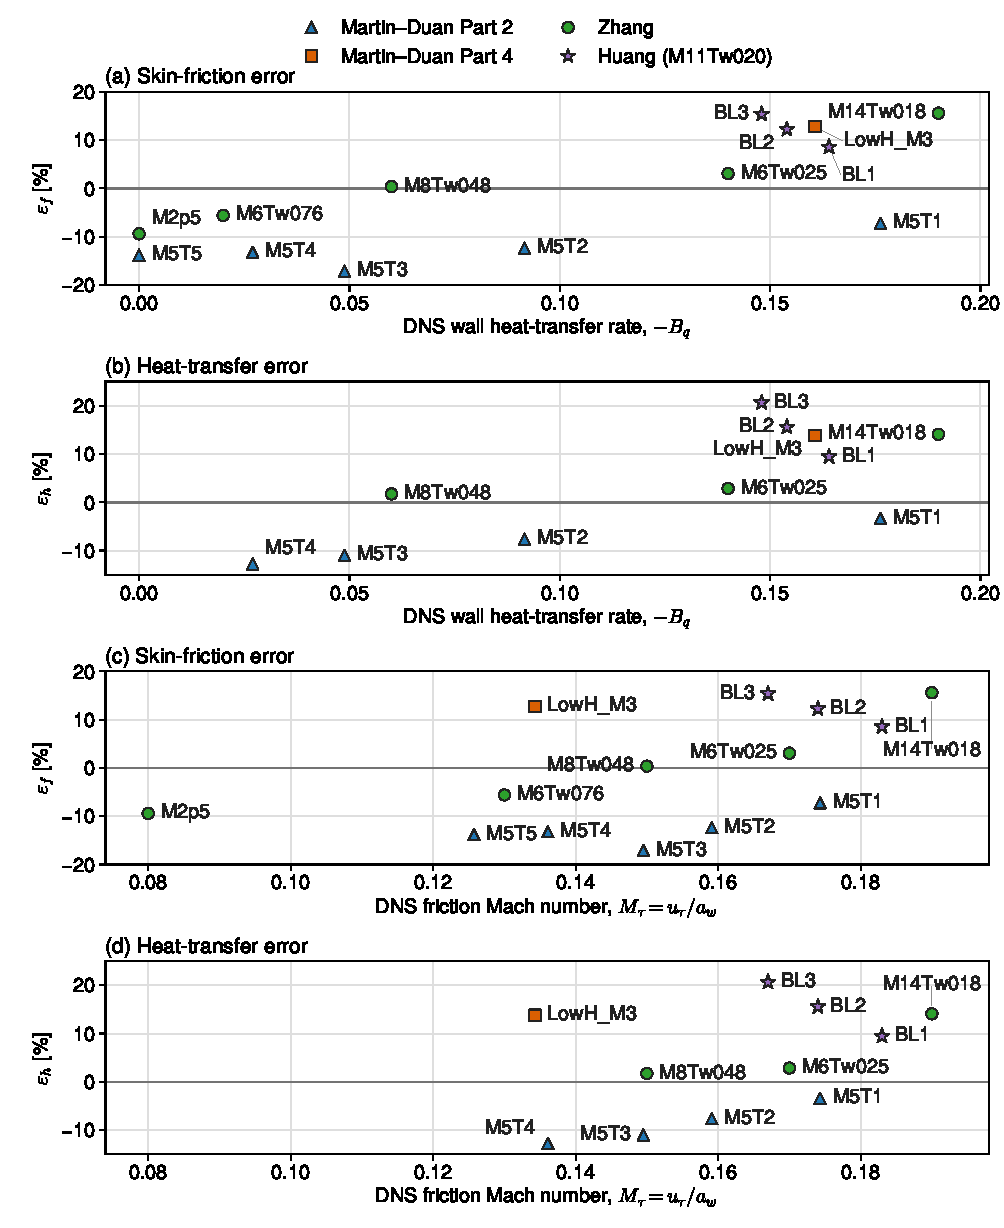
\includegraphics[width=\linewidth]{07_Error_Isolation_Results/Figures/WallResolved/DNS_Cf_Ch_relative_error_kwSST.pdf}
    \caption[Wall-resolved \(k\)--\(\omega\) SST errors in skin-friction and heat-transfer]{Signed relative errors, \(100(C_{\mathrm{RANS}}-C_{\mathrm{DNS}})/C_{\mathrm{DNS}}\), for wall-resolved \(k\)--\(\omega\) SST at \(Pr_t=0.9\). Panels (a,b): errors in the skin-friction coefficient \(C_f\) and Stanton number \(C_h\), respectively, versus the DNS dimensionless wall heat-transfer rate \(-B_q\). Panels (c,d): the corresponding errors versus the DNS friction Mach number \(M_\tau=u_\tau/a_w\). Symbols identify the DNS sources and annotations the cases; BL1--BL3 are three stations of the single Huang case. Heat-transfer errors are omitted for the adiabatic references and M6Tw076. Definitions, matching stations and reference-data limitations follow Section~\ref{sec:evaluation:benchmark-cases}.}
    \label{fig:wall-resolved:kwSST_DNS_ZPG_FPs}
\end{figure}

\begin{figure}[H]
    \centering
    % Figure provenance (WSL; absolute paths):
    %   Original retained figure: /home/mgnadlinger/ZPG_FP_overview/orig.DNS_Cf_Ch_relative_error_SA.png
    %   Updated figure: tmp/wall_resolved_table/figures/DNS_Cf_Ch_relative_error_SA.png (workspace root)
    %   Readability replot (2026-10-19): four stacked panels at the printed 170 mm
    %     width, 9.5 pt labels/ticks/legend, and vector PDF output. Exact values and
    %     omissions are retained from the audited 2026-10-14 figures above.
    %     Local regeneration: Figures/WallResolved/plot_wall_coefficient_errors.py
    %     with wall_coefficient_error_data.csv and wall_coefficient_error_provenance.json
    %     in the same directory (paths relative to this chapter).
    %   Python script:
    %     /home/mgnadlinger/ZPG_FP_overview/plot_dns_coefficient_errors.py
    %   Data / simulation roots (high-level):
    %     /home/mgnadlinger/Duan_DNS_ZPGFP/dns_comparison_SA
    %     /home/mgnadlinger/Huang_DNS_ZPGFP/dns_comparison_SA
    %     /home/mgnadlinger/Zhang_DNS_ZPGFP/dns_comparison_SA
    %     /home/mgnadlinger/Duan_DNS_ZPGFP/Martin_Duan_Part2/SA_Prt0p9
    %     /home/mgnadlinger/Duan_DNS_ZPGFP/Martin_Duan_Part4/SA_Prt0p9/LowH_M3
    %     /home/mgnadlinger/Huang_DNS_ZPGFP/SA_Prt0p9/M11Tw20
    %     /home/mgnadlinger/Zhang_DNS_ZPGFP/SA_Prt0p9
    %     /home/mgnadlinger/Duan_DNS_ZPGFP/Martin_Duan_Part2/Digitizations
    %     /home/mgnadlinger/Duan_DNS_ZPGFP/Martin_Duan_Part4/Digitizations
    %     /home/mgnadlinger/Huang_DNS_ZPGFP/References
    %     /home/mgnadlinger/Zhang_DNS_ZPGFP/References/Data
    %   Note: Updated on 2026-10-14 from the current curated comparison exports to include
    %     the corrected M5T1 Tw=228.1 K run, consistent with its appendix profile.
    %     Regeneration wrapper: tmp/wall_resolved_table/regenerate_point_only_overviews.py
    %     (workspace root); retains point-only presentation and original legend, without
    %     the trend fits added to the current external plotting script. All other values
    %     agree with the retained orig. export. Numerical audit and input snapshot are
    %     retained in tmp/wall_resolved_table/; original WSL provenance is preserved above.
    % End figure provenance.
    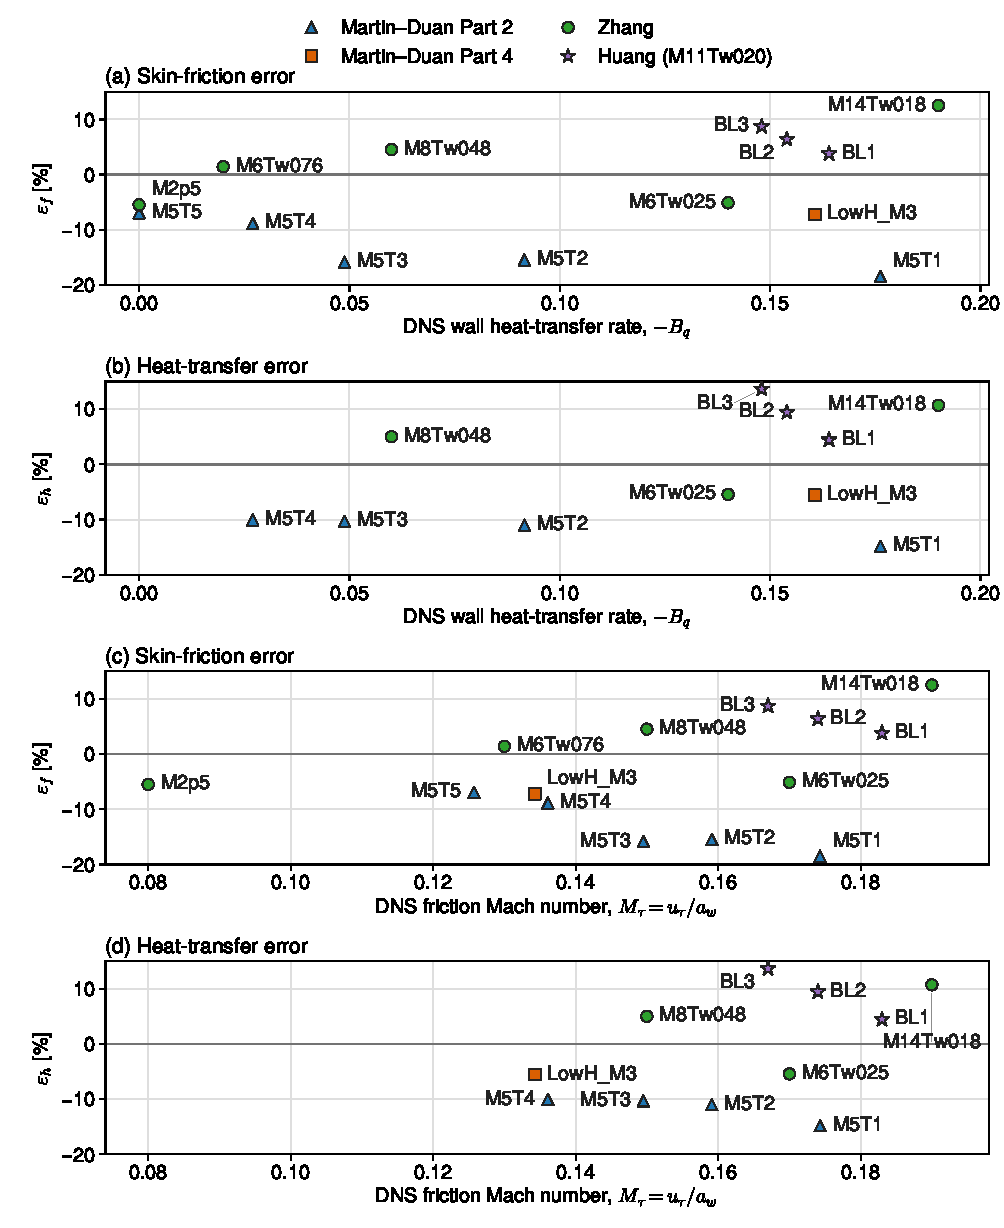
\includegraphics[width=\linewidth]{07_Error_Isolation_Results/Figures/WallResolved/DNS_Cf_Ch_relative_error_SA.pdf}
    \caption[Wall-resolved Spalart--Allmaras errors in skin-friction and heat-transfer]{Signed relative errors for the corrected wall-resolved Spalart--Allmaras model at \(Pr_t=0.9\), using the same references and definitions as Figure~\ref{fig:wall-resolved:kwSST_DNS_ZPG_FPs}. Panels (a,b): errors in \(C_f\) and \(C_h\), respectively, versus DNS \(-B_q\). Panels (c,d): the corresponding errors versus DNS \(M_\tau\). Positive values indicate overprediction of the reference coefficient. Heat-transfer errors are omitted for the adiabatic references and M6Tw076.}
    \label{fig:wall-resolved:SA_DNS_ZPG_FPs}
\end{figure}

\subsection{Boundary layer profiles and temperature--velocity relations}
\label{subsec:comparative:zpg:wr-profiles}

Wall coefficients alone do not show whether the flow supplied to a wall function has the correct internal structure. The detailed profile comparisons therefore examine both velocity and temperature, with particular emphasis on the mean temperature--velocity relation \(T(U)\) introduced in Section~\ref{subsec:background:temperature-velocity}. This relation is directly relevant to the energy closures of the investigated analytical wall functions. A discrepancy in \(T(U)\) implies that a wall closure fitted to DNS and the resolved RANS field need not describe the same relation between thermal and momentum transport, even when their wall heat-fluxes are close.
\par\medskip

Figures~\ref{fig:wall-resolved:M6Tw025_BL_Profile} and~\ref{fig:wall-resolved:LowH_M3_BL_Profile} illustrate the contrast using M6Tw025 and LowH\_M3. Corresponding comparisons for the other ten benchmark cases are provided in Appendix~\ref{app:zpg:wr-profiles}.

\begin{figure}[H]
    \centering
    % Figure provenance (WSL; absolute paths):
    %   Figure: /home/mgnadlinger/Zhang_DNS_ZPGFP/dns_comparison_SA_kwSST/figures/M6Tw025_profiles.png
    %   Python script:
    %     /home/mgnadlinger/Zhang_DNS_ZPGFP/plot_combined_dns_profiles.py
    %   Data / simulation roots (high-level):
    %     /home/mgnadlinger/Zhang_DNS_ZPGFP/SA_Prt0p9/M6Tw025
    %     /home/mgnadlinger/Zhang_DNS_ZPGFP/kwSST_Prt0p9/M6Tw025
    %     /home/mgnadlinger/Zhang_DNS_ZPGFP/References/Data
    %   Print-size replot (2026-10-19):
    %     thesis/07_Error_Isolation_Results/Figures/WallResolved/plot_wall_resolved_profiles.py
    %     Exact plotted coordinates and source hashes retained in adjacent
    %     wall_resolved_profile_data.json and wall_resolved_profile_provenance.json.
    %     Original curves/stations/panel selection preserved; 170 mm PDF, 10.5 pt text.
    % End figure provenance.
    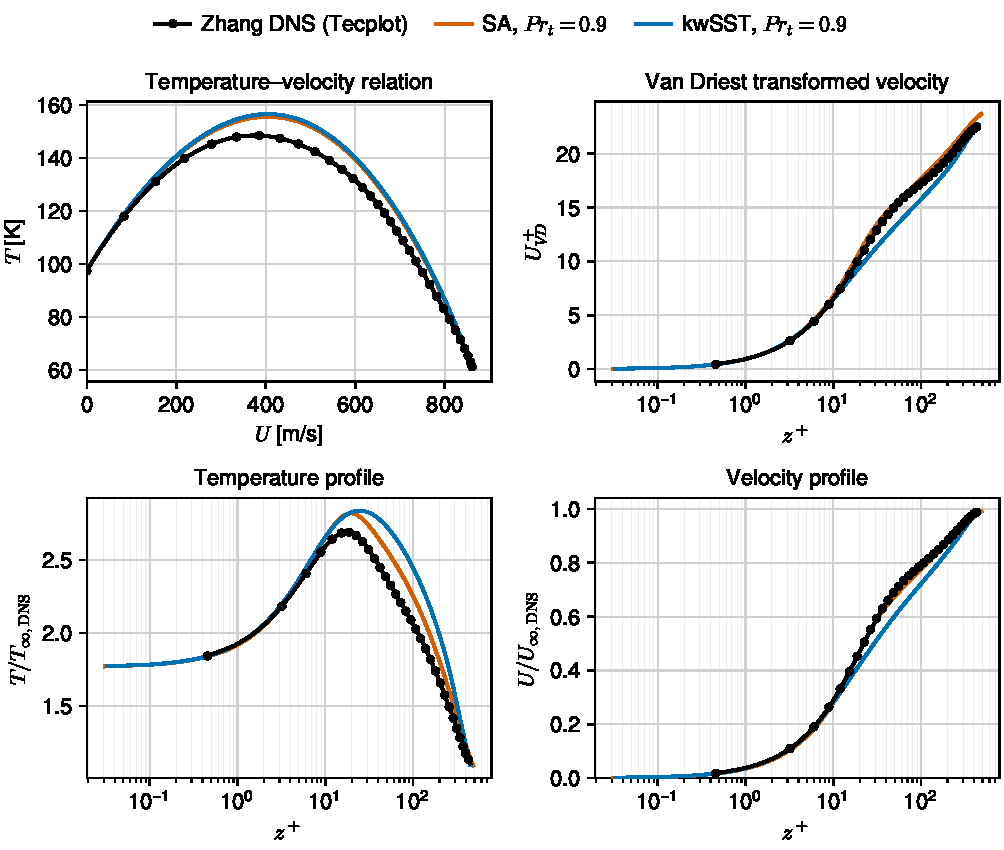
\includegraphics[width=\linewidth]{07_Error_Isolation_Results/Figures/WallResolved/M6Tw025_BL_profiles.pdf}
    \caption[M6Tw025: wall-resolved boundary layer profiles compared with DNS]{Wall-resolved Spalart--Allmaras and \(k\)--\(\omega\) SST profiles for M6Tw025 at \(Pr_t=0.9\), matched at \(Re_{\delta2}=1135\) and compared with Zhang et al.'s digital DNS profiles~\cite{zhang2018direct}. Top: dimensional temperature--velocity relation \(T(U)\) (left) and van Driest--transformed velocity \(U_{\mathrm{VD}}^+\) versus wall distance \(z^+\) (right). Bottom: normalized temperature \(T/T_{\infty,\mathrm{DNS}}\) (left) and velocity \(U/U_{\infty,\mathrm{DNS}}\) (right) versus \(z^+\). Profiles are truncated at their \(99\%\)-velocity boundary layer edge. The thermal maximum is overpredicted by both turbulence models despite differences between their velocity profiles.}
    \label{fig:wall-resolved:M6Tw025_BL_Profile}
\end{figure}

\begin{figure}[H]
    \centering
    % Figure provenance (WSL; absolute paths):
    %   Figure: /home/mgnadlinger/Duan_DNS_ZPGFP/dns_comparison_SA_kwSST/figures/Part4_LowH_M3_profiles.png
    %   Python script:
    %     /home/mgnadlinger/Duan_DNS_ZPGFP/plot_combined_dns_profiles.py
    %   Data / simulation roots (high-level):
    %     /home/mgnadlinger/Duan_DNS_ZPGFP/Martin_Duan_Part4/SA_Prt0p9/LowH_M3
    %     /home/mgnadlinger/Duan_DNS_ZPGFP/Martin_Duan_Part4/kwSST_Prt0p9/LowH_M3
    %     /home/mgnadlinger/Duan_DNS_ZPGFP/Martin_Duan_Part4/Digitizations
    %   Note: Previous thesis PNG cropped the upper two panels of the source export.
    %   Print-size replot (2026-10-19):
    %     thesis/07_Error_Isolation_Results/Figures/WallResolved/plot_wall_resolved_profiles.py
    %     Exact plotted coordinates and source hashes retained in adjacent
    %     wall_resolved_profile_data.json and wall_resolved_profile_provenance.json.
    %     Original curves/stations/panel selection preserved; 170 mm PDF, 10.5 pt text.
    % End figure provenance.
    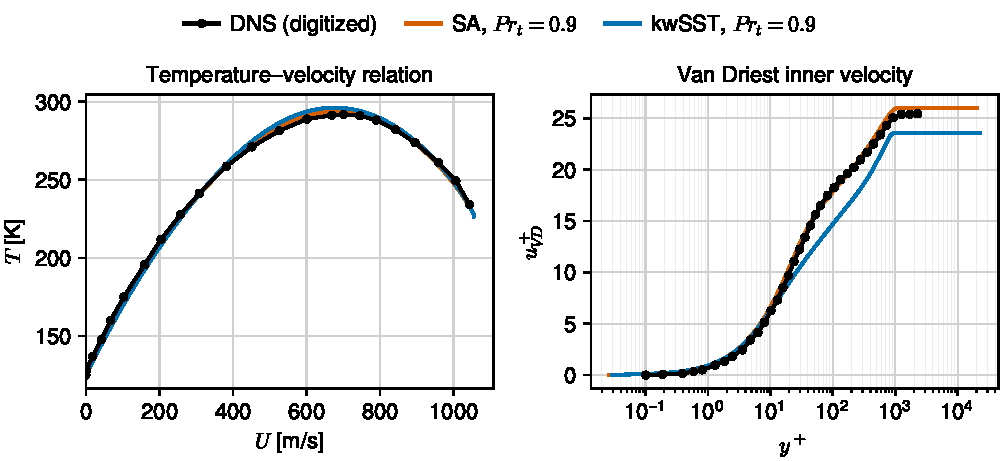
\includegraphics[width=\linewidth]{07_Error_Isolation_Results/Figures/WallResolved/Part4_LowH_M3_BL_profiles.pdf}
    \caption[LowH\_M3: wall-resolved boundary layer profiles compared with DNS]{Wall-resolved Spalart--Allmaras and \(k\)--\(\omega\) SST profiles for Martin--Duan Part~4 LowH\_M3 at \(Re_{\delta2}=1554.5\) and \(Pr_t=0.9\), compared with digitized DNS~\cite{duan2011direct_Part4}. Left: dimensional temperature--velocity relation \(T(U)\). Right: van Driest--transformed velocity \(U_{\mathrm{VD}}^+\) versus wall distance \(y^+\). The DNS wall-normal reconstruction retains the provisional boundary layer-edge endpoint assumption indicated in the plot. Both models closely reproduce the displayed \(T(U)\) relation, while their transformed velocity profiles differ.}
    \label{fig:wall-resolved:LowH_M3_BL_Profile}
\end{figure}

For M6Tw025, both Spalart--Allmaras and \(k\)--\(\omega\) SST overpredict the temperature maximum and the recovering part of the thermal profile (see Figure~\ref{fig:wall-resolved:M6Tw025_BL_Profile}). Their \(T(U)\) curves are very similar, although the transformed velocity profiles and the locations of the thermal maximum in wall units differ. SST's close wall-coefficient agreement (see Figure~\ref{fig:wall-resolved:kwSST_DNS_ZPG_FPs}) consequently coexists with a visibly incorrect thermal profile. SA, meanwhile, follows the displayed velocity profiles comparatively closely despite its thermal discrepancy. Section~\ref{subsec:erriso:rans-profile-influence} tests the consequence for wall-function heating by applying the same Li closure to the DNS and resolved SA profiles.
\par\medskip

The LowH\_M3 case presents the complementary behaviour: both models closely reproduce the displayed \(T(U)\) relation (see Figure~\ref{fig:wall-resolved:LowH_M3_BL_Profile}), yet their wall coefficients retain appreciable errors, especially for SST (see Figure~\ref{fig:wall-resolved:kwSST_DNS_ZPG_FPs} and Figure~\ref{fig:wall-resolved:SA_DNS_ZPG_FPs}). Among the selected cold-wall cases, LowH\_M3 provides the only qualitatively close agreement in the thermal \(T(U)\) relation.
\par\medskip

This distinction follows from the derivative character of the wall quantities. As described in Section~\ref{sec:openFOAM_qw_tauw}, resolved wall heat-flux and shear stress depend on the temperature and velocity gradients at the wall. A profile can agree over much of the boundary layer while retaining a different wall gradient and conversely, a similar wall gradient does not establish agreement throughout the profile. Visual comparison of \(T(U)\) therefore complements the coefficient errors and cannot replace them. The same reasoning will apply to the wall-function closures: a visually close temperature--velocity relation is insufficient to establish the accuracy of the wall quantities recovered from it.

\subsection{Evidence concerning the turbulent Prandtl number}
\label{subsec:comparative:zpg:wr-prandtl}

The similarity of the SA and SST \(T(U)\) discrepancies throughout all but one of the investigated hypersonic cold-wall ZPG FP cases motivates examination of their common thermal closure. Both extend the eddy viscosity to thermal transport through \(\kappa_t=c_p\mu_t/Pr_t\). Fixing \(Pr_t\) fixes the local ratio of modelled turbulent momentum and thermal diffusivity, even though their physical relationship may vary across a cold-wall boundary layer.
\par\medskip

Figure~\ref{fig:evaluation:turb_prandtl_comparison} compares the DNS turbulent-Prandtl-number distributions across the boundary layer with the adopted constant value of \(Pr_t = 0.9\). It is clearly visible, that much of the outer boundary layer has values of order unity - arguing for a constant \(Pr_t\) - but the near-wall regions show pronounced variation, overshoots and sign changes. This also uncovers a notable difference in the LowH\_M3 and M6Tw025 case, which may explain their difference in the ability of the turbulence model to reprduce their thermal boundary layer profile (see Figure~\ref{fig:wall-resolved:LowH_M3_BL_Profile} vs. ~\ref{fig:wall-resolved:kwSST_DNS_ZPG_FPs}). The LowH\_M3 case recovers toward values near unity after its sharp near-wall excursion, whereas the M6Tw025 distribution falls below unity over a broader part of the inner boundary layer. So while the constant \(Pr_t = 0.9\) is still a reasonable assumption for for hypersonic adiabatic wall cases and in the outer region of hypersonic cold-wall cases, it is not in the near-wall region for the majority of the hypersonic cold-wall cases. From this analysis, it is not possible to conclude that the turbulent Prandtl number is the sole cause of the observed discrepancies, but it is a plausible contributor. As discussed in later Section~\ref{subsec:comparative:zpg:case-selection} this work can also not find an immediate explanation for the difference in the turbulent Prandtl number distributions between the two cases.
\par\medskip

The sharply varying DNS values require particular care. The diagnostic \(Pr_t\) is obtained from turbulent fluxes and mean gradients, rather than being an independently measured transport constant. Duan and Martin associate its overshoots and sign changes with the crossover locations of the turbulent heat-flux and mean temperature gradient~\cite[Section~5]{duan2011direct_Part4}. Near these locations the inferred local ratio can become poorly conditioned, and a temperature maximum alone does not imply a divergence of \(Pr_t\). Such behaviour also exposes limitations of describing the turbulent thermal flux everywhere by a positive scalar diffusivity and a local temperature gradient. Directly substituting the displayed singular or negative values into the present RANS closure would therefore require a different modelling argument.

\begin{figure}[H]
    \centering
    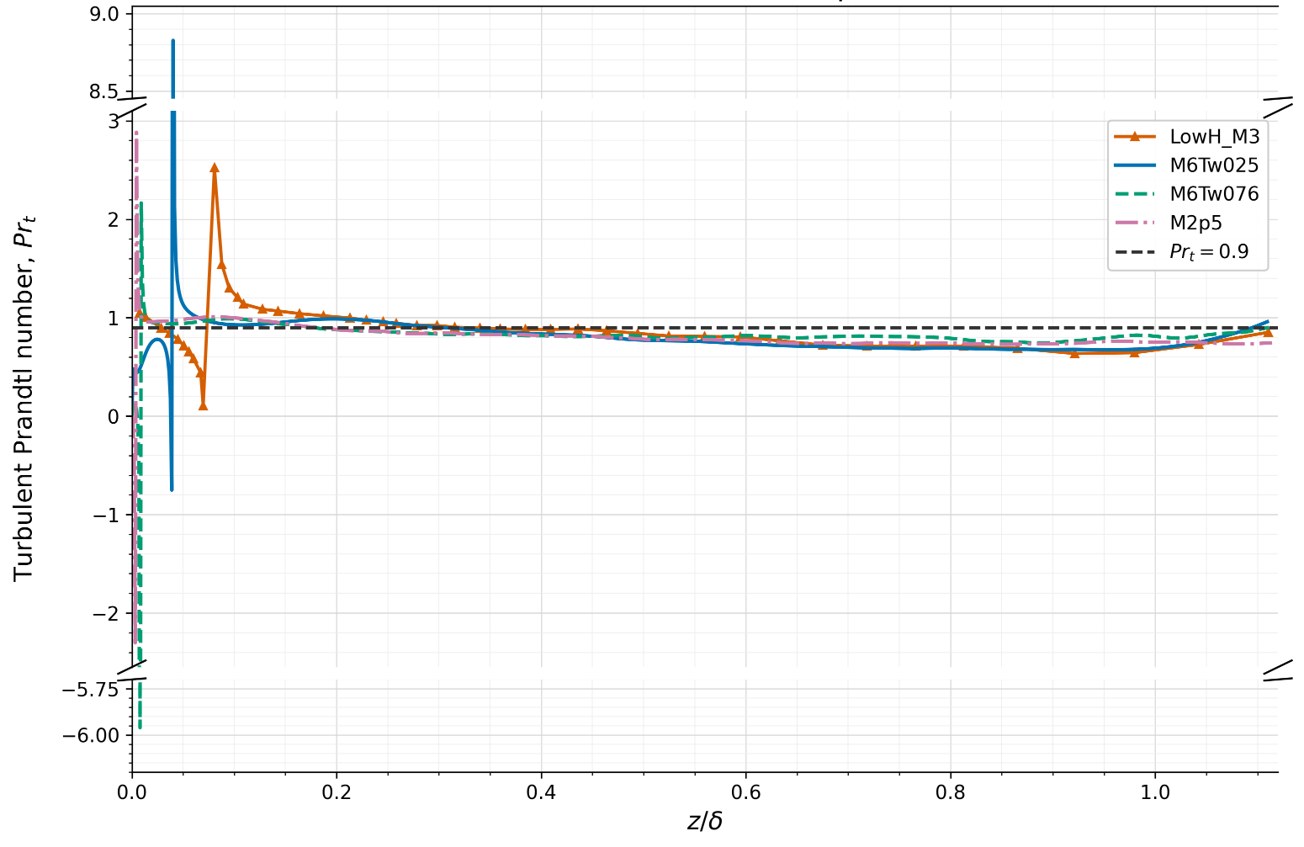
\includegraphics[width=0.8\linewidth]{06_Eval_Methodology/06_Figures/Turb_Prandtl_Number_Comparison.png}
    \caption[DNS turbulent-Prandtl-number distributions]{Turbulent Prandtl number across the whole boundary layer height, with wall-normal distance \(z\) normalized by the respective boundary layer thickness \(\delta\). M2p5, M6Tw025 and M6Tw076 use Zhang et al.'s DNS data~\cite{zhang2018direct}; LowH\_M3 uses the digitized Martin--Duan Part~4 distribution~\cite{duan2011direct_Part4}. The dashed horizontal line marks the RANS value \(Pr_t=0.9\). Breaks in the vertical axis retain the large excursions near the wall while exposing the order-unity variation over the rest of the profile. The M2p5 and M6Tw076 are adiabatic cases, whereas LowH\_M3 and M6Tw025 are strongly cold-wall cases (see Section~\ref{sec:evaluation:benchmark-cases}).}
    \label{fig:evaluation:turb_prandtl_comparison}
\end{figure}

The RANS \(Pr_t\)sensitivity calculations represented in Figure~\ref{fig:evaluation:turb_prandtl_comparison_thermal_profile} provides further evidence that the thermal closure materially affects the \(T(U)\) profile. Reducing the constant \(Pr_t\) from \(1.0\) to \(0.6\) lowers the predicted temperature maximum in both models and brings it closer to DNS. No displayed constant reproduces the entire relation: the curves retain differences on the upper,  recovering region. This aligns with the previous observation that the M6Tw025 case has a near-wall \(Pr_t\) distribution that remains below unity over a broader part of the inner boundary layer.

\begin{figure}[H]
    \centering
    % Figure provenance and typography restoration (2026-10-19):
    %   Original high-resolution export: ../Weekly 260803.pptx, slide 21,
    %     archive member ppt/media/image13.png (3189 x 1232 pixels).
    %   Retained source and reproduction script:
    %     thesis/06_Eval_Methodology/06_Figures/thermal_BL_profile_Prt_source/
    %     original_export.png, restore_typography.py and provenance.json.
    %   Original sensitivity-study data/script were not located. Curve pixels
    %     are preserved; axes/ticks/legends are replaced with larger vector text.
    %     This restores typography rather than replotting numerical data.
    % End figure provenance.
    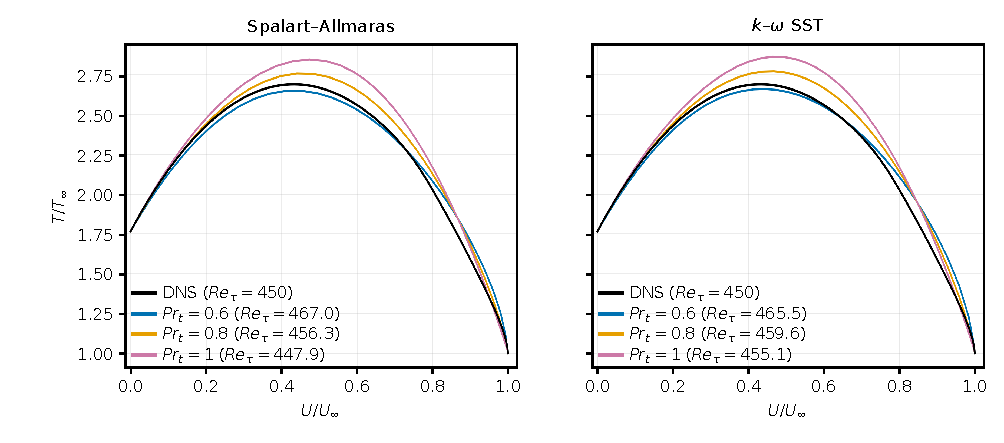
\includegraphics[width=\linewidth]{06_Eval_Methodology/06_Figures/thermal_BL_profile_Prt.pdf}
    \caption[Effect of constant \(Pr_t\) on the M6Tw025 temperature--velocity relation]{Sensitivity of the M6Tw025 mean temperature--velocity relation to constant \(Pr_t=0.6\), \(0.8\) and \(1.0\) in wall-resolved SA (left) and \(k\)--\(\omega\) SST (right). Temperature and velocity are normalized by the freestream values. The DNS reference has \(Re_\tau=450\); the RANS stations have approximately \(448\leq Re_\tau\leq467\), as listed in the legends. These stations differ from the \(Re_{\delta2}\)-matched baseline protocol. Lower \(Pr_t\) reduces the thermal maximum but does not remove the discrepancy over the complete relation.}
    \label{fig:evaluation:turb_prandtl_comparison_thermal_profile}
\end{figure}

Taken together, the DNS distributions, the similar thermal-profile errors of two different momentum closures, and the constant-\(Pr_t\) sensitivity identify the thermal closure as a plausible contributor to the discrepancies. They do not isolate it from errors in the eddy viscosity or from other modelling assumptions. Related hypersonic calculations by Huang et al. found improved temperature predictions with an algebraic turbulent-energy-flux closure compared with constant \(Pr_t\), using an algebraic momentum model~\cite{huang2020simulation}. That result supports further investigation of the thermal closure, while its different momentum model prevents direct attribution of the present SA and SST errors to \(Pr_t\) alone.
\par\medskip

\subsection{Assessment of results and comparison to existing publications}
\label{subsec:comparative:zpg:results-assessment}

Several published RANS assessments use the Zhang and Huang benchmarks included in Table~\ref{tab:evaluation:selected-cases}. They provide context for the wall-load errors and thermal-profile discrepancies found here, but common case and model names do not ensure equivalent calculations. The following comparison identifies differences in model formulation, mean-flow coupling, inflow conditions and sampling location that affect interpretation of Table~\ref{tab:wall-resolved:coefficients}.

\paragraph*{Huang et al. (2019)}

Huang et al.~\cite{huang2019assessment} assess SA and SST for M8Tw048 and report wall-coefficient errors within \(5\%\), broadly consistent with the small errors obtained here for this case. Their calculations use \(Pr_t=0.85\) and \(Re_\tau\) matching, whereas the present baseline uses \(Pr_t=0.9\) and \(Re_{\delta2}\) matching (Section~\ref{subsec:evaluation:matching-station}). Moreover, reconstructing the DNS heat-flux from the published, rounded \(-B_q\) introduces a \(\pm8.33\%\) rounding bound (Table~\ref{tab:evaluation:zhang-bq-rounding}). This limits comparisons based on that reconstruction and it is not an uncertainty estimate for Huang et al.'s underlying DNS data.

\paragraph*{Aiken et al. (2022)}

Aiken et al.~\cite{aiken2022assessment} assess SA, \(k\)--\(\omega\) BSL and SST against six Zhang and Huang benchmarks at \(Pr_t=0.9\). They report thermal-profile discrepancies similar to those in Section~\ref{subsec:comparative:zpg:wr-profiles} and identify the thermal closure as a possible contributor. Their tested freestream-turbulence variations have little downstream influence for M8Tw048. However, their SA model includes the Catris--Aupoix correction, distinct from the implementation correction in Section~\ref{subsec:ext:spalart-allmaras-of-correction}, and their original SST formulation differs from the updated version described in Section~\ref{sec:background:rans-turbulence-modelling}. They match \(Re_\tau\), while reporting similar errors with \(Re_\theta\) matching. Their Table~1 also lists total enthalpies inconsistent with the stated flow conditions, and Table~3 contains inconsistent \(Re_\theta/\theta\) values for M8Tw048. These reporting issues limit reproducibility without establishing that the imposed flow states were incorrect. Together with the formulation differences, they prevent treating agreement or disagreement as a direct code-verification result, consistent with the reporting concerns of Viti et al.~\cite{viti2007numerical}.

\paragraph*{Danis (2023)}

Danis~\cite[Figure~4.10]{danis2023direct} compares original SST skin-friction predictions with DNS for M6Tw025, M14Tw018 and M11Tw020 as functions of \(Re_\tau\), without a corresponding SST wall-heat-flux comparison. The calculations use VULCAN-CFD and cite Menter's 1994 SST model, but the turbulent Prandtl number and detailed model settings are not specified in that assessment. Differences from the present skin-friction results therefore cannot be attributed to a particular modelling or implementation choice.

\paragraph*{Vaughan et al. (2025)}

Vaughan et al.~\cite{vaughan2025paper} and Vaughan's master's thesis~\cite{vaughan2025thesis} examine overlapping Zhang and Huang cases. The thesis likewise finds cold-wall thermal-profile discrepancies at \(Pr_t=0.9\), but uses SA-neg and a vorticity-based SST limiter, rather than the present model variants. It selects sampling locations by matching the initial DNS boundary layer thickness and then advancing by the reported downstream distance, rather than matching \(Re_\tau\). This is the shifted-station approach discussed in Section~\ref{subsec:evaluation:matching-station}.
\par\medskip

For SST, Vaughan's documented mean-flow equations retain the isotropic turbulent stress, turbulent kinetic energy in total energy, and its diffusive transport, whereas the present HiSA formulation omits these contributions. Zhang et al.~\cite{zhang2021formulation} found sensitivity to these terms in shock interactions but little influence on skin-friction and velocity profiles for their single Mach-5 flat-plate. That result does not establish negligible heating sensitivity for the present cases.
\par\medskip

Vaughan also interprets the DNS freestream states as post-shock values and supplies modified pre-shock inflows~\cite[Tables~2.2--2.3]{vaughan2025thesis}. The reconstruction procedure is unspecified and a discrepancy arises for M14Tw018, where the tabulated pre-shock mean-flow total enthalpy \(c_pT+U^2/2\) exceeds the DNS value by \(4.56\%\). Table~\ref{tab:inflow-comparison} tests these inflows in the present SST implementation for four Zhang cases, retaining each run's own \(Re_{\delta2}\)-matched station. This demonstrates sensitivity to the inflow specification, but neither establishes which inflow better reproduces DNS nor reproduces Vaughan's complete setup.

% Data: /home/mgnadlinger/Zhang_DNS_ZPGFP/kwSST_Prt0p9/inflow_comparison_20261017/comparison_native_with_DNS.csv
% Extraction: add_dns_reference.py --matching native in the same directory;
% station and DNS-reference provenance: DNS_reference_native_audit.json.
\begin{table}[H]
    \centering
    \caption[Inflow sensitivity of wall-resolved SST wall loads]{Inflow sensitivity of the present wall-resolved \(k\)--\(\omega\) SST simulations against Zhang's DNS~\cite{zhang2018direct}. Original inflows use the DNS freestream conditions in Table~\ref{tab:evaluation:zhang-inflow-wall}; modified inflows use Vaughan's pre-shock values~\cite[Table~2.2]{vaughan2025thesis}. Each run is evaluated at its own \(Re_{\delta2}\)-matched station using its respective inlet density and velocity. Parentheses give \(100(\mathrm{RANS}-\mathrm{DNS})/\mathrm{DNS}\). Heat-flux is positive into the wall; shear stress is its magnitude. The M6Tw076 heat-flux reference is nominal and retained only for this sensitivity comparison, subject to the rounding and wall-temperature limitations in Section~\ref{sec:evaluation:benchmark-cases}.}
    \label{tab:inflow-comparison}
    \small
    \begin{tabular}{@{}llrr@{}}
        \toprule
        Case & Reference / inflow & \(q_w\) [\(\mathrm{kW\,m^{-2}}\)] & \(\tau_w\) [\(\mathrm{Pa}\)] \\
        \midrule
        M6Tw025 & \textbf{Zhang DNS} & \textbf{11.4888} & \textbf{28.3210} \\
        M6Tw025 & Original & 11.8290 (\(+2.96\%\)) & 29.2326 (\(+3.22\%\)) \\
        M6Tw025 & Vaughan & 11.4180 (\(-0.62\%\)) & 28.2175 (\(-0.37\%\)) \\
        \addlinespace
        M6Tw076 & \textbf{Zhang DNS} & \textbf{2.1720} & \textbf{16.2533} \\
        M6Tw076 & Original & 1.8925 (\(-12.87\%\)) & 15.3712 (\(-5.43\%\)) \\
        M6Tw076 & Vaughan & 1.8585 (\(-14.43\%\)) & 15.1801 (\(-6.60\%\)) \\
        \addlinespace
        M8Tw048 & \textbf{Zhang DNS} & \textbf{4.5495} & \textbf{13.2915} \\
        M8Tw048 & Original & 4.6231 (\(+1.62\%\)) & 13.3289 (\(+0.28\%\)) \\
        M8Tw048 & Vaughan & 4.5881 (\(+0.85\%\)) & 13.2067 (\(-0.64\%\)) \\
        \addlinespace
        M14Tw018 & \textbf{Zhang DNS} & \textbf{10.3028} & \textbf{12.1640} \\
        M14Tw018 & Original & 11.7582 (\(+14.13\%\)) & 14.0633 (\(+15.61\%\)) \\
        M14Tw018 & Vaughan\textsuperscript{*} & 12.3612 (\(+19.98\%\)) & 14.3311 (\(+17.82\%\)) \\
        \bottomrule
    \end{tabular}
    \par\smallskip
    \begin{minipage}{\linewidth}
        \footnotesize
        \textsuperscript{*} Vaughan's tabulated M14Tw018 pre-shock mean-flow total enthalpy \(c_pT+U^2/2\) is \(4.56\%\) higher than that of the DNS freestream state.
    \end{minipage}
\end{table}

\paragraph*{Cheng et al. (2026)}

Cheng et al.~\cite{cheng2026reynolds} use OpenFOAM-v2312 and the HiSA solver framework to investigate energy closures with the Durbin--Yin \(k\)--\(\omega_0\) model, including additional SST--\(\omega_0\) tests. Their baseline therefore differs from the present SST model even before the proposed energy-closure corrections. Their stated energy equation includes turbulent-kinetic-energy transport~\cite[Eq.~2.7]{cheng2026reynolds}, which is absent from the present HiSA formulation. The paper does not specifically state having performed the corresponding solver modifications outside of the stated RANS equations. Shared solver ancestry consequently does not establish equivalent mean-flow coupling. Station selection adds another difference, although the present tests in Tables~\ref{tab:evaluation:matching-station-bq} and~\ref{tab:evaluation:matching-station-ch} give changes below \(1\%\) in \(-B_q\) and \(2\%\) in \(C_h\) between the shifted and \(Re_{\delta2}\)-matched stations. Their Table~5 also normalizes \(B_q\) with DNS wall quantities, whereas Table~\ref{tab:wall-resolved:coefficients} uses each solution's own wall state. These values require consistent normalization before comparison.

\paragraph*{Implications for the present assessment}

The literature supports treating the present discrepancies as part of a broader difficulty in predicting cold-wall boundary layers with conventional RANS closures. It does not provide an equivalent setup for direct code verification or isolate the cause of differences in wall loads. In particular, the thermal-profile deficiencies reported by Aiken and Vaughan reinforce the evidence in Sections~\ref{subsec:comparative:zpg:wr-profiles} and~\ref{subsec:comparative:zpg:wr-prandtl}, without establishing constant \(Pr_t\) as their sole cause. The subsequent wall-function assessment therefore retains both DNS and the present wall-resolved SA solution as distinct references, as defined in Table~\ref{tab:erriso:reference-hierarchy}.

\subsection{Selection of cases for detailed wall-function assessment}
\label{subsec:comparative:zpg:case-selection}

M6Tw025 and LowH\_M3 are retained for the detailed coupled wall-function analysis because they expose different relationships between wall-coefficient and profile accuracy. M6Tw025 supplies digital DNS profiles for a strongly cooled Mach-6 boundary layer and exhibits a clear thermal-profile discrepancy in both RANS models. It therefore tests the wall functions when their analytical thermal relation is coupled to a resolved RANS field that already differs from DNS. Its detailed reference profiles also permit an independent prescribed-profile closure assessment, subject to the heat-flux reporting limitations stated above.
\par\medskip

LowH\_M3 supplies a cold-wall supersonic comparison in which the resolved RANS \(T(U)\) relation closely follows the digitized DNS. This reduces the pronounced thermal-profile mismatch present in M6Tw025 and makes the case useful for examining additional errors introduced by the wall function and the CFD mesh. The nonzero wall-coefficient errors remain part of its baseline. In the subsequent prescribed-profile calculations, the resolved SA field is used as the LowH\_M3 input, so those closure errors measure consistency with SA rather than an independent reconstruction of DNS wall quantities.
\par\medskip

The contrasting thermal-profile accuracy of LowH\_M3 and M6Tw025 cannot be attributed to the models' incompressible origins alone. The corresponding DNS studies~\cite{zhang2018direct,duan2011direct_Part4} report approximate Morkovin-type similarity and outer-layer agreement with modified strong Reynolds analogies for both cases (ref. Section \ref{subsec:background:SRA-Morkovin}). This weakens an explanation based on a fundamental loss of applicability between the two flow conditions, without excluding differences in intrinsic compressibility, mean-property gradients or thermal transport. The cause of the contrast remains unresolved, with the following analysis therefore examining the shared constant turbulent Prandtl number as a possible contributor.

\section{Wall-function closure assessment}
\label{sec:comparative:zpg:cross-comparison}

The previous wall-resolved assessment established the discrepancy of the underlying RANS calculation from DNS. Adding a wall function to a RANS simulation introduces a further relationship between the sampled flow state and the resulting wall shear stress and heat-flux. To examine that relationship separately, the analytical closures are now evaluated on prescribed boundary layer profiles. This a-priori assessment asks how well a closure can recover the known wall heat-flux and shear stress, when its off-wall sampled inputs are ideal, i.e. supplied from the respectilve known reference boundary layer profile. It provides the comparison needed to distinguish a wall function's underlying closure behaviour from the additional changes that occur when the same wall function is coupled to full FVM CFD simulation.
\par\medskip

The detailed discussion focuses on M6Tw025 and LowH\_M3, which also carry the comparison into the subsequent coupled CFD assessment (as established in Section~\ref{subsec:comparative:zpg:case-selection}). The initial M6Tw025 sweeps use the digitally published DNS profiles and wall quantities of Zhang et al.~\cite{zhang2018direct}. LowH\_M3 lacks similar high quality published DNS reference data, so it uses the wall-resolved SA profile and its corresponding wall quantities at the matched comparison station (Section~\ref{subsec:evaluation:matching-station}) are used. For LowH\_M3, the reported closure errors are thus relative to the wall-resolved SA wall quantities. An additional M6Tw025 comparison in Section~\ref{subsec:erriso:rans-profile-influence} applies the same Li closure to DNS and resolved SA inputs to assess the influence of the supplied profile. Results for the additional cases are collected in Appendix~\ref{app:zpg:apriori}.

\subsection{A-priori inverse solution}
\label{subsec:erriso:apriori-solver}

For an a-priori assessment, a virtual sampling point is moved through a known, resolved boundary layer profile. At every sampling height, the required velocity and thermodynamic state are interpolated from that given profile and supplied to the wall-function closure equations, together with the required physical wall temperature and transport properties. The wall heat-flux and shear stress are then recovered by an inverse solution of the closure equations. The reference friction velocity defines the sampling coordinate,
\begin{equation}
    y_{\mathrm{ref}}^+
    = \frac{\rho_{w,\mathrm{ref}}u_{\tau,\mathrm{ref}}y}
    {\mu_{w,\mathrm{ref}}},
    \qquad
    u_{\tau,\mathrm{ref}}
    = \sqrt{\frac{\tau_{w,\mathrm{ref}}}{\rho_{w,\mathrm{ref}}}}.
\end{equation}

For the Li formulation, introduced in Section~\ref{subsec:wall-functions:gao-li:governing-relations}, the first-point velocity and enthalpy, the physical wall state, and an arbitrarily placed second reference state determine the generalized enthalpy--velocity relation. Two reference choices are examined. The two-point construction assumes two virtual cells of equal height, so their centres satisfy \(y_2=3y_1\). Both point states are interpolated from the resolved profile. In the alternative construction, the reference state is prescribed at the boundary layer edge. Li et al propses the former, two-point construction, so that the wall function closures are independant of the boundary layer edge quantities \cite{li2025WF}, for comparison and evaluation the latter, boundary layer edge construction was selected to be included in the analysis. In either case, the unified velocity law is inverted for \(u_\tau\), and the wall outputs follow from \(\tau_w=\rho_wu_\tau^2\) and the wall function's heat-flux relation.
\par\medskip

For the Griffin formulation, introduced in Section~\ref{subsec:wall-functions:griffin:governing-relations}, the sampled velocity and thermodynamic state are combined with the wall temperature and boundary layer-edge quantities - Griffin et al do not propose a specific approach to allow for a two-point, boundary layer edge free construction. For each sample point, the inverse-transformation model is integrated from the wall region to the sample point. The wall stress is iterated until the integrated velocity reproduces the prescribed matching point's velocity. The temperature--velocity relation then supplies the wall heat-flux. The prescribed wall stress and heat-flux of the reference profile are used to assess the recovered outputs, rather than imposed as their solution targets.
\par\medskip

Edge states are supplied according to the available reference data. Griffin uses the supplied \(\delta_{99}\) for the Zhang DNS profiles and its edge criterion for LowH\_M3, whereas the prescribed-edge Li comparison for LowH\_M3 uses the \(U=0.99U_\infty\) crossing.
\par\medskip

The reported errors in this section are signed relative differences,
\begin{equation}
    \varepsilon_X
    = 100\left(\frac{X_{\mathrm{closure}}}{X_{\mathrm{ref}}}-1\right),
    \qquad X\in\{\tau_w,q_w\}.
    \label{eq:erriso:apriori-relative-error}
\end{equation}

The reference being either the DNS wall quantities or the wall-resolved RANS quantities, depending on the profile being sampled. The a-priori assessment is therefore a standalone evaluation of the closure's ability to recover the known wall fluxes from known inputs, and thus evaluates the wall function's closure theories in isolation.

\paragraph*{Consistency with the published Griffin assessment}
An independent check of the herin implemented a-priori solver on the Griffin evaluation is available from the a-priori results of Griffin et al.~\cite[Figure~5]{griffin2023WF}. Their matching height is \(y_m=0.3\delta_{99}\). In reference wall units, this corresponds to \(y_m^+=0.3\mathrm{Re}_\tau\). Table~\ref{tab:erriso:Griffin-a-priori-validation} compares the present inverse solutions at those heights with the errors read from the published figure for two identifiable Zhang cases.

\begin{table}[H]
    \centering
    \caption[Consistency check of the Griffin a-priori solver]{Comparison of the present Griffin a-priori solver at \(y_m=0.3\delta_{99}\) with Griffin et al.~\cite[Figure~5]{griffin2023WF}. Published errors are approximate values read from the figure; the comparison checks consistency of the standalone closure evaluation.}
    \label{tab:erriso:Griffin-a-priori-validation}
    \begin{tabular}{@{}l
        S[table-format=3.3]
        S[table-format=\approx-2]
        S[table-format=-2.2]
        S[table-format=\approx-2]
        S[table-format=-2.2]@{}}
        \toprule
        & & \multicolumn{2}{c}{\(\tau_w\) error [\%]} & \multicolumn{2}{c}{\(q_w\) error [\%]} \\
        \cmidrule(lr){3-4}\cmidrule(l){5-6}
        Case & {\(y_m^+\)} & {Griffin et al.} & {Present solver} & {Griffin et al.} & {Present solver} \\
        \midrule
        M6Tw025  & 134.561 & \approx -13 & -11.56 & \approx -15 & -15.28 \\
        M14Tw018 & 192.588 & \approx -10 & -11.32 & \approx -15 & -15.91 \\
        \bottomrule
    \end{tabular}
\end{table}

The present solutions reproduce the sign and approximate magnitude of the published errors to within the uncertainties of the published graph's resolution. Their agreement supports the use of the a-priori solver used in the following to examine matching-height sensitivity of the closure theories.

\subsection{Closure errors versus sampling height}
\label{subsec:erriso:apriori-results}

Figures~\ref{fig:wall-closure:a-priori-Li-M6Tw025}--\ref{fig:wall-closure:a-priori-Griffin-LowHM3} assess the closures by Li and Griffin jointly on the M6Tw025 DNS profile and the LowH\_M3 wall-resolved SA profile. Both formulations recover the wall quantities with significant errors over the varying sampling height, but neither is notably more accurate than the other. But it shows, that the Li's two-reference-point method, rather than relying on boundary layer edge quantities, works without a systematic loss of accuracy (e.g. see Figure~\ref{fig:wall-closure:a-priori-Li-M6Tw025} dashed vs. solid line). And it should be note that both Li and Griffin's formulations don't show significantly higher errors in the buffer layer, highlighting that the blending between the sublayer and law-of-the-wall for these adaptive wall functions work well and doesn't present a \(y^+\) meshing region to be specifically avoided.
\par\medskip

Across all the investigated profiles (including the cases in Appendix~\ref{app:zpg:apriori}) Griffin gives signed shear-stress errors of approximately \(-11\%\) to \(+11\%\) and heat-flux errors of \(-14\%\) to \(+6\%\), over the reasonable range of \(1\le y_{\mathrm{ref}}^+\le100\). Over the same cases and sampling-height interval, the Li closure gives respective shear-stress errors of approximately \(-7\%\) to \(+13\%\) and heat-flux errors of \(-15\%\) to \(+18\%\). These are appreciable closure errors for prescribed, ideal, inputs and warrant ongoing research into finding better velocity transformation like by Hasan et al.\cite{hasan2023incorporating} and improved closure formulations.
\par\medskip

The heat-flux ranges exclude M2p5, whose adiabatic reference makes relative heat-flux errors undefined, and M6Tw076, owing to the reference-data limitations described in Section~\ref{sec:evaluation:benchmark-cases}.
\par\medskip

At the largest sampling height, Li's prescribed-edge M6Tw025 heat-flux error rises to approximately \(+79\%\) at \(y_1^+=400\), with a reported \(Re_\tau = 450\) \cite{zhang2018direct}, this corresponds to a sampling station at about \(0.89\delta_{99}\). Li's two-reference point method, is not applicable anymore at these sampling stations because the second reference point sits outside of the boundary layer, this is a limit of this method. The high error at these high sampling points, is consistent with increasing sensitivity of the enthalpy inversion as the sampled and reference velocities approach one another, especially because the first sampling point also lies outside the inner layer~\cite[Eq.~(40)]{li2025WF}. Griffin avoids this particular inversion sensitivity by prescribing the wall temperature--velocity slope through its Reynolds analogy. It shows significant improvement to this high \(y^+\) sensitivity, but does not establish universal validity near the boundary layer edge. The published a-priori comparison uses \(y_m=0.3\delta_{99}\); the additional WMLES matching-height studies discussed in Section~\ref{subsec:wall-functions:griffin:validation-scope} do not extend this assessment towards the edge.

\clearpage

\begin{figure}[H]
    \centering
    % Figure provenance (WSL; absolute paths):
    %   Figure: /home/mgnadlinger/OpenFOAM/mgnadlinger-v2412/src/LiWallFunctions/tests/ReverseSolver/M6Tw025_Stat_Zhang/wall_flux_errors_vs_yplus.png
    %   Python scripts:
    %     /home/mgnadlinger/OpenFOAM/mgnadlinger-v2412/src/LiWallFunctions/tests/ReverseSolver/plot_m6tw025_flux_reference_overlay.py
    %     /home/mgnadlinger/OpenFOAM/mgnadlinger-v2412/src/LiWallFunctions/tests/ReverseSolver/analyze_li_wall_function_profile_Zhang.py
    %   Data / simulation roots (high-level):
    %     /home/mgnadlinger/OpenFOAM/mgnadlinger-v2412/src/LiWallFunctions/tests/ReverseSolver/M6Tw025_Stat_Zhang
    %     /home/mgnadlinger/OpenFOAM/mgnadlinger-v2412/src/LiWallFunctions/tests/ReverseSolver/M6Tw025_Stat_Zhang_boundaryLayerEdge
    %     /home/mgnadlinger/OpenFOAM/mgnadlinger-v2412/src/LiWallFunctions/tests/ReverseSolver
    %     /home/mgnadlinger/Zhang_DNS_ZPGFP/References/Data
    %   Note: The plot combines the second-cell and boundary-layer-edge a-priori sweep directories.
    %   Note: The staged DNS input in ReverseSolver includes added Cf/Ch header fields; its DNS profile rows
    %     match References/Data.
    %   Thesis replot: Figures/Closures/plot_apriori_assessments.py; byte-for-byte
    %     saved sweeps and original paths/hashes in Figures/Closures/apriori_sources/.
    %   Layout: shear left, heat flux right; original 10.5 pt plot font retained.
    % End figure provenance.
    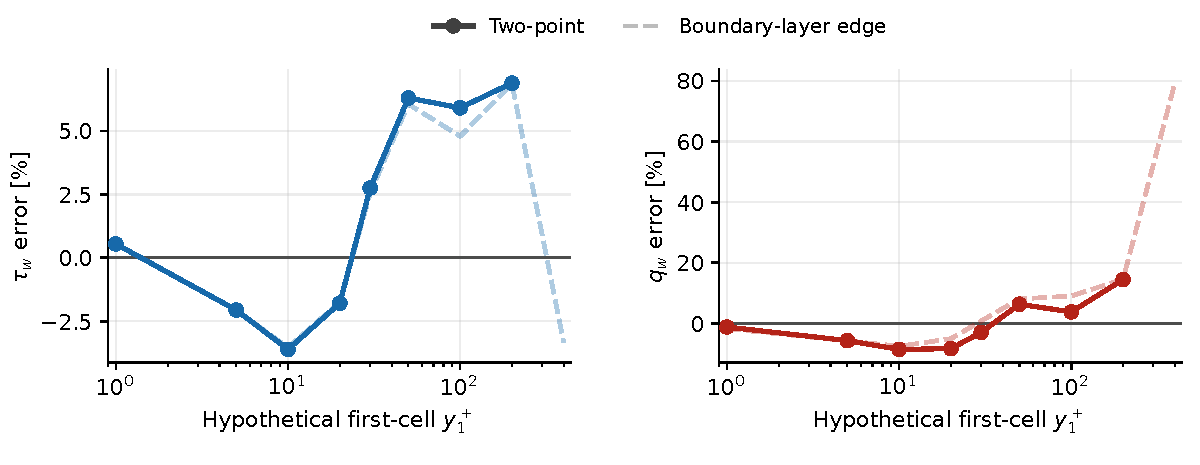
\includegraphics[width=\linewidth]{07_Error_Isolation_Results/Figures/Closures/a-priori_Li_M6Tw025.pdf}
    \caption[Li closure assessment on the M6Tw025 DNS profile]{A-priori Li wall-shear (left) and heat-flux (right) errors relative to the M6Tw025 DNS wall quantities. The solid curves use two virtual equal-height cells, with \(y_2=3y_1\); the dashed curves use a prescribed boundary layer-edge state. The horizontal coordinate is the virtual first-cell-centre height in DNS wall units. Each point is a separate inverse closure solution on the same prescribed profile.}
    \label{fig:wall-closure:a-priori-Li-M6Tw025}
\end{figure}

\begin{figure}[H]
    \centering
    % Figure provenance (WSL; absolute paths):
    %   Figure: /home/mgnadlinger/OpenFOAM/mgnadlinger-v2412/src/GriffinWallFunctions/tests/ReverseSolver/M6Tw025_Stat_Zhang/wall_flux_errors_vs_yplus.png
    %   Python script:
    %     /home/mgnadlinger/OpenFOAM/mgnadlinger-v2412/src/GriffinWallFunctions/tests/ReverseSolver/analyze_griffin_wall_function_profile_Zhang.py
    %   Data / simulation roots (high-level):
    %     /home/mgnadlinger/OpenFOAM/mgnadlinger-v2412/src/GriffinWallFunctions/tests/ReverseSolver/M6Tw025_Stat_Zhang
    %     /home/mgnadlinger/OpenFOAM/mgnadlinger-v2412/src/GriffinWallFunctions/tests/ReverseSolver
    %     /home/mgnadlinger/Zhang_DNS_ZPGFP/References/Data
    %   Note: The staged DNS input in ReverseSolver includes added Cf/Ch header fields; its DNS profile rows
    %     match References/Data.
    %   Thesis replot: Figures/Closures/plot_apriori_assessments.py; byte-for-byte
    %     saved sweeps and original paths/hashes in Figures/Closures/apriori_sources/.
    %   Layout: shear left, heat flux right; original 10.5 pt plot font retained.
    % End figure provenance.
    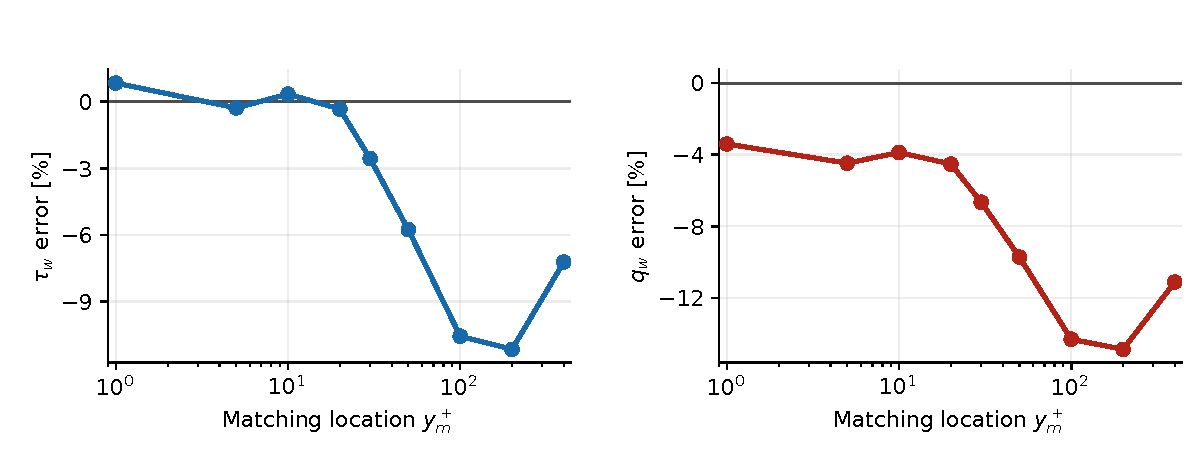
\includegraphics[width=\linewidth]{07_Error_Isolation_Results/Figures/Closures/a-priori_Griffin_M6Tw025.pdf}
    \caption[Griffin closure assessment on the M6Tw025 DNS profile]{A-priori Griffin wall-shear (left) and heat-flux (right) errors relative to the M6Tw025 DNS wall quantities. The prescribed DNS edge state remains fixed while the virtual matching height \(y_m^+\) is varied. Points above \(y_m=0.3\delta_{99}\), corresponding here to \(y_m^+\simeq134.6\), extend the assessment beyond the matching height used in the published a-priori comparison and are retained as sensitivity results.}
    \label{fig:wall-closure:a-priori-Griffin-M6Tw025}
\end{figure}

\clearpage

\begin{figure}[H]
    \centering
    % Figure provenance (WSL; absolute paths):
    %   Figure: /home/mgnadlinger/OpenFOAM/mgnadlinger-v2412/src/LiWallFunctions/tests/ReverseSolver/LowH_M3_Duan_Li/wall_flux_errors_vs_yplus.png
    %   Python scripts:
    %     /home/mgnadlinger/OpenFOAM/mgnadlinger-v2412/src/LiWallFunctions/tests/ReverseSolver/plot_m6tw025_flux_reference_overlay.py
    %     /home/mgnadlinger/OpenFOAM/mgnadlinger-v2412/src/LiWallFunctions/tests/ReverseSolver/analyze_li_wall_function_profile_Duan.py
    %   Data / simulation roots (high-level):
    %     /home/mgnadlinger/OpenFOAM/mgnadlinger-v2412/src/LiWallFunctions/tests/ReverseSolver/LowH_M3_Duan_Li
    %     /home/mgnadlinger/OpenFOAM/mgnadlinger-v2412/src/LiWallFunctions/tests/ReverseSolver/LowH_M3_Duan_Li_boundaryLayerEdge
    %     /home/mgnadlinger/OpenFOAM/mgnadlinger-v2412/src/LiWallFunctions/tests/ReverseSolver/LowH_M3_Duan
    %     /home/mgnadlinger/Duan_DNS_ZPGFP/Martin_Duan_Part4/SA_Prt0p9/LowH_M3
    %   Note: Closure input is the wall-resolved SA profile at time 20000.
    %   Note: The plot combines the second-cell and boundary-layer-edge a-priori sweep directories.
    %   Thesis replot: Figures/Closures/plot_apriori_assessments.py; byte-for-byte
    %     saved sweeps and original paths/hashes in Figures/Closures/apriori_sources/.
    %   Layout: shear left, heat flux right; original 10.5 pt plot font retained.
    % End figure provenance.
    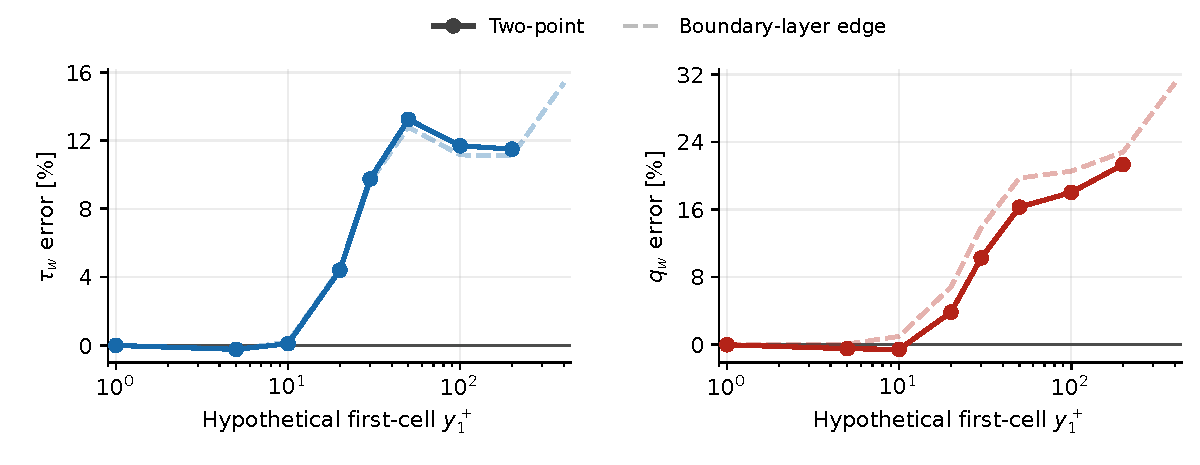
\includegraphics[width=\linewidth]{07_Error_Isolation_Results/Figures/Closures/a-priori_Li_LowHM3.pdf}
    \caption[Li closure assessment on the LowH\_M3 wall-resolved profile]{A-priori Li wall-shear (left) and heat-flux (right) errors relative to the wall-resolved SA baseline for LowH\_M3. Solid curves use the two-point formulation, with \(y_2=3y_1\), and dashed curves use the prescribed \(0.99U_\infty\) edge state. Sampling heights are expressed in wall units of the unchanged SA reference profile. These are closure errors relative to RANS, rather than errors relative to DNS.}
    \label{fig:wall-closure:a-priori-Li-LowHM3}
\end{figure}

\begin{figure}[H]
    \centering
    % Figure provenance (WSL; absolute paths):
    %   Figure: /home/mgnadlinger/OpenFOAM/mgnadlinger-v2412/src/GriffinWallFunctions/tests/ReverseSolver/LowH_M3_Duan/wall_flux_errors_vs_yplus.png
    %   Python script:
    %     /home/mgnadlinger/OpenFOAM/mgnadlinger-v2412/src/GriffinWallFunctions/tests/ReverseSolver/analyze_griffin_wall_function_profile_Duan_Part4.py
    %   Data / simulation roots (high-level):
    %     /home/mgnadlinger/OpenFOAM/mgnadlinger-v2412/src/GriffinWallFunctions/tests/ReverseSolver/LowH_M3_Duan
    %     /home/mgnadlinger/Duan_DNS_ZPGFP/Martin_Duan_Part4/SA_Prt0p9/LowH_M3
    %   Note: Closure input is the wall-resolved SA profile at time 20000.
    %   Thesis replot: Figures/Closures/plot_apriori_assessments.py; byte-for-byte
    %     saved sweeps and original paths/hashes in Figures/Closures/apriori_sources/.
    %   Layout: shear left, heat flux right; original 10.5 pt plot font retained.
    % End figure provenance.
    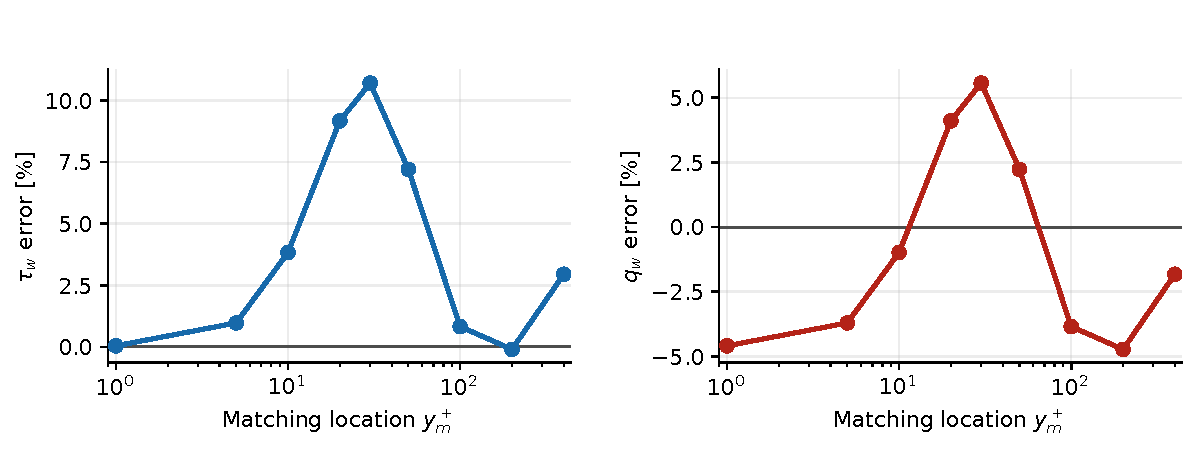
\includegraphics[width=\linewidth]{07_Error_Isolation_Results/Figures/Closures/a-priori_Griffin_LowHM3.pdf}
    \caption[Griffin closure assessment on the LowH\_M3 wall-resolved profile]{A-priori Griffin wall-shear (left) and heat-flux (right) errors relative to the wall-resolved SA baseline for LowH\_M3. The edge state is reconstructed once from the resolved profile using the Griffin boundary layer criterion, then held fixed while the virtual matching height is varied. The point at \(y_m^+=400\) lies above \(0.3\delta_{99}\) of this reconstructed boundary layer and is included as a sensitivity result.}
    \label{fig:wall-closure:a-priori-Griffin-LowHM3}
\end{figure}

\clearpage

\subsection{Influence of the prescribed RANS profile}
\label{subsec:erriso:rans-profile-influence}

In the previous Section\ref{sec:comparative:zpg:wall-resolved-baselines}, with the assessment of turbulence models, the wall-resolved M6Tw025 comparison in Figure~\ref{fig:wall-resolved:M6Tw025_BL_Profile} revealed a clear discrepancy in the temperature maximum and \(T(U)\) relation compared to the DNS reference. To quantify the consequence of this short coming of the turbulence models to the wall function closure that rely on these profiles, the Li et al. closure is evaluated on both the DNS profile and the wall-resolved SA profile at \(Pr_t=0.9\) and subsequently compared.
\par\medskip

Figure~\ref{fig:wall-closure:Li-M6Tw025-profile-influence} expresses both a-priori solved results relative to the same DNS wall quantities. Replacing the DNS profile as input, with the wall-resolved SA profile, changes the heat-flux prediction substantially, while the shear predictions remain much closer. This aligns with the SA velocity profile matching the DNS reference (see Figure~\ref{fig:wall-resolved:M6Tw025_BL_Profile} bottom right), while the \(T(U)\) profile, which feeds the wall function's energy closure, does not (see Figure~\ref{fig:wall-resolved:M6Tw025_BL_Profile} top left). At \(y_{1,\mathrm{DNS}}^+=30\), the predicted heat-flux increases by \(13.4\%\) relative to the DNS-input prediction, but shear changes by only \(0.1\%\). At \(y_{1,\mathrm{DNS}}^+=100\), the heat-flux error relative to DNS rises from \(+3.2\%\) to \(+16.0\%\). Thus, the thermal-profile discrepancy observed in the resolved calculation has a significant counterpart in the wall-function response, even where the velocity profiles appear convincing, and need to be addressed in future improvements of the turbulence models. In a fully coupled turbulence model + wall function CFD run, this error does not isolated as cleanly as in the a-priori solver here, because of the feedback of the wall function's wall quantity prediction into the overall flow field, but the underlying discrepancy still stands.

\begin{figure}[H]
    \centering
    % Figure provenance (WSL; absolute paths):
    %   Original figure: /home/mgnadlinger/OpenFOAM/mgnadlinger-v2412/src/LiWallFunctions/tests/ReverseSolver/M6Tw025_TM_closure_isolation/wall_flux_comparison.png
    %   Analysis script: /home/mgnadlinger/OpenFOAM/mgnadlinger-v2412/src/LiWallFunctions/tests/ReverseSolver/M6Tw025_TM_closure_isolation/run_comparison.py
    %   Saved data: /home/mgnadlinger/OpenFOAM/mgnadlinger-v2412/src/LiWallFunctions/tests/ReverseSolver/M6Tw025_TM_closure_isolation/comparison.csv
    %   Wall references: /home/mgnadlinger/OpenFOAM/mgnadlinger-v2412/src/LiWallFunctions/tests/ReverseSolver/M6Tw025_TM_closure_isolation/reference_states.csv
    %   Original DNS input: /home/mgnadlinger/Zhang_DNS_ZPGFP/References/Data/M6Tw025_Stat.dat
    %   Original SA input: /home/mgnadlinger/Zhang_DNS_ZPGFP/SA_Prt0p9/M6Tw025/postProcessing/TM_ZPGFP/15000/profile_Re_delta2.csv
    %   Thesis export script: thesis/07_Error_Isolation_Results/Figures/Closures/plot_tm_profile_closure.py
    %   Note: The earlier thesis PNG retained only the original figure's middle row,
    %     omitting its legend. Re-exported from saved CSVs with a shared legend;
    %     both panels retain the common DNS denominator and all eight heights.
    %   Note: Fixed omegaH=0.72; each input retains its native wall state.
    %     This is a complete-profile comparison, not a temperature-only swap.
    % End figure provenance.
    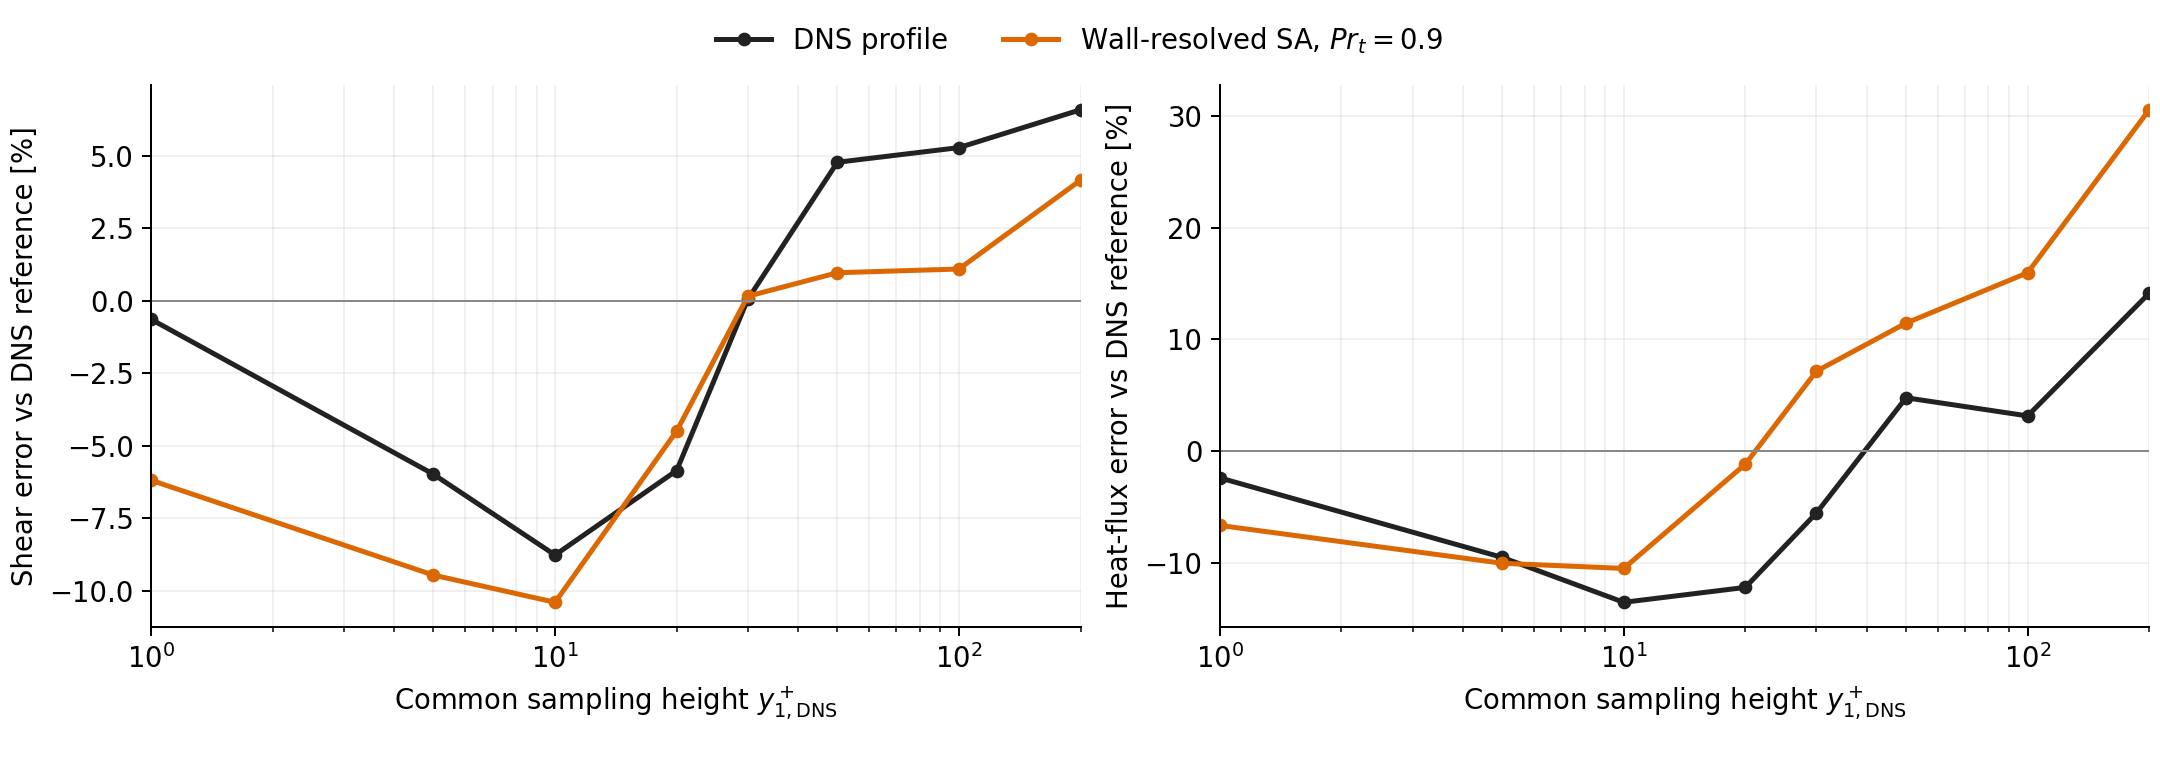
\includegraphics[width=\linewidth]{07_Error_Isolation_Results/Figures/Closures/TM_prof_err_Li-aprio.png}
    \caption[Effect of DNS and SA inputs on the M6Tw025 Li closure]{Li closure evaluated on the M6Tw025 DNS and wall-resolved SA profiles. Left: wall-shear error; right: heat-flux error. Both curves use the DNS wall heat-flux and shear stress as their reference, hence the orange line not converging to zero error at \(y_{1,\mathrm{DNS}}^+=1\). The virtual sampling heights of \(y_1\) and \(y_2=3y_1\) are identical for both inputs; the abscissa uses the supplied DNS wall units.}
    \label{fig:wall-closure:Li-M6Tw025-profile-influence}
\end{figure}

The common DNS denominator in the figure must be distinguished from recovery of each profile's own wall flux. Over e.g. the three sampled heights \(y_{1,\mathrm{DNS}}^+=30\), \(50\) and \(100\), the mean absolute heat-flux error relative to the corresponding source wall value increases from \(4.5\%\) for DNS inputs to \(17.8\%\) for SA inputs. The discrepancy is therefore more than the offset between the resolved SA and DNS wall fluxes itself, hence the discrepancy in the wall-resolved boundary layer to the DNS impacts the wall function closure's accuracy. 
\par\medskip

This is also clearly seen through the immediate mechanism, which is the inferred enthalpy--velocity wall slope in the wall function's energy closure. Li's generalized recovery enthalpy is obtained from
\begin{equation}
    h_{rg}
    =\frac{h_1-h_w(1-r)-h_Rr^2}{r(1-r)},
    \qquad r=\frac{U_1}{U_R},
    \label{eq:erriso:li-reference-inversion}
\end{equation}
where \((U_R,h_R)\) is the reference state, here the second sampling point~\cite[Eq.~(40)]{li2025WF}.

With positive heat-transfer into the cooled wall denoted by \(Q_w=|q_w|\), Li's relations give
\begin{equation}
    S=\left.\frac{\mathrm{d}h}{\mathrm{d}U}\right|_w
      =\frac{h_{rg}-h_w}{U_2},
    \qquad Q_w=\frac{\tau_w S}{Pr_w},
    \label{eq:erriso:li-profile-wall-slope}
\end{equation}
where \(h_{rg}\) follows from Equation~\eqref{eq:erriso:li-reference-inversion}~\cite[Eqs.~(40)--(41)]{li2025WF}. At \(y_{1,\mathrm{DNS}}^+=30\), changing from DNS to SA inputs raises \(S\) by \(13.3\%\), accounting for almost all of the heat-flux increase while the recovered shear is nearly unchanged because so is the sampled velocity profile. This identifies the thermal wall slope as the immediate route through which the profile mismatch affects the predicted heating. Thus future improvements to RANS turbulence models should not only improve the heat-flux and shear stress results in isolation, but also need to tackle the challenge in hypersonic cold-wall boundary layer reproducibility. 

\subsection{Summary and Implications for the coupled assessment}
The a-priori assessment (ref. Section~\ref{subsec:erriso:apriori-results}) identifies appreciable baseline errors in both closures, even when the sampled inputs are supplied from known reference profiles. However, neither formulation shows a systematic breakdown in the buffer layer. The results therefore provide no basis for excluding a buffer-layer sampling interval because of the blending between the viscous and logarithmic relations. But the remaining closure errors do warrant investigation into better, improved velocity transformations and closure theories.
\par\medskip

A comparison of supplying the a-priori solver with the DNS or the wall-resolved SA profile (ref. Section~\ref{subsec:erriso:rans-profile-influence}) identifies a further limitation: discrepancies in the wall-resolved RANS profile (as identified in Section~\ref{subsec:comparative:zpg:wr-profiles}) can substantially alter the wall-function heat-flux prediction. In the example of the Li assessment on the M6Tw025 case, it shows that a convincing velocity profile does not compensate for an inaccurate \(T(U)\) relation, which changes the inferred thermal wall slope. Improving the coupled prediction therefore requires attention to both the closure's baseline accuracy and the turbulence model's reproduction of the cold-wall thermal profile. These findings provide the context for the following assessment of the additional influence of spatial discretization in Section~\ref{subsec:comparative:zpg:yplus-sensitivity}, especially with the final isolation from the closure error by overwriting the closure theory with a fitted function in Section~\ref{subsec:comparative:zpg:fitted-closure}.

\section{Wall-function in FVM CFD: Spatial-discretization error and sampling sensitivity}
\label{subsec:comparative:zpg:yplus-sensitivity}

The closure assessment in Section~\ref{sec:comparative:zpg:cross-comparison} determines how accurately a wall function recovers wall loads from a prescribed, ideal, boundary layer state. In CFD, that state is itself part of a discrete solution. Consequently, a change in sampling height can alter both the closure response and the numerical solution of the surrounding boundary layer. This section analysis the behaviour of the wall functions on the LowH\_M3 and M6Tw025 cases, by first examining their accuracy and consistency on a conventional mesh strategy as the wall functions were intended to be used e.g. by Li et al. in \cite{li2025WF}. Subsequently, a novel boundary layer-informed mesh design is introduced to isolate the identified internal-face discretization errors. Finally the, in the previous section identified, closure discrepancies are revisited in the context of the new meshes, by presccribing an ideally fitted closure to isolate out all found error effects, but from the turbulence models.

\subsection{Wall functions on conventional meshes}
\label{subsec:comparative:zpg:conventional-mesh}

The conventional mesh strategy and sampling geometry are introduced in Section~\ref{subsec:wall-functions:sampling-geometry}. The general idea how conventionally meshes for wall-functions are designed is, to increase the first-cell height until the desired \(y^+_1\) is achieved. In these \textit{conventional wall-function mesh} sweeps, increasing the physical first-cell height moves the wall-function sample outward and increases the separation of neighbouring cell centres. Thus, on \textit{conventional wall-function mesh} the sampling location $y_s^+$ coincides with the first-cell location $y_1^+$, while the spacing of internal-face stencils, herin referred to as \(h^+\),  changes with it (see Figure~\ref{fig:WF:exemplaray_y+10_mesh} \(h^+\) change between exemplary \(y^+_1 = 10\) and \(y^+_1 = 30\) meshes). One should keep in mind, that the sample height $y_s^+$ and physical first-cell mesh resolution \(y^+_1\) need not necessarily be identical, but one could also take the second off-wall cell centre as the wall function sampling point. This distinction becomes essential when the two are varied independently below.
\par\medskip

Figure~\ref{fig:WF:mesh} shows a representative conventional M6Tw025 mesh with special attention to the leading edge region. The leading edge requires additional care because the local friction velocity and the boundary layer thickness differ substantially from their downstream values at which the sampling station with the desired \(y^+_1\) is specified. With a constant physical first-cell height, the elevated upstream shear raises $y_1^+$ significantly above its intended value at the comparison station. For coarse meshes it was found, that \(y^+_1\) at the leading edge region even spiked beyond values where the wall-function is applicable and resulted in unphyiscal behaviour which propagates downstream. Figure~\ref{fig:WF:mesh_constant_smooth} illustrates this effect and its reduction by smoothly increasing the first-cell height over the initial $80\,\mathrm{mm}$ of the plate, thus giving a clearer picture of the actual wall-function behaviour.

\begin{figure}[H]
    \centering
    % Figure provenance (WSL; absolute paths):
    %   Figure: /mnt/c/Users/MichaelGnadlinger/OneDrive - Hypersonica/Hypersonica Team - Documents/02 Technical/03 Flight physics/16 Theses/2026/01 Gnadl/Docs_and_Presentations/Thesis_tex/thesis/07_Error_Isolation_Results/Figures/WallFunctions/M6Tw025_y+_100_mesh.png
    %   Python script: Not applicable: direct mesh-view screenshot (confirmed by author).
    %   Data / simulation roots (high-level):
    %     /home/mgnadlinger/Xue_et_al/flat_plate/M6Tw025
    %     /home/mgnadlinger/Xue_et_al/flat_plate/M6Tw025/Li_SA/100_1p5
    %   Note: No separate export file or plotting script: retained screenshot is at the figure path above.
    %   Note: M6Tw025 wall-function mesh with nominal y+ approximately 100. Li_SA/100_1p5 is a corresponding
    %     available case; the original GUI case path was not recorded.
    % End figure provenance.
    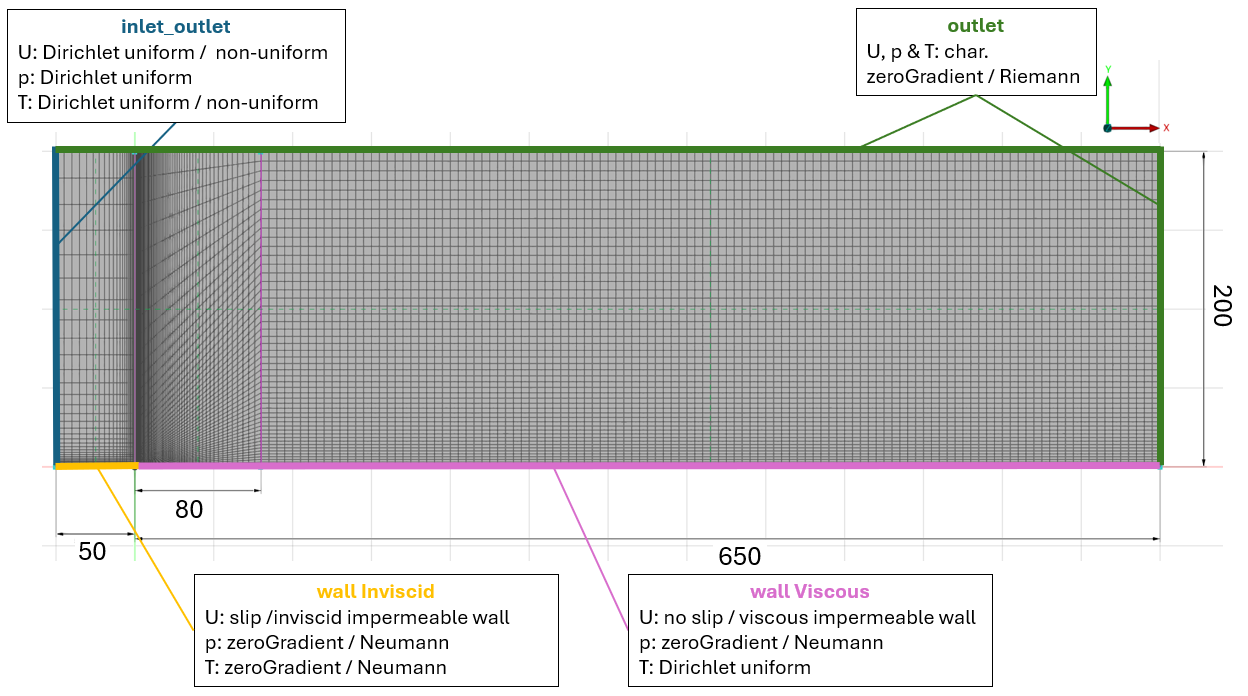
\includegraphics[width=\linewidth,height=.62\textheight,keepaspectratio]{07_Error_Isolation_Results/Figures/WallFunctions/M6Tw025_y+_100_mesh.png}
    \caption{Conventional wall-function mesh for M6Tw025 with nominal first-cell location $y_1^+\approx100$ at the comparison station. Streamwise refinement and a smaller first-cell height resolve the leading-edge region; the wall-normal spacing increases smoothly over the first $80\,\mathrm{mm}$.}
    \label{fig:WF:mesh}
\end{figure}

\begin{figure}[H]
    \centering
    % Figure provenance (WSL; absolute paths):
    %   Figure: /mnt/c/Users/MichaelGnadlinger/OneDrive - Hypersonica/Hypersonica Team - Documents/02 Technical/03 Flight physics/16 Theses/2026/01 Gnadl/Docs_and_Presentations/Thesis_tex/thesis/07_Error_Isolation_Results/Figures/WallFunctions/y+_40_M6Tw025_LiWF_constant.png
    %   Python script: Not applicable: direct ParaView postprocessing screenshot (confirmed by author).
    %   Data / simulation roots (high-level):
    %     /home/mgnadlinger/Xue_et_al/flat_plate/legacy/M6Tw025/LiNeumann_6e-1
    %   Note: No separate export file or plotting script: retained screenshot is at the figure path above.
    %   Note: Association with the listed legacy Li case is inferred from matching mesh geometry and wall-y+
    %     distribution; the original ParaView case path was not recorded.
    % End figure provenance.
    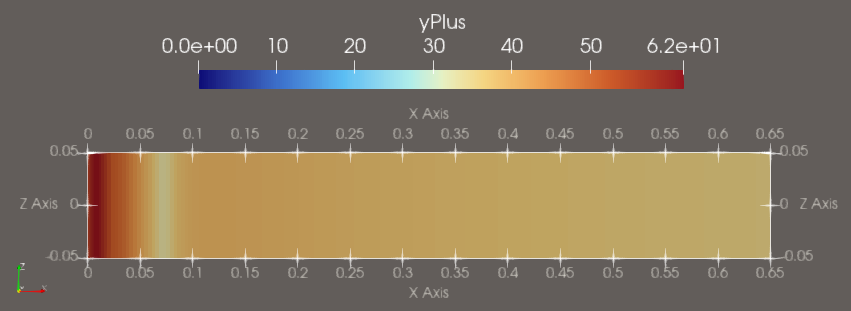
\includegraphics[width=0.7\linewidth,height=.30\textheight,keepaspectratio]{07_Error_Isolation_Results/Figures/WallFunctions/y+_40_M6Tw025_LiWF_constant.png}
    \par\medskip
    % Figure provenance (WSL; absolute paths):
    %   Figure: /mnt/c/Users/MichaelGnadlinger/OneDrive - Hypersonica/Hypersonica Team - Documents/02 Technical/03 Flight physics/16 Theses/2026/01 Gnadl/Docs_and_Presentations/Thesis_tex/thesis/07_Error_Isolation_Results/Figures/WallFunctions/y+_40_M6Tw025_LiWF_smooth.png
    %   Python script: Not applicable: direct ParaView postprocessing screenshot (confirmed by author).
    %   Data / simulation roots (high-level):
    %     /home/mgnadlinger/Xue_et_al/flat_plate/legacy/M6Tw025/LiNeumann_6e-1_smooth
    %   Note: No separate export file or plotting script: retained screenshot is at the figure path above.
    %   Note: Association with the listed legacy Li case is inferred from matching mesh geometry and wall-y+
    %     distribution; the original ParaView case path was not recorded.
    % End figure provenance.
    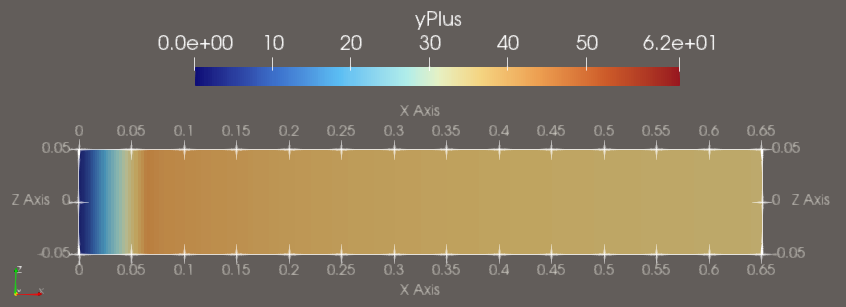
\includegraphics[width=0.7\linewidth,height=.30\textheight,keepaspectratio]{07_Error_Isolation_Results/Figures/WallFunctions/y+_40_M6Tw025_LiWF_smooth.png}
    \caption{Wall-unit first-cell location along the M6Tw025 plate for a nominal $y_1^+\approx40$ Li wall-function mesh. A constant physical first-cell height (top) produces elevated $y_1^+$ near the leading edge. A smooth increase of first-cell height over the first $80\,\mathrm{mm}$ (bottom) reduces this upstream excursion.}
    \label{fig:WF:mesh_constant_smooth}
\end{figure}

Figures~\ref{fig:WF:Li-LowHM3_conventional_mesh}--\ref{fig:WF:Griffin-M6Tw025_conventional_mesh} show the resulting wall heat-flux and shear-stress errors. All curves use the signed relative error to the respective DNS reference at the matched \(Re_{\delta2}\) station (see Section~\ref{subsec:evaluation:matching-station}). The dashed lines show the wall-resolved SA result at the same station as presented and discussed in Section~\ref{sec:comparative:zpg:wall-resolved-baselines}. Around the DNS reference value for th heat-flux and shear stress, the shading marks a $\pm5\%$ error band (as selected in Section~\ref{sec:evaluation:success-criteria}). The horizontal axis shows the actual, calculated first-cell $y_1^+$ at the matched station on these conventional meshes, so each point represents a different CFD simulation with the only change being the first-cell height in the sampling region of the used mesh.
\par\medskip

From Figures~\ref{fig:WF:Li-LowHM3_conventional_mesh}--\ref{fig:WF:Griffin-M6Tw025_conventional_mesh}  it is immediatly visible that the wall-function results are highly sensitive to the first-cell height. But the errors are not monotonic with increasing $y_1^+$, but instead exhibit a pronounced different behaviour in the sublayer region, the buffer and the log-layer region of the cases. The wall-function error bands are also substantially larger than the corresponding a-priori closure variations identified in Section~\ref{subsec:erriso:apriori-results}. Griffin gives signed shear-stress errors of approximately \(-20\%\) to \(+8\%\) and heat-flux errors of \(-16\%\) to \(+12\%\). Over the same cases and sampling-height interval, the Li wall function gives respective shear-stress errors of approximately \(-7\%\) to \(+14\%\) and heat-flux errors of \(-6\%\) to \(+27\%\). But for an engineering context, the high sensitivity of the wall-function results to the first-cell height is arguably more concerning than the absolute error magnitude because it introduces a substantial uncertainty and not a clear bias.
\par\medskip

Looking at the sub-layer region, the wall-function results approach the wall-resolved baseline to within the closure accuracy as expected. Looking at Li's previously found closure behaviour where at \(y^+ = 1\) the wall-function closure error is basically zero (see a-priori result for M6Tw025 in Figure~\ref{fig:wall-closure:a-priori-Li-M6Tw025} and LowH\_M3 in Figure \ref{fig:wall-closure:a-priori-Li-LowHM3}), the wall-function CFD results are also very close to the wall-resolved baseline (see conventional mesh CFD result for M6Tw025 in Figure~\ref{fig:WF:Li-M6Tw025_conventional_mesh} and LowH\_M3 in Figure \ref{fig:WF:Li-LowHM3_conventional_mesh}). The same findings also apply to the Griffin wall-function results where for both cases the a-priori closure assessment in Section~\ref{subsec:erriso:apriori-results} shows a low-$y^+$ closure discrepancy of about $-5\%$ for the wall heat-flux (see a-priori result for M6Tw025 in Figure~\ref{fig:wall-closure:a-priori-Griffin-M6Tw025} and LowH\_M3 in Figure \ref{fig:wall-closure:a-priori-Griffin-LowHM3}), which is also reflected in the deviation of wall-function CFD results from the wall-resolved baseline (see conventional mesh CFD result for M6Tw025 in Figure~\ref{fig:WF:Griffin-M6Tw025_conventional_mesh} and LowH\_M3 in Figure \ref{fig:WF:Griffin-LowHM3_conventional_mesh}).
\par\medskip

Beyond the sublyer, reaching into the buffer layer, the wall-function CFD results do not follow this behaviour where the whole error can be explained through the closure error alone. Rather it is clear that the wall-function CFD results are not only affected by the closure discrepancy, but also by additional error sources. The cause for this behaviour beyond the sublayer is analysed and examined in the next step, where the internal-face fluxues of momentum and energy where compared to the wall-resolved results, and found in the spatial discretization.
\par\medskip

On the even higher $y^+$ conventional meshes, reaching the log-layer and beyond, a sharp reduction in the wall-function CFD error is observed. This reduction does not necessarily indicate a better wall-function performance, but rather indicates a different error sources, that happens to cancel some of the closure discrepancy. In Figure~\ref{fig:WF:Griffin-M6Tw025_conventional_mesh} for example the relative error becomes highly negative, instead of cancelling out to zero. And this behvior in the log-layer and beyond also, as in the buffer layer, do not follow the a-priori seen closure discrepancy. But it is a nice indication why Li et al  found a good agreement of their wall-function CFD results with the DNS reference, because for their validation cases they used a conventional mesh with a first-cell height of \(y^+_1 = 4, 8 \) and then for their cases comfortly in the log-layer \(y^+_1 = 104, 133, 156, 200\) \cite[Figures 17--20 and 23--24]{li2025WF}. Li et al. claim "[...] and it is also essential to avoid them [first grid points] falling into the bufferlayer when using the wall function method." \cite[p. 61]{li2025WF}. So in their analysis they avoided the regions with high sensitivity and large errors, but attributed it to the wrong cause. Griffin et al. use \(y_m=0.3\delta\) for their principal wall-flux comparisons, but also reduce the matching height during WMLES mesh refinement, reaching the buffer region in the lower-Reynolds-number channel case~\cite[Section~4.1]{griffin2023WF}. Their study therefore does not support a blanket exclusion of buffer-layer sampling. As discussed in Section~\ref{subsec:wall-functions:griffin:validation-scope}, those matching-height and LES-resolution studies differ from the present conventional RANS mesh sweeps.

\begin{figure}[H]
    \centering
    % Figure provenance (WSL; absolute paths):
    %   Figure: /home/mgnadlinger/WF_validation/LowH_M3/validation/outputs/plots/li_sa_dns_station_relative_error.png
    %   Python script:
    %     /home/mgnadlinger/WF_validation/LowH_M3/validation/scripts/plot_wall_flux_sweeps.py
    %   Data / simulation roots (high-level):
    %     /home/mgnadlinger/WF_validation/LowH_M3/Li_SA
    %     /home/mgnadlinger/WF_validation/LowH_M3/wall_resolved/SA/LowH_M3
    %     /home/mgnadlinger/WF_validation/LowH_M3/Digitizations
    %   Note: Thesis image removes the 128-pixel title strip from the source export.
    % End figure provenance.
    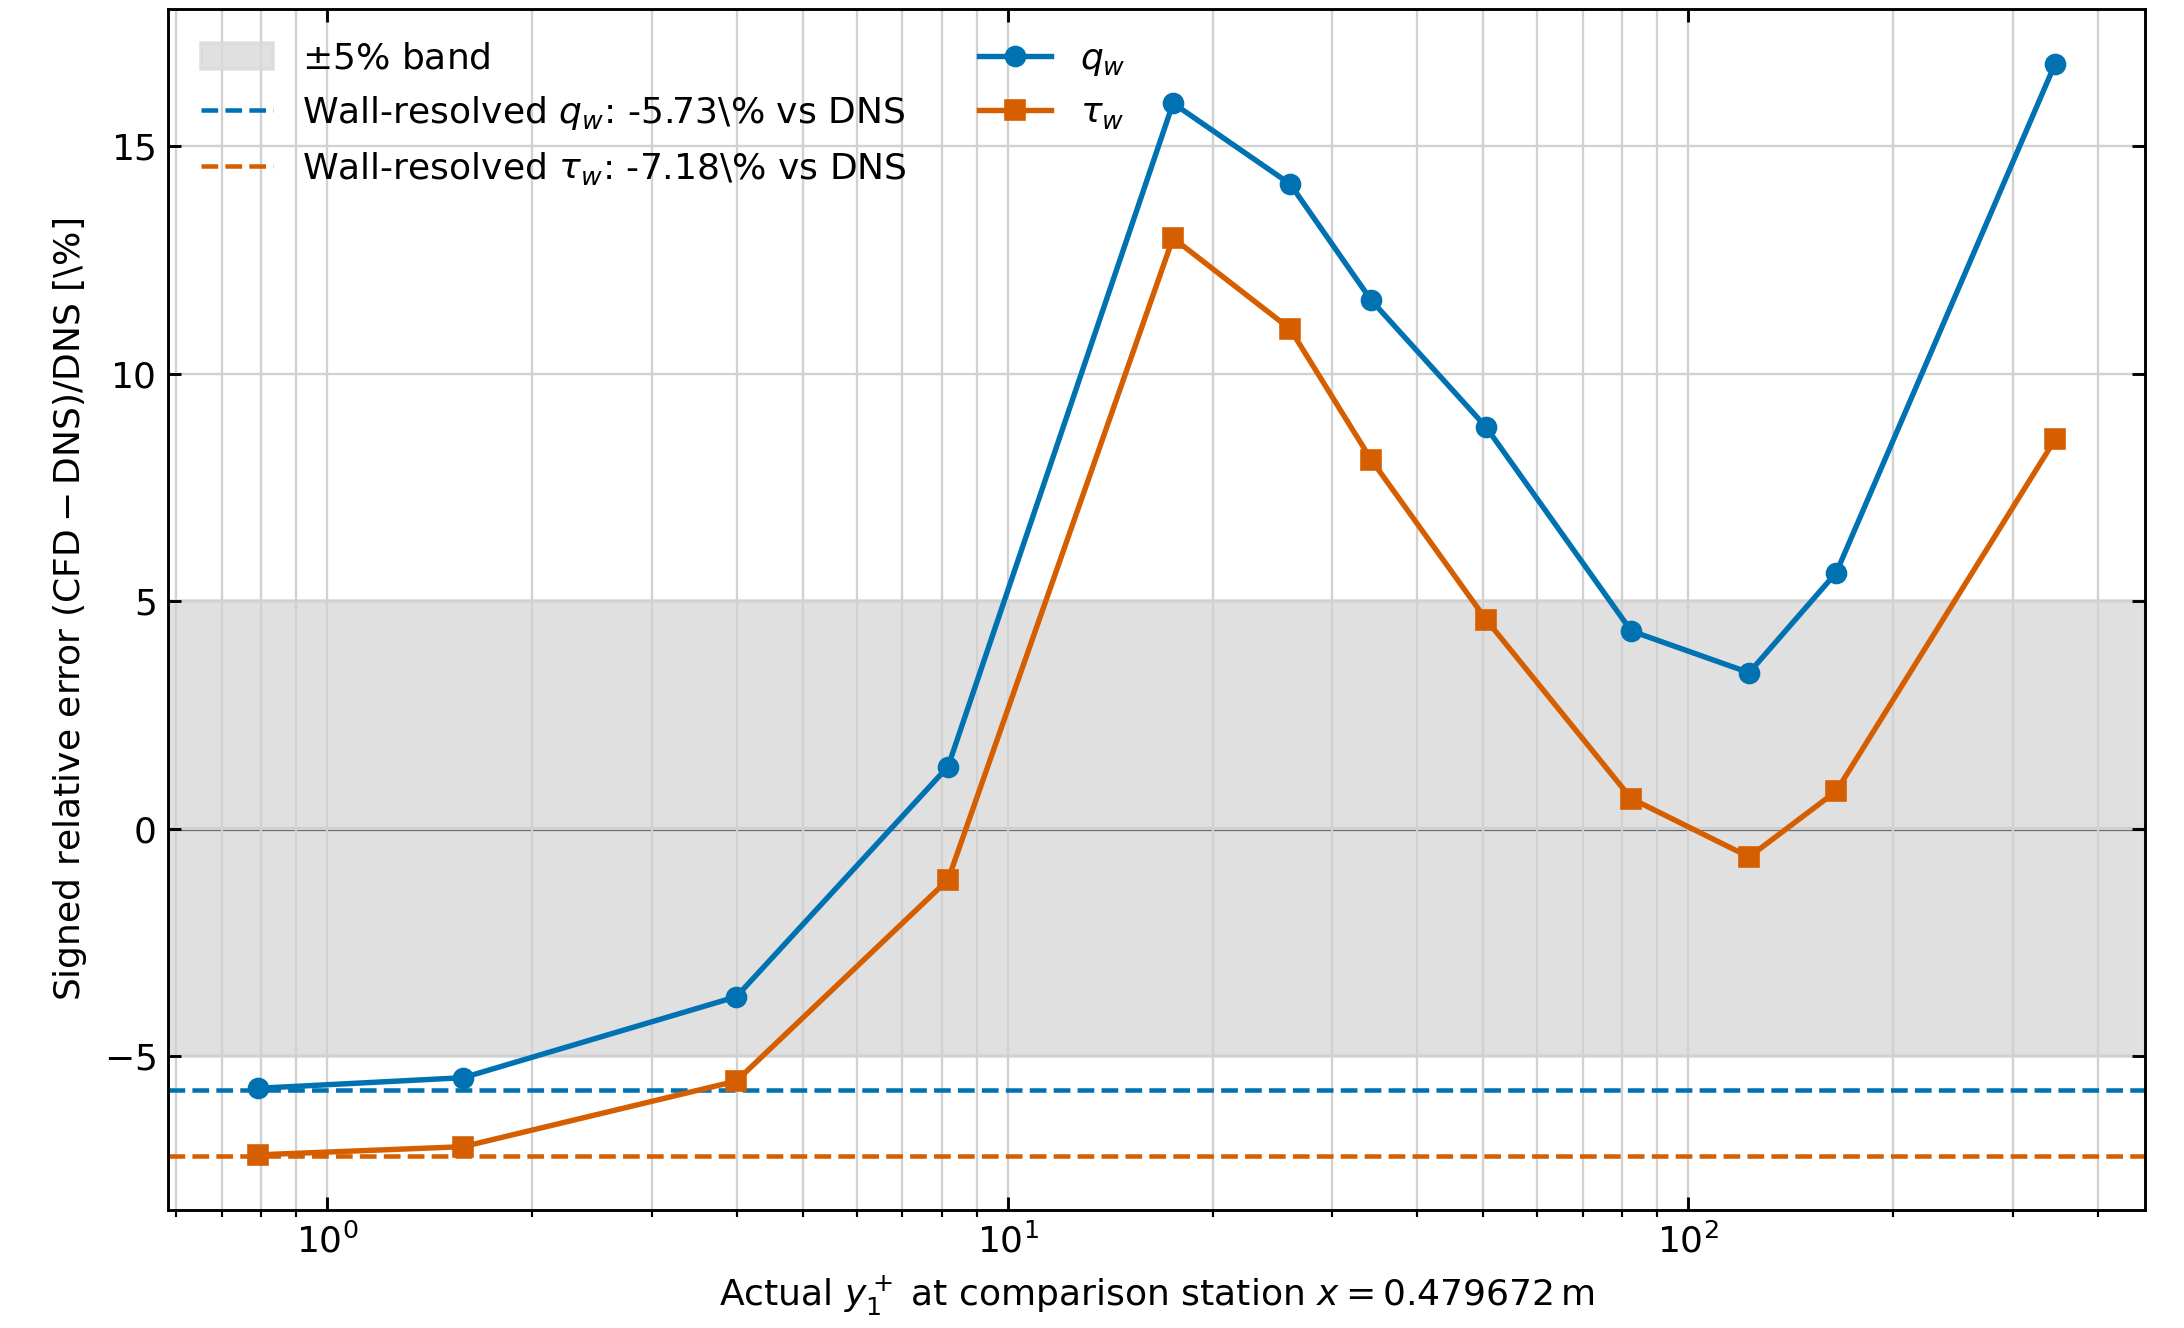
\includegraphics[width=\linewidth,height=.62\textheight,keepaspectratio]{07_Error_Isolation_Results/Figures/WallFunctions/04_ConvMesh_Li_LowHM3.png}
    \caption{Li wall-function CFD with SA on conventional meshes for LowH\_M3: signed errors in wall heat-flux $q_w$ and shear stress $\tau_w$ relative to DNS, evaluated at $x=0.479672\,\mathrm{m}$ against the actual first-cell $y_1^+$. Dashed lines denote the wall-resolved SA errors; shading marks $\pm5\%$ relative to DNS.}
    \label{fig:WF:Li-LowHM3_conventional_mesh}
\end{figure}

\begin{figure}[H]
    \centering
    % Figure provenance (WSL; absolute paths):
    %   Figure: /home/mgnadlinger/WF_validation/LowH_M3/validation/outputs/plots/griffin_sa_dns_station_relative_error.png
    %   Python script:
    %     /home/mgnadlinger/WF_validation/LowH_M3/validation/scripts/plot_wall_flux_sweeps.py
    %   Data / simulation roots (high-level):
    %     /home/mgnadlinger/WF_validation/LowH_M3/Griffin_SA
    %     /home/mgnadlinger/WF_validation/LowH_M3/wall_resolved/SA/LowH_M3
    %     /home/mgnadlinger/WF_validation/LowH_M3/Digitizations
    % End figure provenance.
    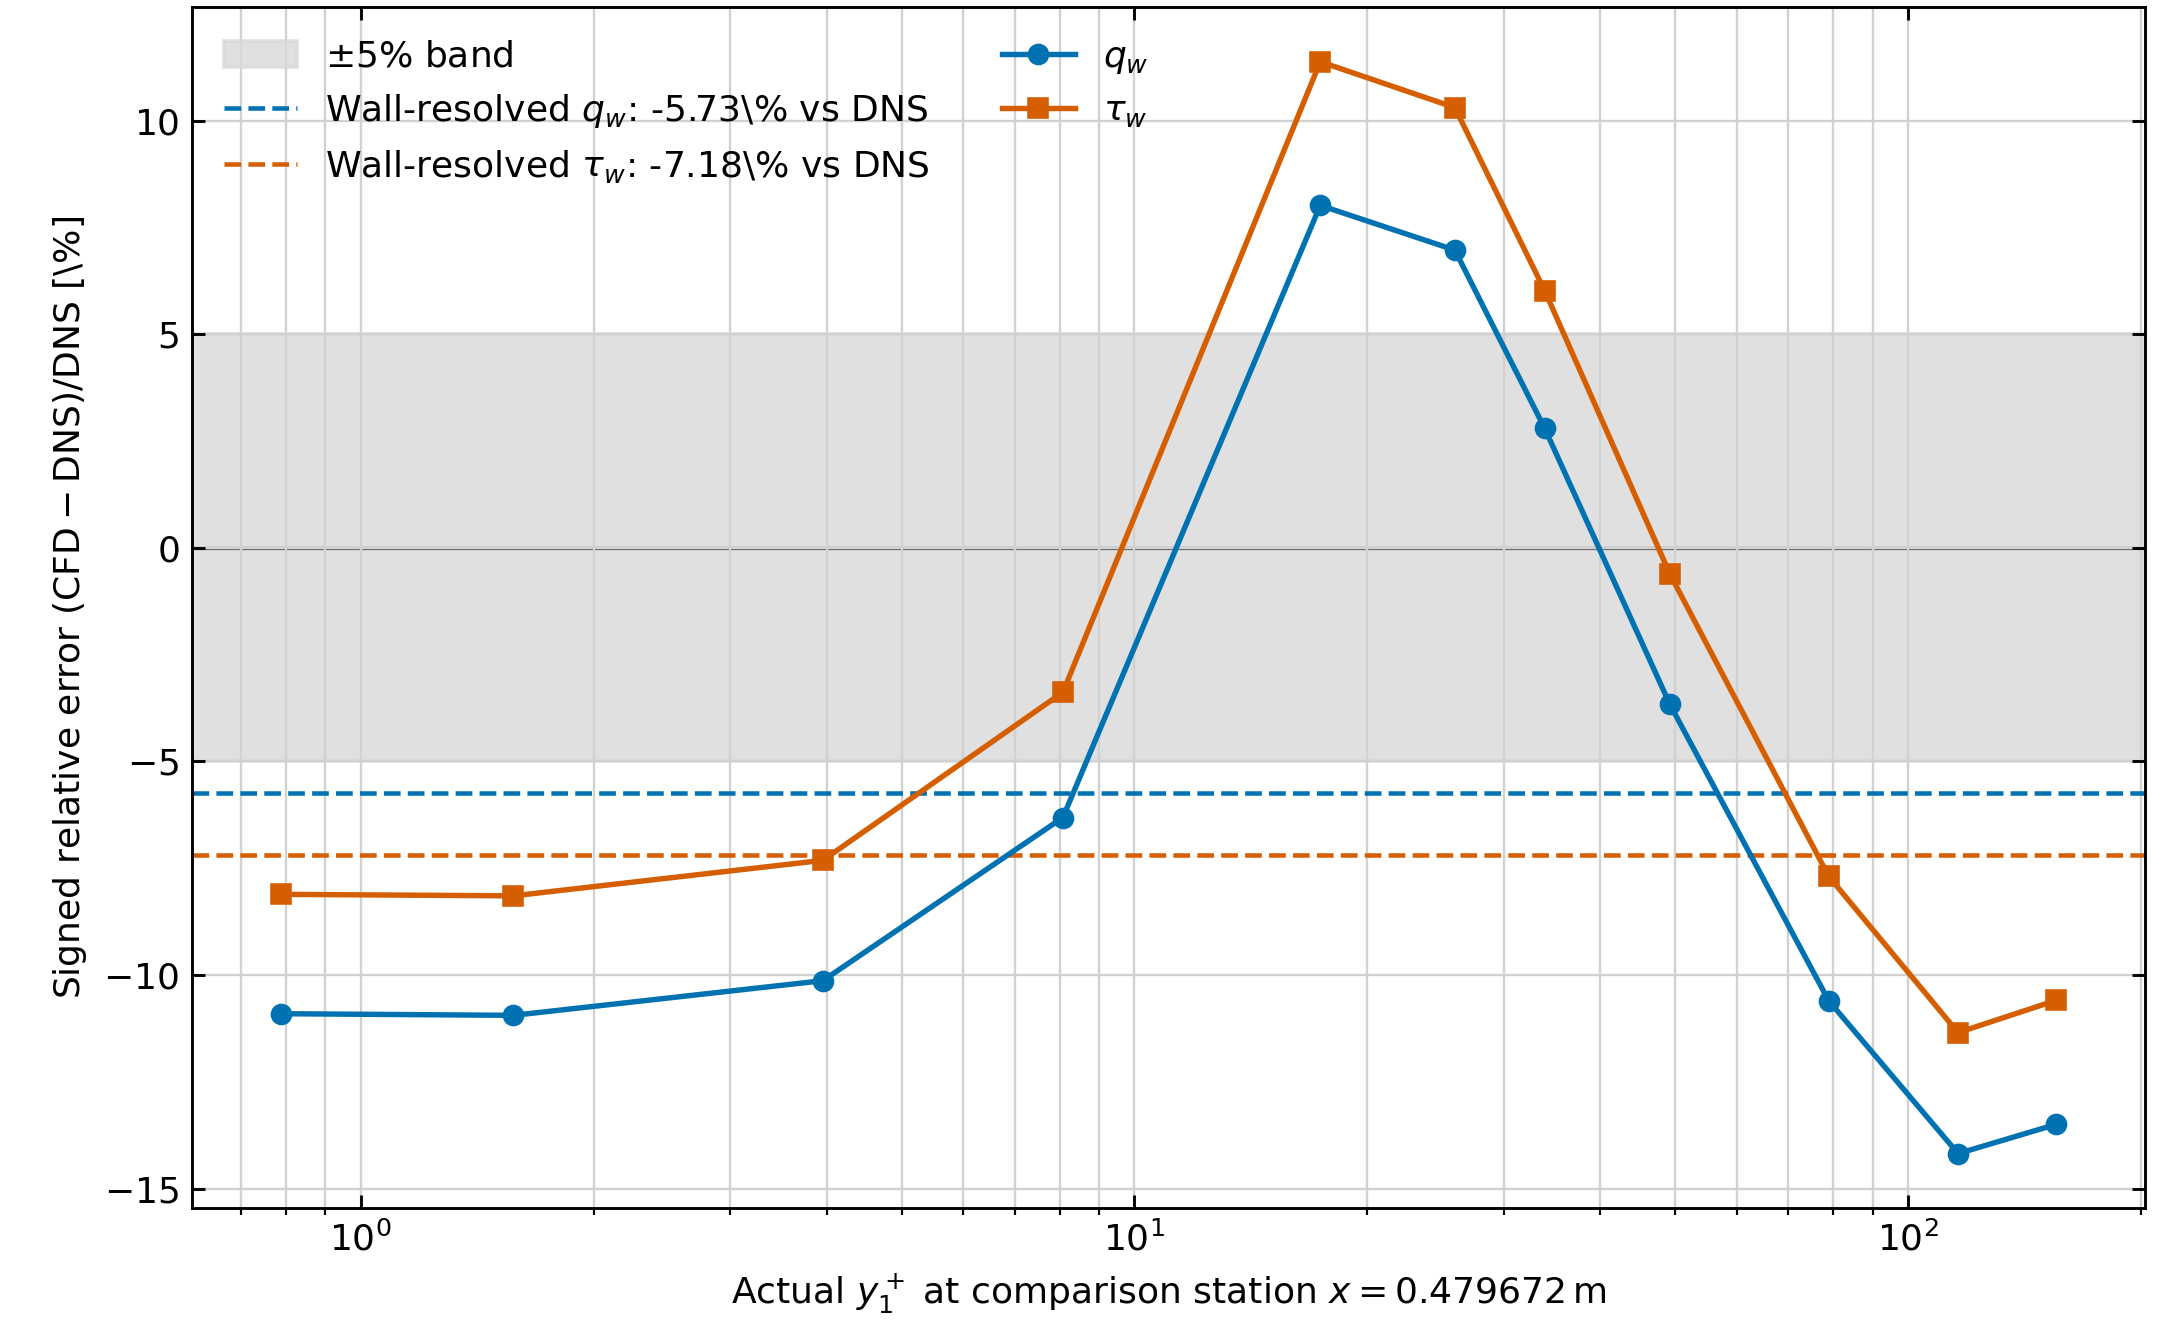
\includegraphics[width=\linewidth,height=.62\textheight,keepaspectratio]{07_Error_Isolation_Results/Figures/WallFunctions/04_ConvMesh_Griffin_LowHM3.png}
    \caption{Griffin wall-function CFD with SA on conventional meshes for LowH\_M3. Wall heat-flux and shear-stress errors use the same DNS normalization and comparison station as Figure~\ref{fig:WF:Li-LowHM3_conventional_mesh}. Dashed lines denote the wall-resolved baseline; shading marks $\pm5\%$ relative to DNS.}
    \label{fig:WF:Griffin-LowHM3_conventional_mesh}
\end{figure}

\begin{figure}[H]
    \centering
    % Figure provenance (WSL; absolute paths):
    %   Figure: /home/mgnadlinger/Xue_et_al/flat_plate/M6Tw025/validation/outputs_Li_SA/group1_wall_flux_relative_error_vs_yplus.png
    %   Python script:
    %     /home/mgnadlinger/Xue_et_al/flat_plate/M6Tw025/validation/plot_wall_fluxes_and_figure6.py
    %   Data / simulation roots (high-level):
    %     /home/mgnadlinger/Xue_et_al/flat_plate/M6Tw025/Li_SA
    %     /home/mgnadlinger/Xue_et_al/flat_plate/M6Tw025/Li_SA/SA_Prt0p9_baseline
    %     /home/mgnadlinger/Xue_et_al/flat_plate/M6Tw025/Digitizations
    %     /home/mgnadlinger/Zhang_DNS_ZPGFP/References/Data
    %   Note: Thesis image removes the 128-pixel title strip from the source export.
    % End figure provenance.
    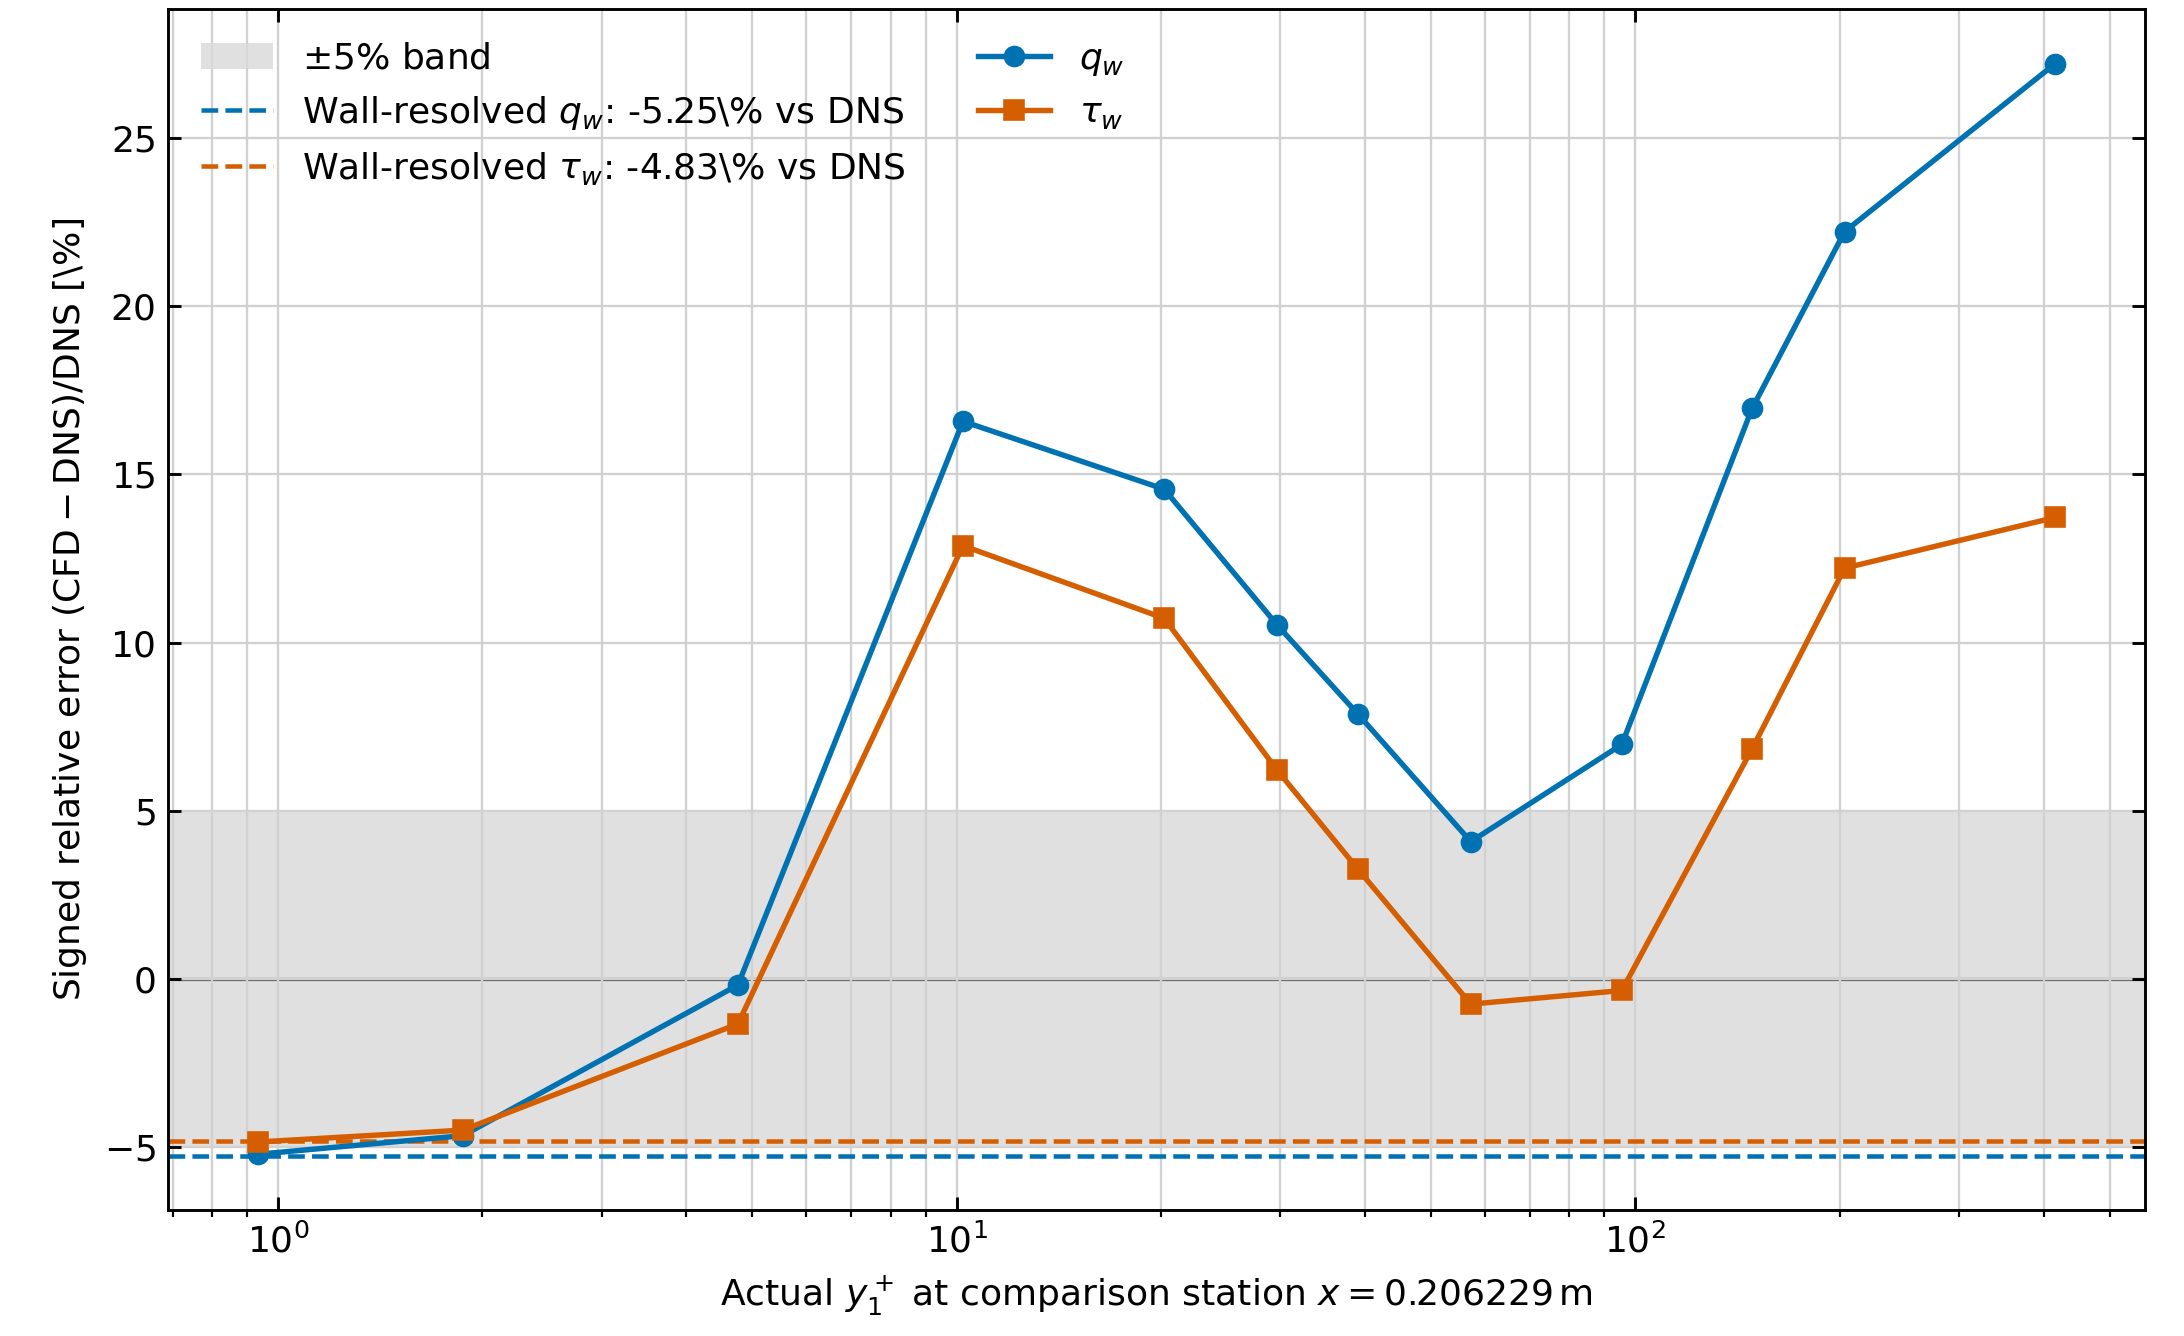
\includegraphics[width=\linewidth,height=.62\textheight,keepaspectratio]{07_Error_Isolation_Results/Figures/WallFunctions/04_ConvMesh_Li_M6Tw025.png}
    \caption{Li wall-function CFD with SA on conventional meshes for M6Tw025: signed wall heat-flux and shear-stress errors relative to DNS at $x=0.206229\,\mathrm{m}$ against the actual first-cell $y_1^+$. Dashed lines denote the wall-resolved SA errors; shading marks $\pm5\%$ relative to DNS.}
    \label{fig:WF:Li-M6Tw025_conventional_mesh}
\end{figure}

\begin{figure}[H]
    \centering
    % Figure provenance (WSL; absolute paths):
    %   Figure: /home/mgnadlinger/Xue_et_al/flat_plate/M6Tw025/validation/outputs_Griffin_SA/group1_wall_flux_relative_error_vs_yplus.png
    %   Python script:
    %     /home/mgnadlinger/Xue_et_al/flat_plate/M6Tw025/validation/plot_wall_fluxes_and_figure6.py
    %   Data / simulation roots (high-level):
    %     /home/mgnadlinger/Xue_et_al/flat_plate/M6Tw025/Griffin_SA
    %     /home/mgnadlinger/Xue_et_al/flat_plate/M6Tw025/Griffin_SA/SA_Prt0p9_baseline
    %     /home/mgnadlinger/Xue_et_al/flat_plate/M6Tw025/Digitizations
    %     /home/mgnadlinger/Zhang_DNS_ZPGFP/References/Data
    % End figure provenance.
    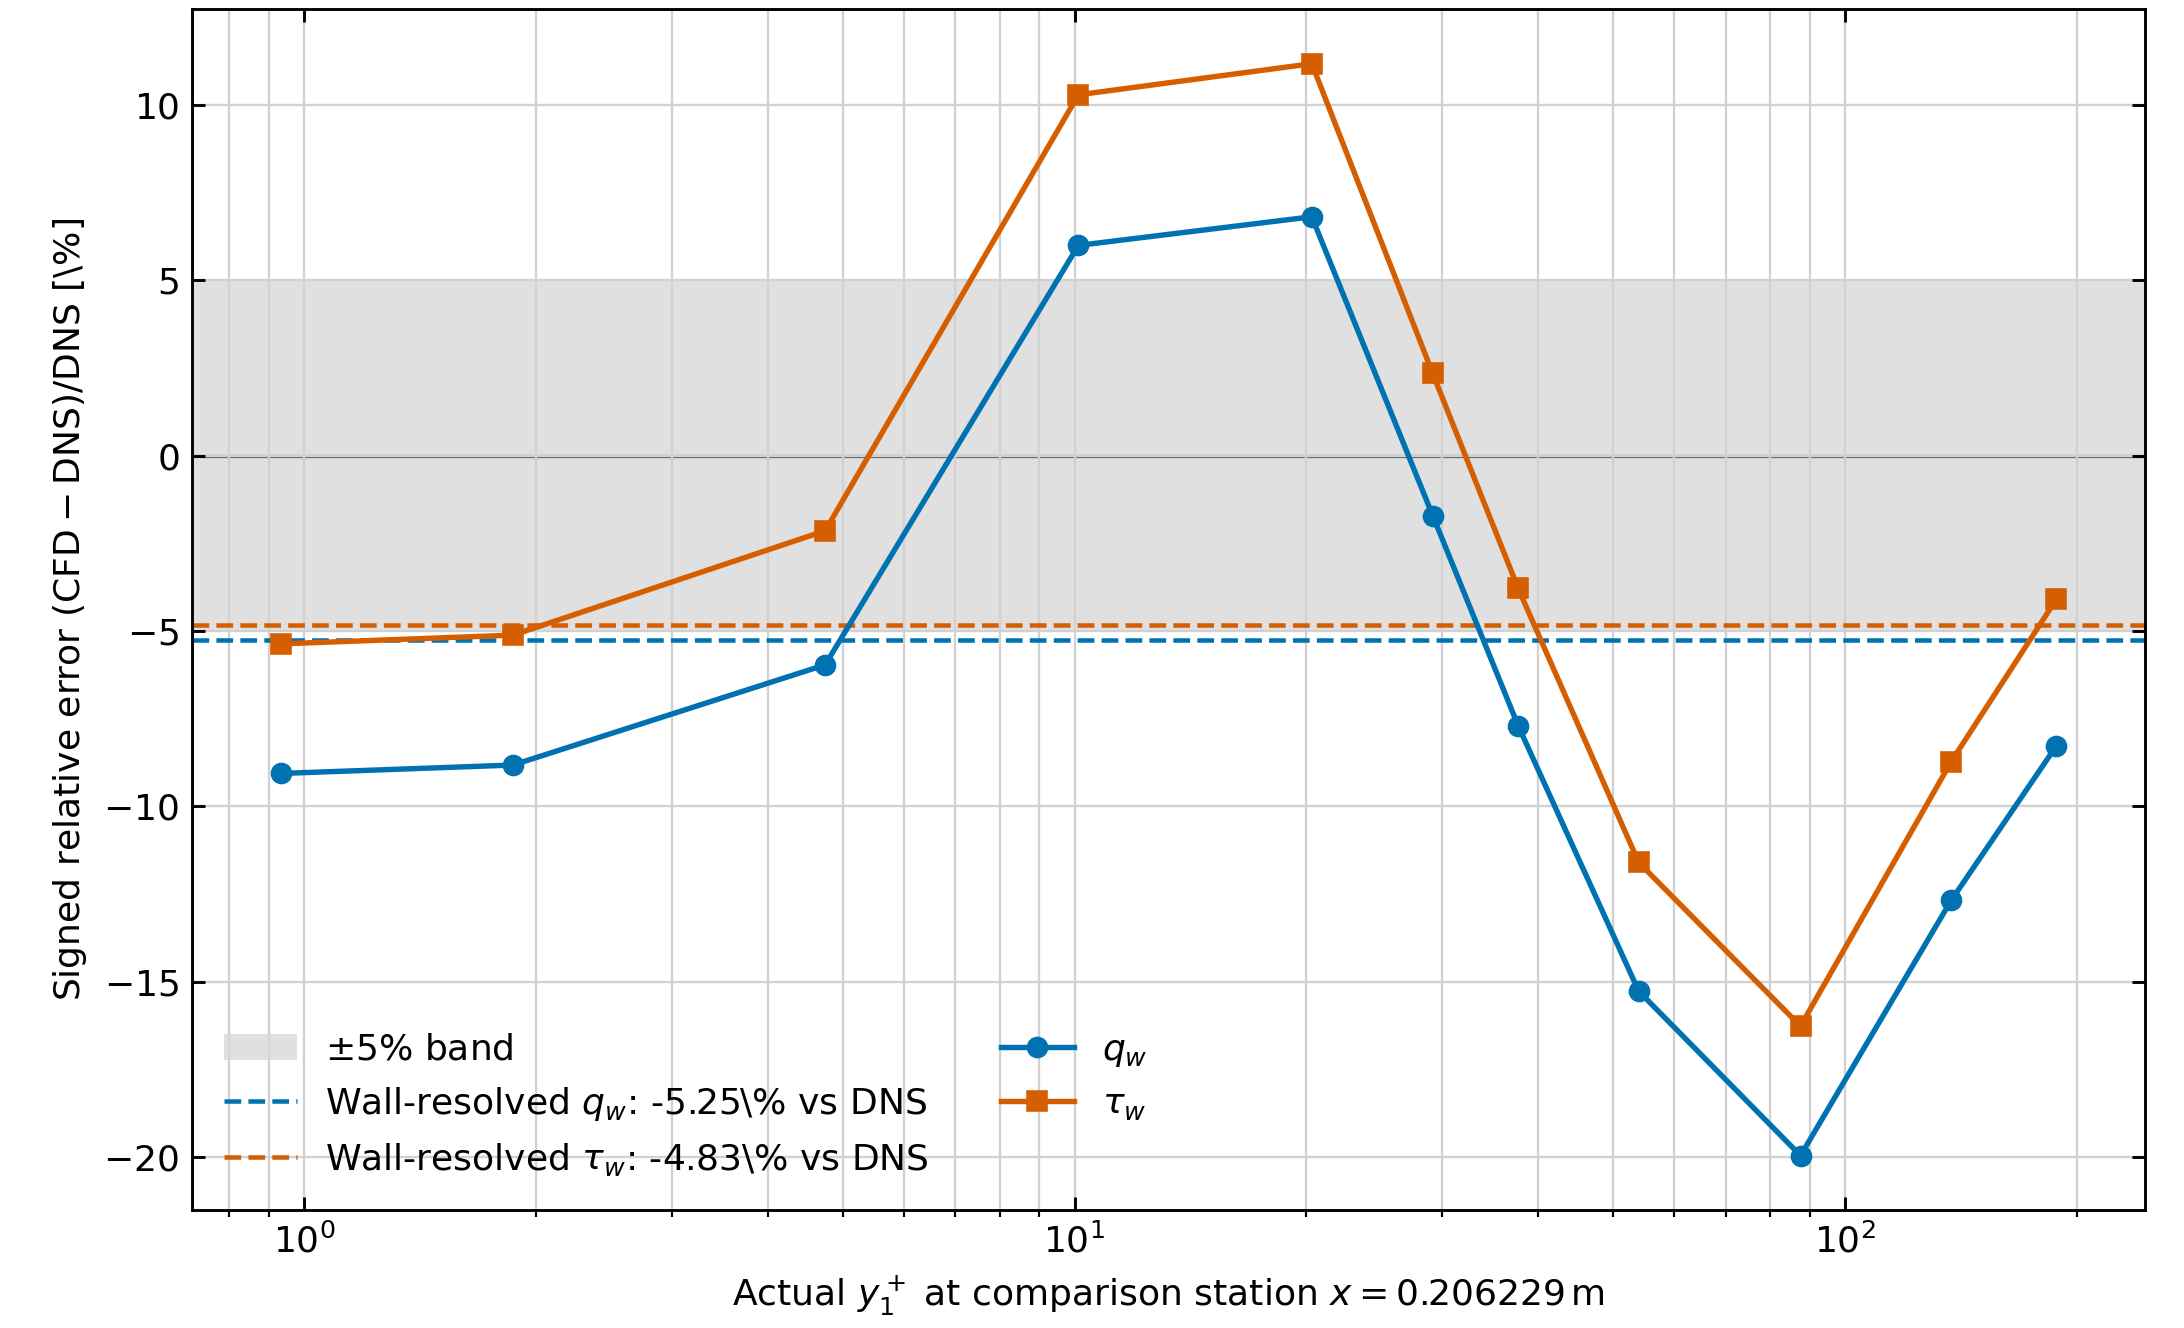
\includegraphics[width=\linewidth,height=.62\textheight,keepaspectratio]{07_Error_Isolation_Results/Figures/WallFunctions/04_ConvMesh_Griffin_M6Tw025.png}
    \caption{Griffin wall-function CFD with SA on conventional meshes for M6Tw025, using the DNS normalization and station of Figure~\ref{fig:WF:Li-M6Tw025_conventional_mesh}. Dashed lines denote the wall-resolved baseline; shading marks $\pm5\%$ relative to DNS.}
    \label{fig:WF:Griffin-M6Tw025_conventional_mesh}
\end{figure}

\subsection{Internal-face errors and a wall-normal spacing criterion}
\label{subsec:comparative:zpg:mesh-criterion}

For the FVM CFD, the numerical framework, is described in Section~\ref{sec:numerical-framework:discretization} and
distinguishes convective reconstruction from viscous flux evaluation. The direct wall-flux delivery of the wall-functions, as described in Section~\ref{subsec:wall-functions:direct-flux-delivery}, replaces the gradient-based evaluation at the wall, but gradients and transport coefficients at internal faces must still be approximated from the cell-centre values. For a predominantly streamwise boundary layer flow, neglecting $\partial V/\partial x$ relative to $\partial U/\partial y$ gives
\begin{equation}
    \tau_{xy}\simeq\mu_{\mathrm{eff}}\frac{\partial U}{\partial y},
    \qquad
    q_y=-\kappa_{\mathrm{eff}}\frac{\partial T}{\partial y}.
    \label{eq:erriso:diffusive-face-fluxes}
\end{equation}
Here $\tau_{xy}$ is the effective shear stress and $q_y$ is the effective heat-flux in the positive wall-normal direction. At internal faces parallel to the wall, these fluxes contribute to the discrete momentum and energy balances. As Equation~\ref{eq:erriso:diffusive-face-fluxes} shows, their evaluation relies both on wall-normal gradient approximations as well as interpolation of the effective viscosity $\mu_{\mathrm{eff}}$ and thermal conductivity $\kappa_{\mathrm{eff}}$ at the face location. Errors in either can therefore alter the flow field solution, which in turn feeds into the wall-function.
\par\medskip

Figure~\ref{fig:WF:exemplaray_y+10_mesh} visualizes the geometry of these operations on an exemplary conventional coarse wall-function mesh with a first-cell height of $y_1^+=10$ on the left and $y_1^+=30$ on the right. For equal adjacent cell thicknesses, the first centre at $y_1^+=10$ and the next at $y_2^+=30$ surround the internal face at $y_f^+=20$. The full centre separation, which the gradient approximation and coefficient interpolation needs to gap, is thus $h^+=20$. Increasing the first-cell height to $y_1^+=30$ also increases the stencil separation to $y_f^+=h^+=60$. Thus conventional coarsening changes both the wall-function sampling height and the distance over which internal-face transport is evaluated. The former already isolately evaluated in Section~\ref{sec:comparative:zpg:cross-comparison} and the latter is evaluated in this section.

\begin{figure}[H]
    \centering
    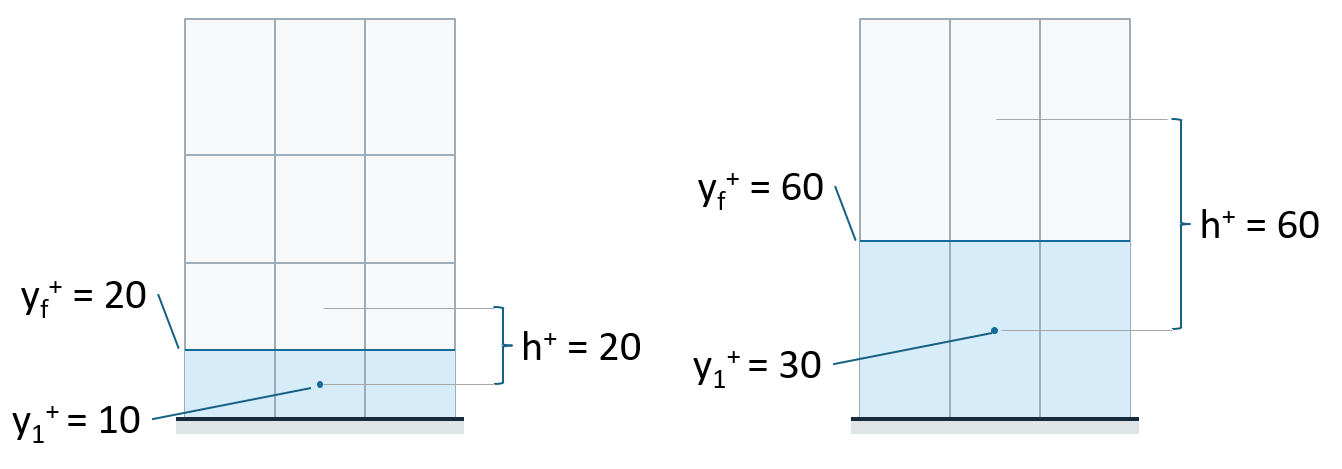
\includegraphics[width=\linewidth,height=.62\textheight,keepaspectratio]{07_Error_Isolation_Results/Figures/Recon/illustration_conv_coarse_mesh.png}
    \caption{Illustrative conventional near-wall meshes. For equal cell thicknesses adjacent to the first internal face, $y_1^+=10$ gives $y_f^+=h^+=20$ (left), while $y_1^+=30$ gives $y_f^+=h^+=60$ (right). Here $h^+$ is the full centre separation. The lower cell extends from the wall to the face, establishing an upper geometric link between the centre spacing $h^+$ and cell height of $h^+=y_f^+$.}
    \label{fig:WF:exemplaray_y+10_mesh}
\end{figure}

Figure~\ref{fig:WF:exemplaray_y+10_reconstruction_error} uses the M6Tw025 DNS temperature profile to illustrate a potential limitation of second-order accurate internal-face gradient reconstruction in a hypersonic cold-wall boundary layer. For the symmetric two-centre stencil considered here, the second-order accurate face-gradient approximation is the slope of a linear secant through the neighbouring cell-centre values. In this example, the secant connects the temperatures at $y^+=10$ and $30$, while the required gradient is the tangent slope at $y_f^+=20$. The pronounced cold-wall temperature peak causes substantial variation in curvature across this coarse stencil, and the two slopes differ visibly. Thus even a symmetric, second-order accurate approximation can poorly represent the local thermal gradient. This example illustrates the mechanism, while the spacing analysis below quantifies it over the profile. Here second-order accuracy refers to the leading error scaling with the square of the centre separation, not to a quadratic interpolating curve.

\begin{figure}[H]
    \centering
    % Figure provenance (WSL; absolute paths):
    %   Figure: /mnt/c/Users/MichaelGnadlinger/.codex/visualizations/2026/09/28/01a0e8e6-c3e6-7e32-a912-308b04eb3ffd/M6Tw025_temperature_profile_clean_600.png
    %   Python script:
    %     /mnt/c/Users/MichaelGnadlinger/.codex/visualizations/2026/09/28/01a0e8e6-c3e6-7e32-a912-308b04eb3ffd/plot_temperature_profile_clean_600.py
    %   Data / simulation roots (high-level):
    %     /home/mgnadlinger/Xue_et_al/flat_plate/M6Tw025/opt_mesh/reference
    %     /home/mgnadlinger/Xue_et_al/flat_plate/M6Tw025/Digitizations
    %   Note: Thesis image is resized and cropped to remove the title.
    % End figure provenance.
    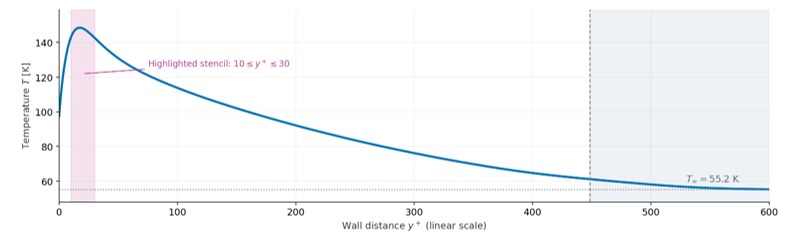
\includegraphics[width=\linewidth,height=.30\textheight,keepaspectratio]{07_Error_Isolation_Results/Figures/Recon/example_M6Tw025_Temperature_profile.png}
    \par\medskip
    % Figure provenance (WSL; absolute paths):
    %   Figure: /mnt/c/Users/MichaelGnadlinger/.codex/visualizations/2026/09/10/01a08aab-7a88-7450-b58c-b4f35bd01e8a/M6Tw025_temperature_full_and_y20.png
    %   Python script:
    %     /mnt/c/Users/MichaelGnadlinger/.codex/visualizations/2026/09/10/01a08aab-7a88-7450-b58c-b4f35bd01e8a/plot_temperature_y20.py
    %   Data / simulation roots (high-level):
    %     /home/mgnadlinger/Xue_et_al/flat_plate/M6Tw025/opt_mesh/reference
    %     /home/mgnadlinger/Xue_et_al/flat_plate/M6Tw025/Digitizations
    %   Note: Thesis image is a resized crop of panel (b), Temperature near the maximum.
    % End figure provenance.
    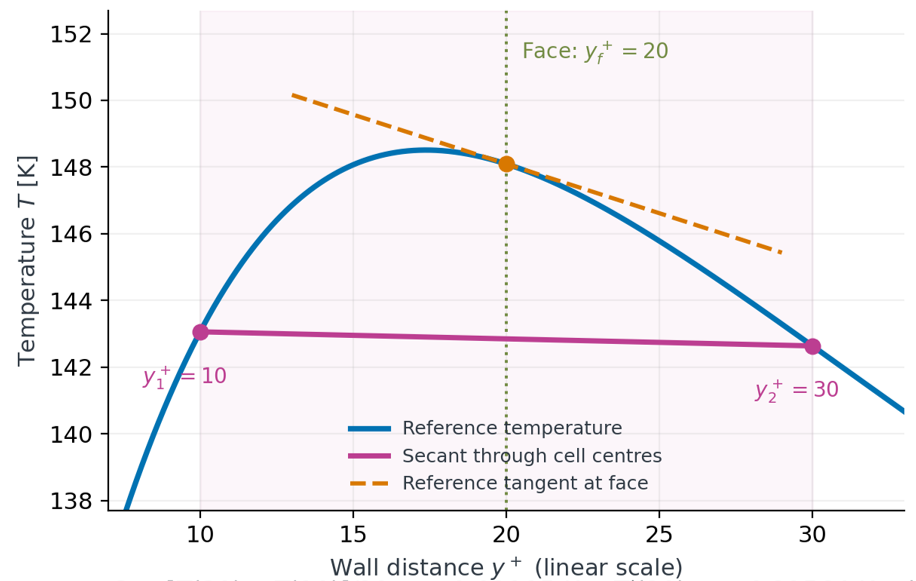
\includegraphics[width=\linewidth,height=.30\textheight,keepaspectratio]{07_Error_Isolation_Results/Figures/Recon/example_M6Tw025_Temperature_zoomed.png}
    \caption{M6Tw025 DNS temperature profile (top) and detail near its maximum (bottom). For the illustrative stencil in Figure~\ref{fig:WF:exemplaray_y+10_mesh}, the purple secant between $y^+=10$ and $30$ differs from the local tangent at the internal face $y_f^+=20$ (orange dashed line). The slopes illustrate the gradient contribution to thermal-diffusion error; the corresponding face flux also depends on the interpolated effective conductivity.}
    \label{fig:WF:exemplaray_y+10_reconstruction_error}
\end{figure}

The two-centre face-gradient approximation of a second-order accurate gradient reconstruction scheme is the slope of the linear secant through the neighbouring profile values:
\begin{equation}
    D_f\phi=\frac{\phi(y_R)-\phi(y_L)}{y_R-y_L}
    =\frac{\phi(y_f+b)-\phi(y_f-a)}{a+b},
    \qquad \phi\in\{T,U\},
\end{equation}
where $a=y_f-y_L$, $b=y_R-y_f$ and $h=a+b$. Unequal spacing introduces a truncation-error contribution $(b-a)\phi''(y_f)/2$. For the symmetric stencil, $a=b=h/2$, however this contribution vanishes and the secant slope approximates the face gradient with second-order accuracy. Taylor expansion expresses the secant slope as the exact tangent slope plus its error:
\begin{equation}
    \frac{\phi(y_f+h/2)-\phi(y_f-h/2)}{h}
    =\phi'(y_f)+\frac{h^2}{24}\phi'''(y_f)+O(h^4),
    \qquad \phi\in\{T,U\}.
    \label{eq:erriso:symmetric-gradient}
\end{equation}
For this symmetric stencil, the leading gradient error therefore depends on the change in curvature, $\phi'''$, rather than curvature alone. Dividing its magnitude by $|\phi'(y_f)|$ and prescribing a relative accuracy of the face gradient $\epsilon$ gives the spacing estimation $h_{\mathrm{grad}}$ for the second order accurate gradient reconstruction on a symmetric stencil as
\begin{equation}
    h_{\mathrm{grad}}\simeq
    \sqrt{24\epsilon\left|\frac{\phi'}{\phi'''}\right|}.
    \label{eq:erriso:gradient-spacing}
\end{equation}
Similarly, for symmetric linear interpolation of a coefficient $\Gamma\in\{\mu_{\mathrm{eff}},\kappa_{\mathrm{eff}}\}$, the face value is approximated by the mean of the two cell-centre values. Its leading error is $h^2\Gamma''(y_f)/8$, giving
\begin{equation}
    h_{\mathrm{interp}}\simeq
    \sqrt{8\epsilon\left|\frac{\Gamma}{\Gamma''}\right|}.
    \label{eq:erriso:coefficient-spacing}
\end{equation}
Equations~\eqref{eq:erriso:symmetric-gradient}--\eqref{eq:erriso:coefficient-spacing} identify the profile derivatives controlling the two operations. The envelopes below evaluate the corresponding finite-stencil errors directly on cubic-interpolation reconstructions of the digital reference profiles. The resulting spacing limits are the maximum centre separation that satisfies a prescribed relative error $\epsilon$ for each operation. 
\par\medskip

Figure~\ref{fig:WF:M6Tw025-profiles} shows exemplary the four profiles of the M6Tw025 case passed through this spacing analysis. DNS supplies M6Tw025 temperature and velocity, the matched wall-resolved SA solution supplies effective viscosity and conductivity. The effective transport properties need to be taken from the wall-resolved SA reference because not published with the DNS profiles. For the subsequent LowH\_M3 mesh design, all profiles come from the wall-resolved SA reference, because of the lack of published high-quality digital DNS data. In the Figure~\ref{fig:WF:M6Tw025-profiles} profiles it is immediatly apparant that the thermal profile present significantly more change in curvature than the velocity profile because of the sharp temperature peak near the wall. As identified in Equation~\eqref{eq:erriso:coefficient-spacing}, the transport coefficients rely on the curvature of the repsetive profiles, rather than the change in curvature, which for the M6Tw025 case has three pronounced regions of high curvature, directly at the wall because of the zero gradient Neumann boundary conditions there, at \(y \approx 0.0025 \mathrm{m}\) and \(y \approx 0.005 \mathrm{m}\) (see Figure~\ref{fig:WF:M6Tw025-profiles} bottom plots). 

\begin{figure}[H]
    \centering
    % Figure provenance (WSL; absolute paths):
    %   Figure: /home/mgnadlinger/Xue_et_al/flat_plate/M6Tw025/opt_mesh/spacing_limits/M6Tw025_DNS_and_wall_resolved_profiles_physical_y_linear.png
    %   Python script:
    %     /home/mgnadlinger/Xue_et_al/flat_plate/M6Tw025/opt_mesh/scripts/plot_requested_profiles.py
    %   Data / simulation roots (high-level):
    %     /home/mgnadlinger/Xue_et_al/flat_plate/M6Tw025/opt_mesh/reference
    %     /home/mgnadlinger/Xue_et_al/flat_plate/M6Tw025/Digitizations
    %     /home/mgnadlinger/Xue_et_al/flat_plate/M6Tw025/Li_SA/SA_Prt0p9_baseline
    %   Note: DNS temperature/velocity and SA effective transport use the frozen reference package; the SA
    %     station is x = 0.206229 m at time 15000.
    % End figure provenance.
    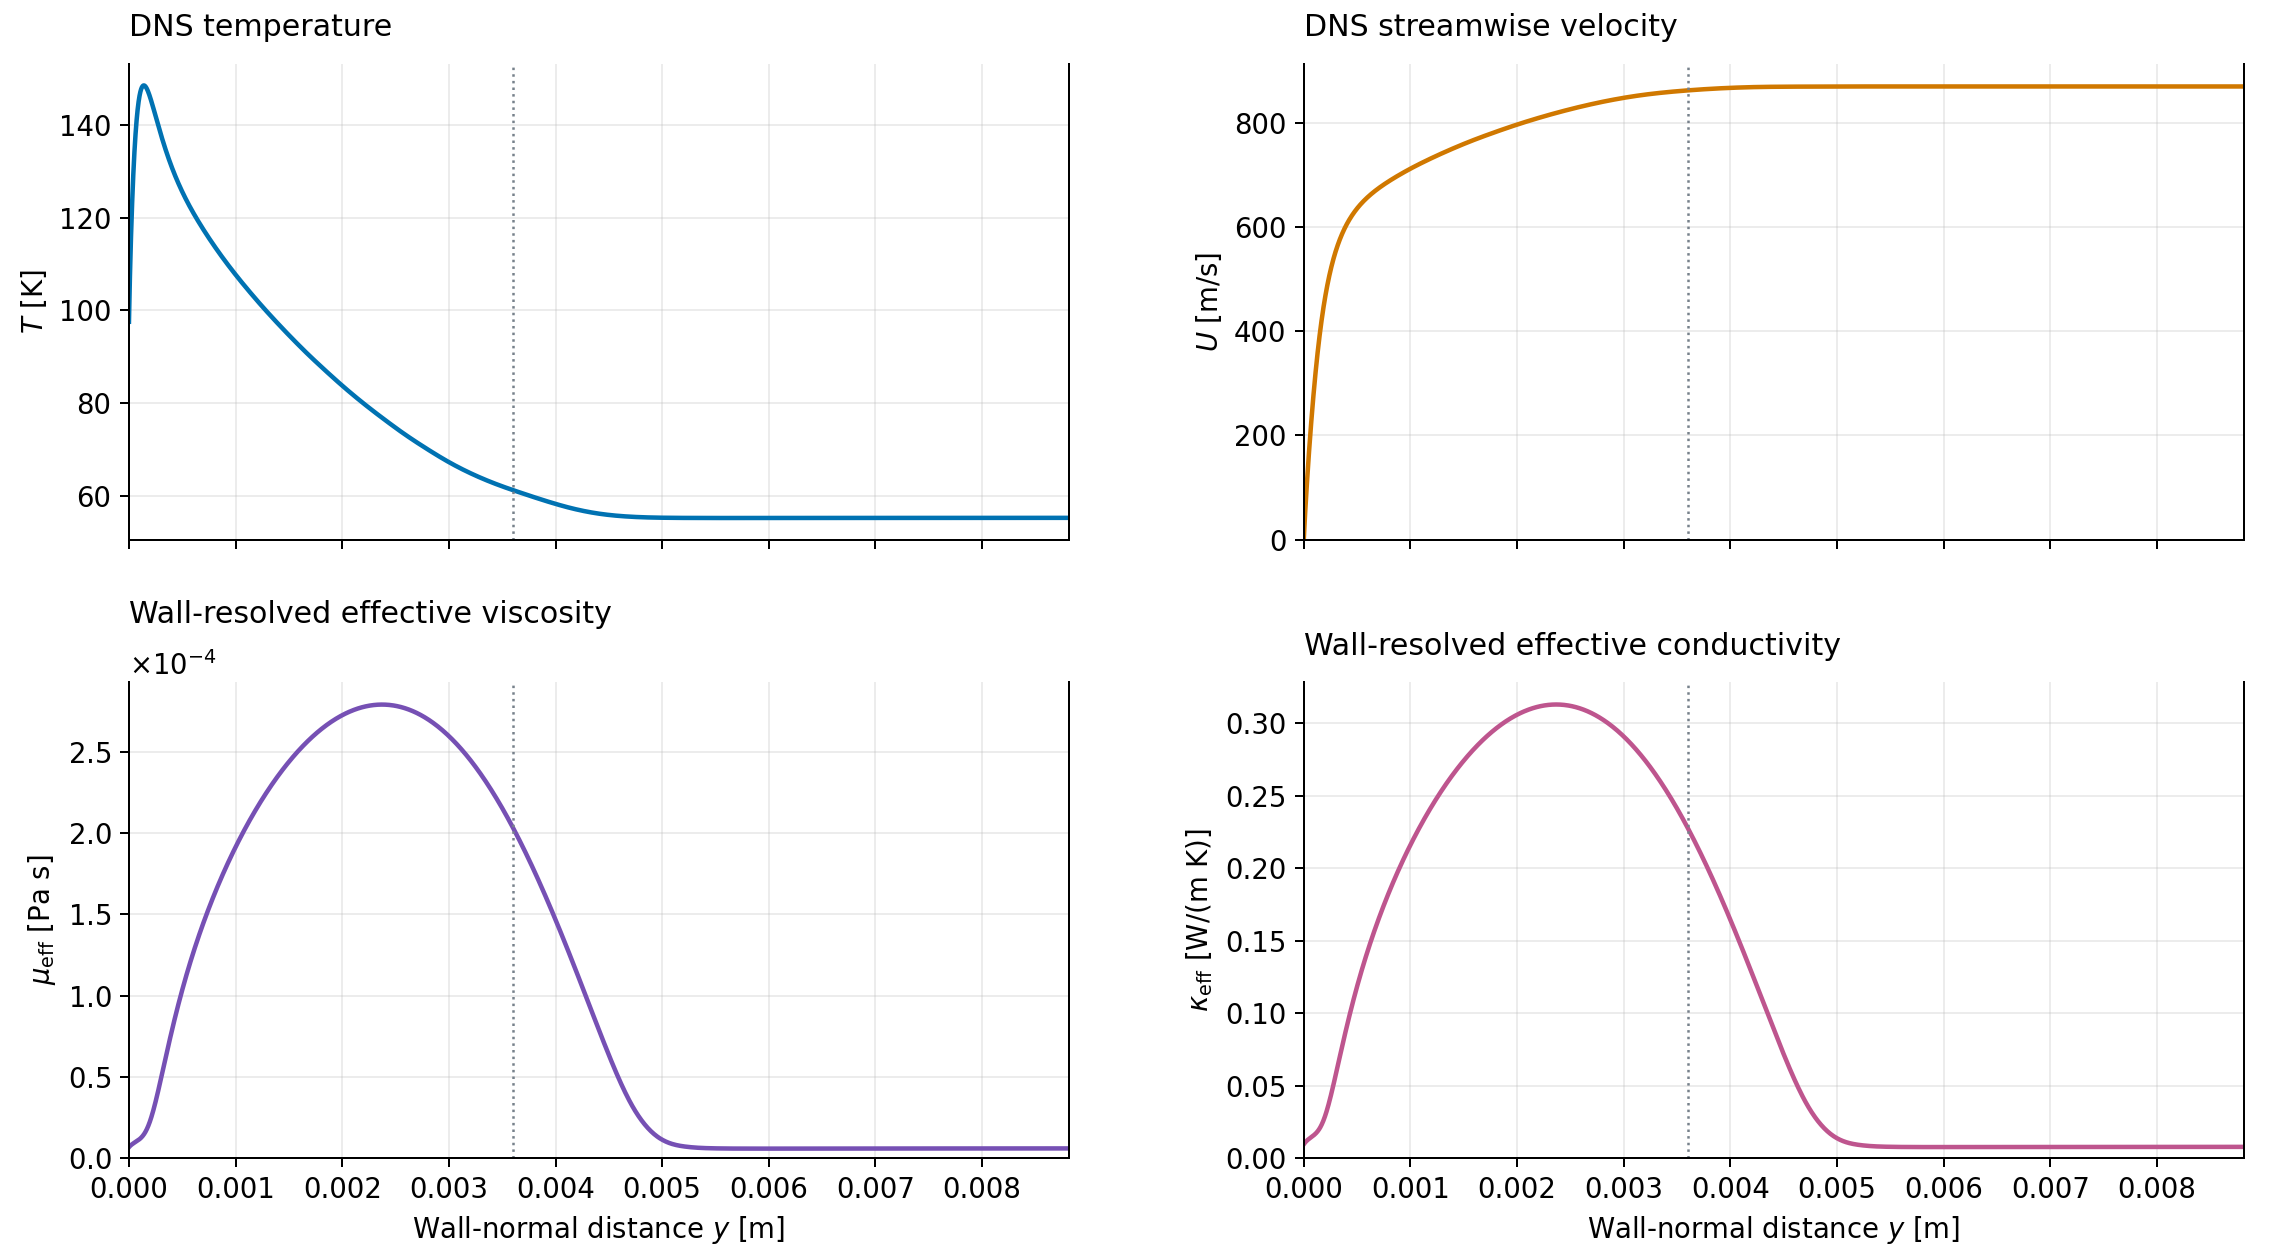
\includegraphics[width=\linewidth,height=.62\textheight,keepaspectratio]{07_Error_Isolation_Results/Figures/Recon/M6Tw025_DNS_BL_profiles_lin-y.png}
    \caption{Profiles underlying the M6Tw025 spacing assessment, plotted against physical wall-normal distance. DNS temperature and velocity are shown above; effective viscosity and thermal conductivity from the matched wall-resolved SA solution are shown below. The temperature maximum and the variation of effective transport motivate separate gradient and coefficient-interpolation criteria.}
    \label{fig:WF:M6Tw025-profiles}
\end{figure}

Using the found Equations \eqref{eq:erriso:gradient-spacing} and \eqref{eq:erriso:coefficient-spacing} that link the cell-centre spacing to the respective gradient reconstruction and interpolation errors, the M6Tw025 profiles of Figure~\ref{fig:WF:M6Tw025-profiles} are analysed. This results in the four individual spacing limits as shown in Figure~\ref{fig:WF:M6Tw025-3pct-envelope-all-quantities}. The resulting envelopes show, the allowable cell spacing $h$, for a given cell face position $y^+_f$ so that the relative errors for the gradient reconstruction or interpolation stay below a given tolerance of e.g. $\epsilon_{max}=3\%$.
\par\medskip

The cell spacing must also adhere to the upper geometric limit of $h^+\leq y_f^+$. At this limit two equal hight cells around a given face have centres at $y_f^+/2$ and $3y_f^+/2$, thus resulting in the lower cell extending all the way from the face to the wall. Thus the full centre separation equals the face-to-wall distance. This is the conventional coarse wall-function mesh geometry illustrated above in Figure~\ref{fig:WF:exemplaray_y+10_mesh}. A limit below this line requires a smaller centre separation at the same face position. a limit reaching it permits that conventional stencil under the selected local criterion. The cap is an adopted mesh constraint, not an error estimate.
\par\medskip

Figure~\ref{fig:WF:M6Tw025-3pct-envelope-all-quantities} shows the individual limits for $\epsilon=0.03$. The temperature-gradient limit has a sharp minimum near the temperature maximum as expected and hypthesized above. The coefficient interpolation and velocity-gradient reconstruction somewhat restrict other parts of the inner layer. At the exact Temperature peak, $T'=0$ thus the relative gradient error of Equations \eqref{eq:erriso:gradient-spacing} appraoches a asymptote - for the M6Tw025 case this is at around $y^+_f\approx 18$, in-line with the plotted temperature profile in Figure~\ref{fig:WF:exemplaray_y+10_reconstruction_error}. The sharp minimum reflects this conditioning as good as the cubic-interpolation of the given profile allows.

\begin{figure}[H]
    \centering
    % Figure provenance (WSL; absolute paths):
    %   Figure: /home/mgnadlinger/Xue_et_al/flat_plate/M6Tw025/opt_mesh/spacing_limits/M6Tw025_finite_spacing_3pct_relative_no_diagnostic_note.png
    %   Python scripts:
    %     /home/mgnadlinger/Xue_et_al/flat_plate/M6Tw025/opt_mesh/scripts/plot_requested_profiles.py
    %     /home/mgnadlinger/Xue_et_al/flat_plate/M6Tw025/opt_mesh/scripts/plot_analysis.py
    %   Data / simulation roots (high-level):
    %     /home/mgnadlinger/Xue_et_al/flat_plate/M6Tw025/opt_mesh/spacing_limits
    %     /home/mgnadlinger/Xue_et_al/flat_plate/M6Tw025/opt_mesh/reference
    %     /home/mgnadlinger/Xue_et_al/flat_plate/M6Tw025/Digitizations
    %     /home/mgnadlinger/Xue_et_al/flat_plate/M6Tw025/Li_SA/SA_Prt0p9_baseline
    %   Note: plot_analysis.py generates the finite-stencil limit tables; plot_requested_profiles.py exports
    %     this cubic-only figure.
    % End figure provenance.
    %   Print-size typography: regenerated at 170 mm width with 10 pt text; exact source table
    %     retained in Figures/Recon/spacing_font_sources/ (script, data and provenance).
    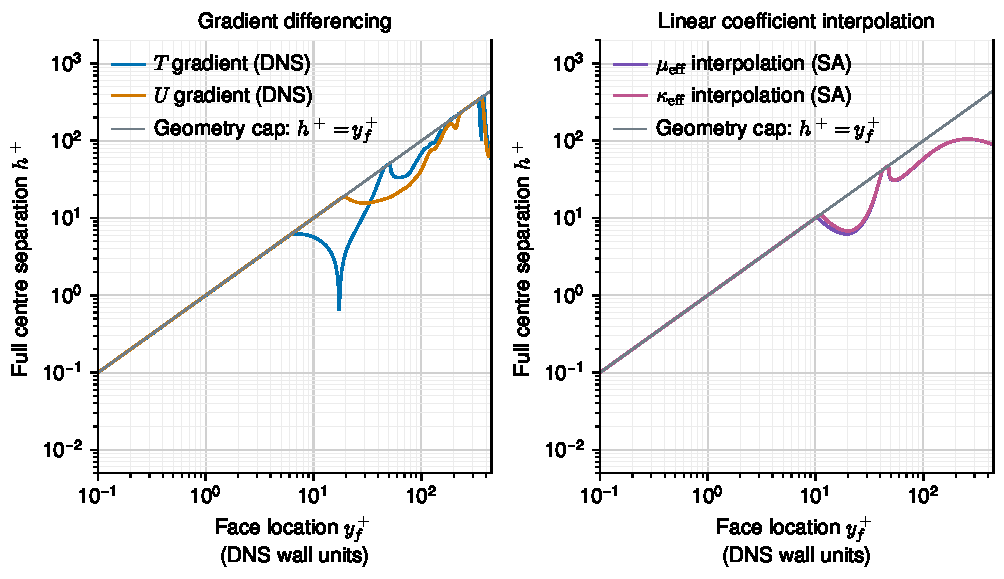
\includegraphics[width=\linewidth]{07_Error_Isolation_Results/Figures/Recon/M6Tw025_3pct_envelope.pdf}
    \caption{M6Tw025 spacing limits at a $3\%$ local component-error tolerance. The allowable full centre separation $h^+$ is plotted against internal-face position $y_f^+$ for centred differencing of DNS temperature and velocity (left) and linear interpolation of wall-resolved SA effective transport (right). Each limit is the first tolerance crossing evaluated on cubic profile reconstructions, capped by the adopted geometric condition $h^+\leq y_f^+$. Both coordinates use DNS wall units.}
    \label{fig:WF:M6Tw025-3pct-envelope-all-quantities}
\end{figure}

To satisfy all four component criteria of Figure~\ref{fig:WF:M6Tw025-3pct-envelope-all-quantities} simultaneously, the allowable spacing is their minimum at each face position, further limited by profile support and the geometric cap. Figure~\ref{fig:WF:M6Tw025-3pct-envelope-combined} is the resulting $3\%$ envelope. It converts the separate operator restrictions into a single wall-normal spacing requirement. Near the cold-wall temperature maximum, its large separation from $h^+=y_f^+$ quantifies why the conventional coarse stencil is inadequate and how much smaller the centre separation must be to avoid excessive errors. It must be emphasized that this is a local operator criterion, not a $3\%$ error bound on the wall heat-flux or shear stress. Additionally these four component errors can add constructively or destructively, so the combined envelope is not a direct error estimate, but it limits their individual contributions.

\begin{figure}[H]
    \centering
    % Figure provenance (WSL; absolute paths):
    %   Figure: /home/mgnadlinger/Xue_et_al/flat_plate/M6Tw025/opt_mesh/spacing_limits/M6Tw025_3pct_limits_only_font80.png
    %   Python scripts:
    %     /home/mgnadlinger/Xue_et_al/flat_plate/M6Tw025/opt_mesh/scripts/plot_cubic_limits_font80.py
    %     /home/mgnadlinger/Xue_et_al/flat_plate/M6Tw025/opt_mesh/scripts/plot_analysis.py
    %   Data / simulation roots (high-level):
    %     /home/mgnadlinger/Xue_et_al/flat_plate/M6Tw025/opt_mesh/spacing_limits
    %     /home/mgnadlinger/Xue_et_al/flat_plate/M6Tw025/opt_mesh/reference
    %     /home/mgnadlinger/Xue_et_al/flat_plate/M6Tw025/Digitizations
    %     /home/mgnadlinger/Xue_et_al/flat_plate/M6Tw025/Li_SA/SA_Prt0p9_baseline
    %   Note: Combined envelope is plotted from the finite-stencil limit tables generated by plot_analysis.py.
    % End figure provenance.
    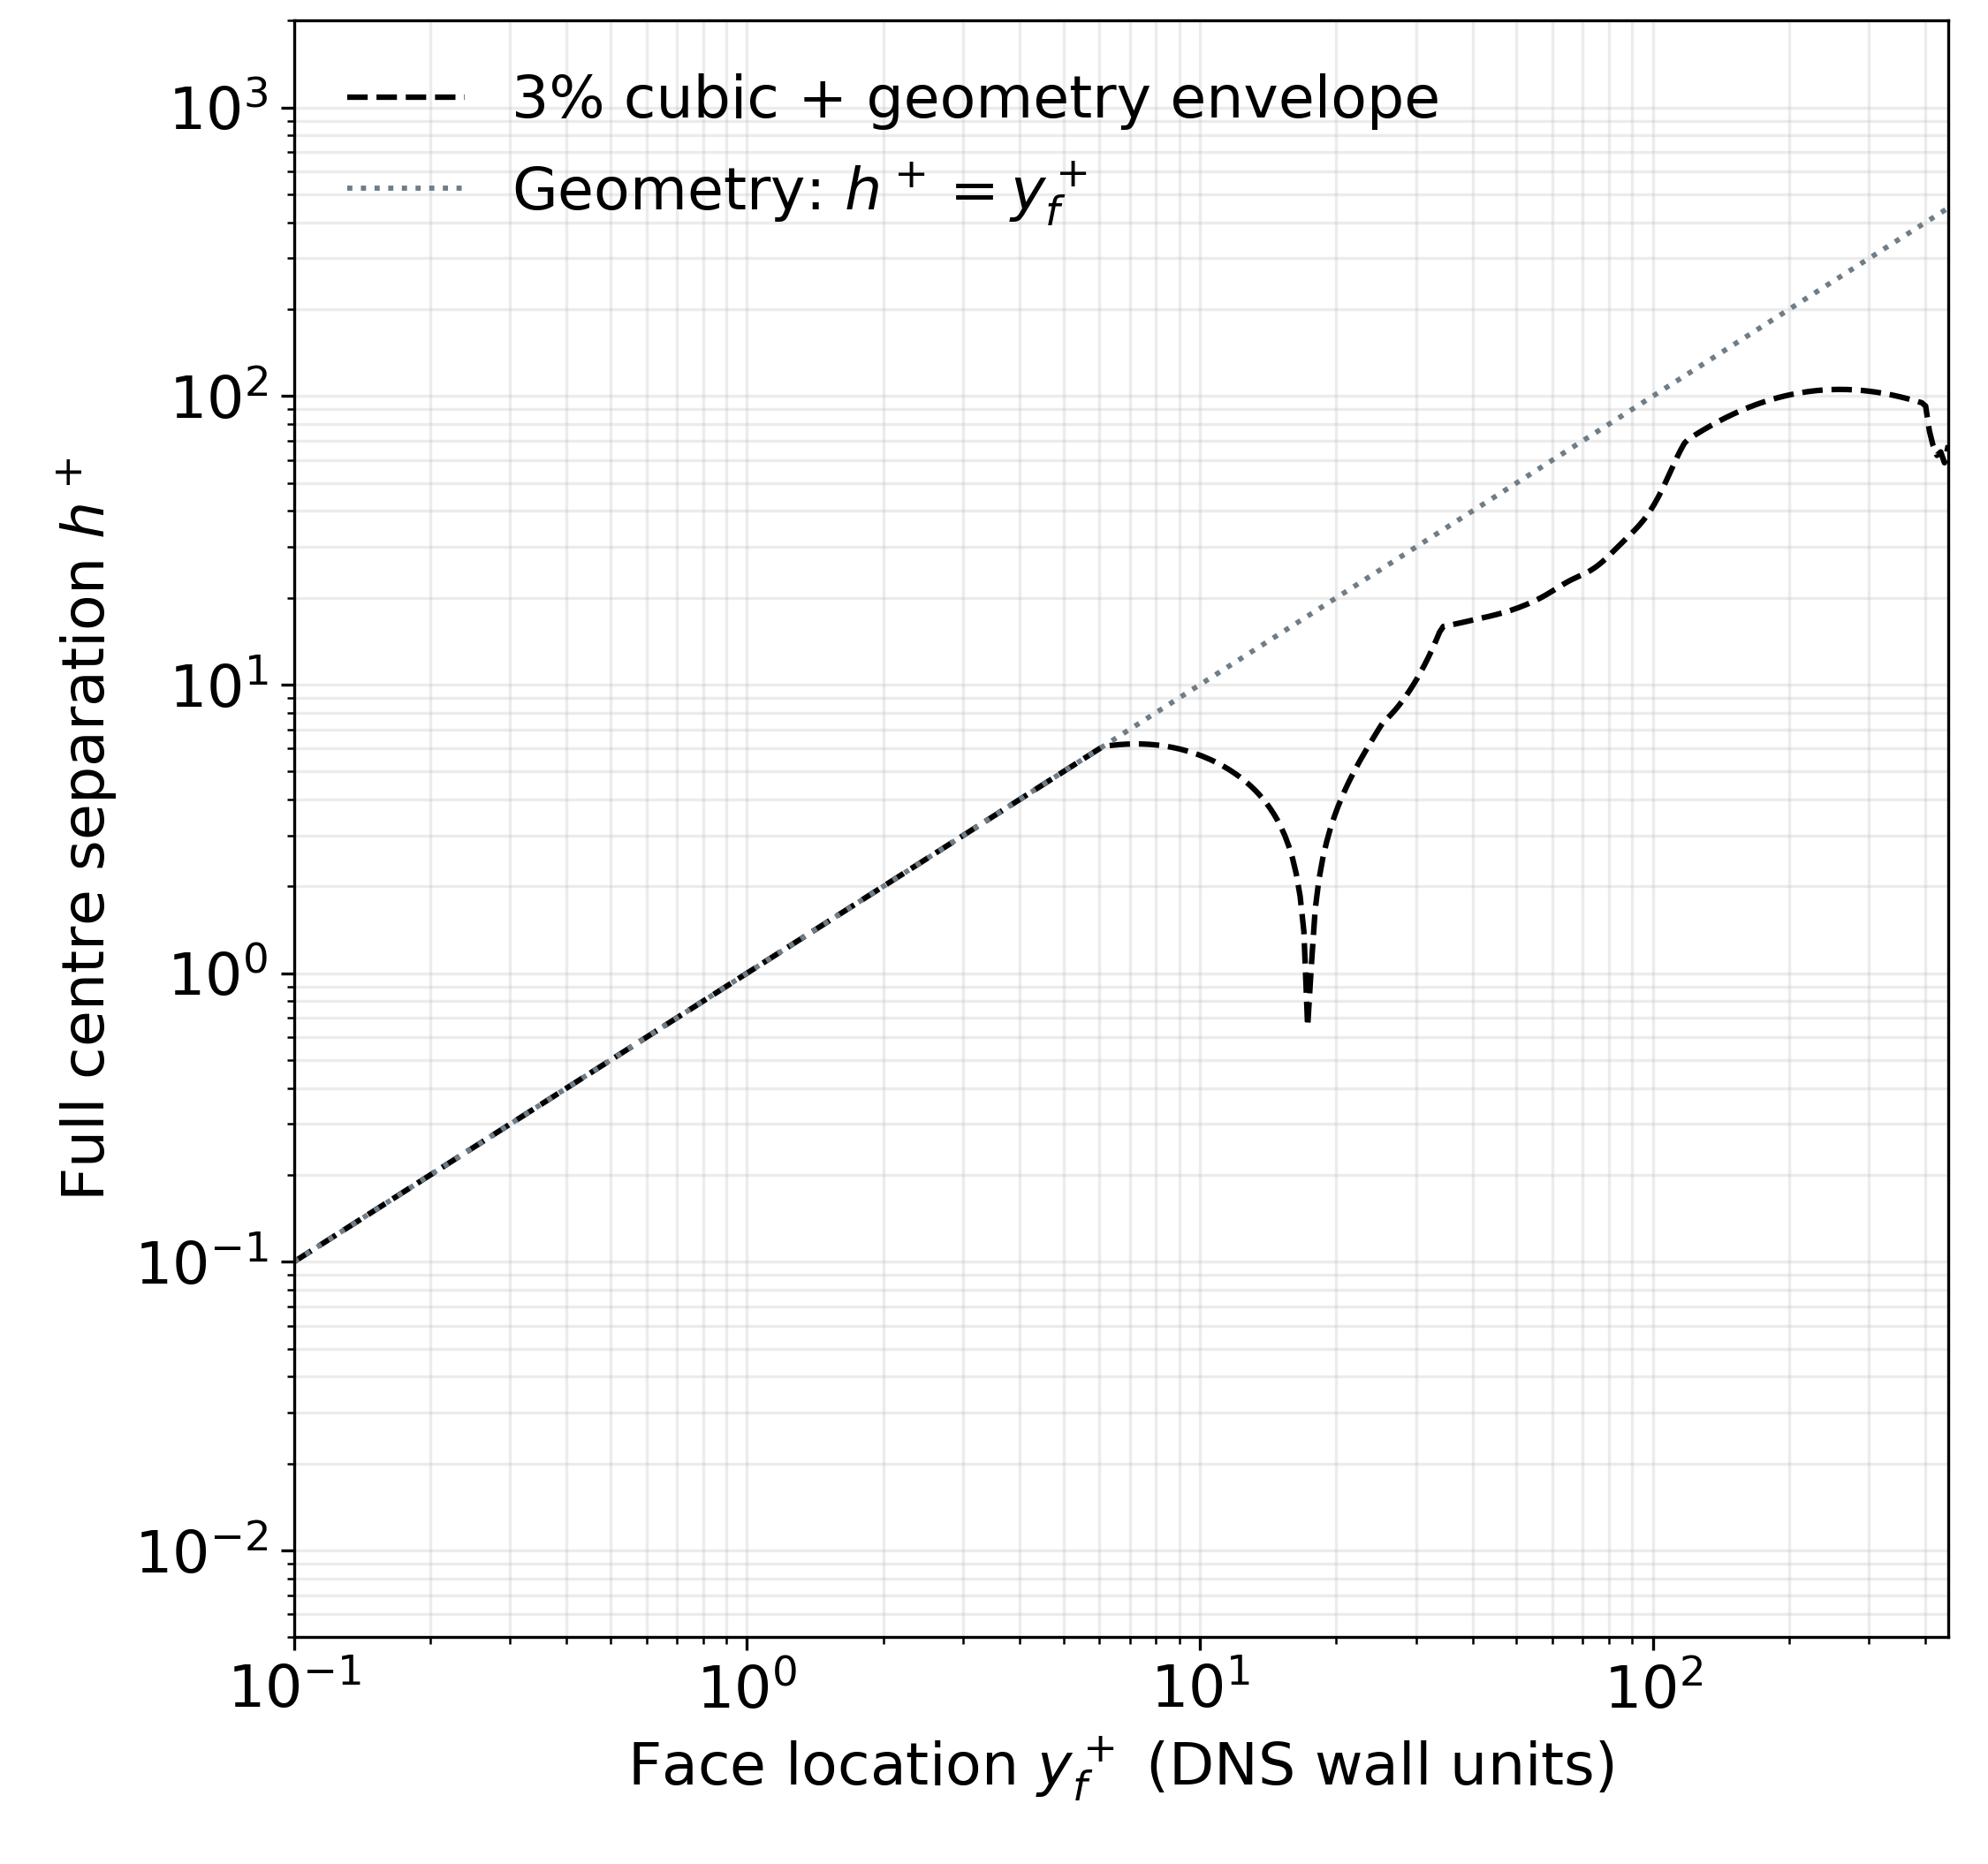
\includegraphics[width=0.7\linewidth,height=.62\textheight,keepaspectratio]{07_Error_Isolation_Results/Figures/WallFunctions/M6Tw025_3pct_envelope.png}
    \caption{Combined M6Tw025 spacing envelope for a $3\%$ component-error tolerance: the minimum of the four cubic-reference limits in Figure~\ref{fig:WF:M6Tw025-3pct-envelope-all-quantities}, profile support and the geometric cap $h^+=y_f^+$. The restrictive region near the temperature maximum requires substantially smaller centre separation than a conventional coarse stencil.}
    \label{fig:WF:M6Tw025-3pct-envelope-combined}
\end{figure}

Repeating the same analysis with $\epsilon=0.10$ gives Figure~\ref{fig:WF:M6Tw025-10pct-envelope-combined}. The restrictive minimum persists in the buffer region, whereas substantially larger spacings are admitted farther into the logarithmic region. Around $y_f^+\approx150$, the envelope reaches the geometric cap. Meaning a conventional symmetric coarse wall-function mesh stencil can locally satisfy the $10\%$ component tolerance and supports the finding discussed in Section~\ref{subsec:comparative:zpg:conventional-mesh}, that these log-layer regions are the ones used in the papers of Li et al. and Griffin et al. for validation purposes.

\begin{figure}[H]
    \centering
    % Figure provenance (WSL; absolute paths):
    %   Figure: /home/mgnadlinger/Xue_et_al/flat_plate/M6Tw025/opt_mesh/spacing_limits/M6Tw025_10pct_limits_only_font80.png
    %   Python scripts:
    %     /home/mgnadlinger/Xue_et_al/flat_plate/M6Tw025/opt_mesh/scripts/plot_cubic_limits_font80.py
    %     /home/mgnadlinger/Xue_et_al/flat_plate/M6Tw025/opt_mesh/scripts/plot_analysis.py
    %   Data / simulation roots (high-level):
    %     /home/mgnadlinger/Xue_et_al/flat_plate/M6Tw025/opt_mesh/spacing_limits
    %     /home/mgnadlinger/Xue_et_al/flat_plate/M6Tw025/opt_mesh/reference
    %     /home/mgnadlinger/Xue_et_al/flat_plate/M6Tw025/Digitizations
    %     /home/mgnadlinger/Xue_et_al/flat_plate/M6Tw025/Li_SA/SA_Prt0p9_baseline
    %   Note: Combined envelope is plotted from the finite-stencil limit tables generated by plot_analysis.py.
    % End figure provenance.
    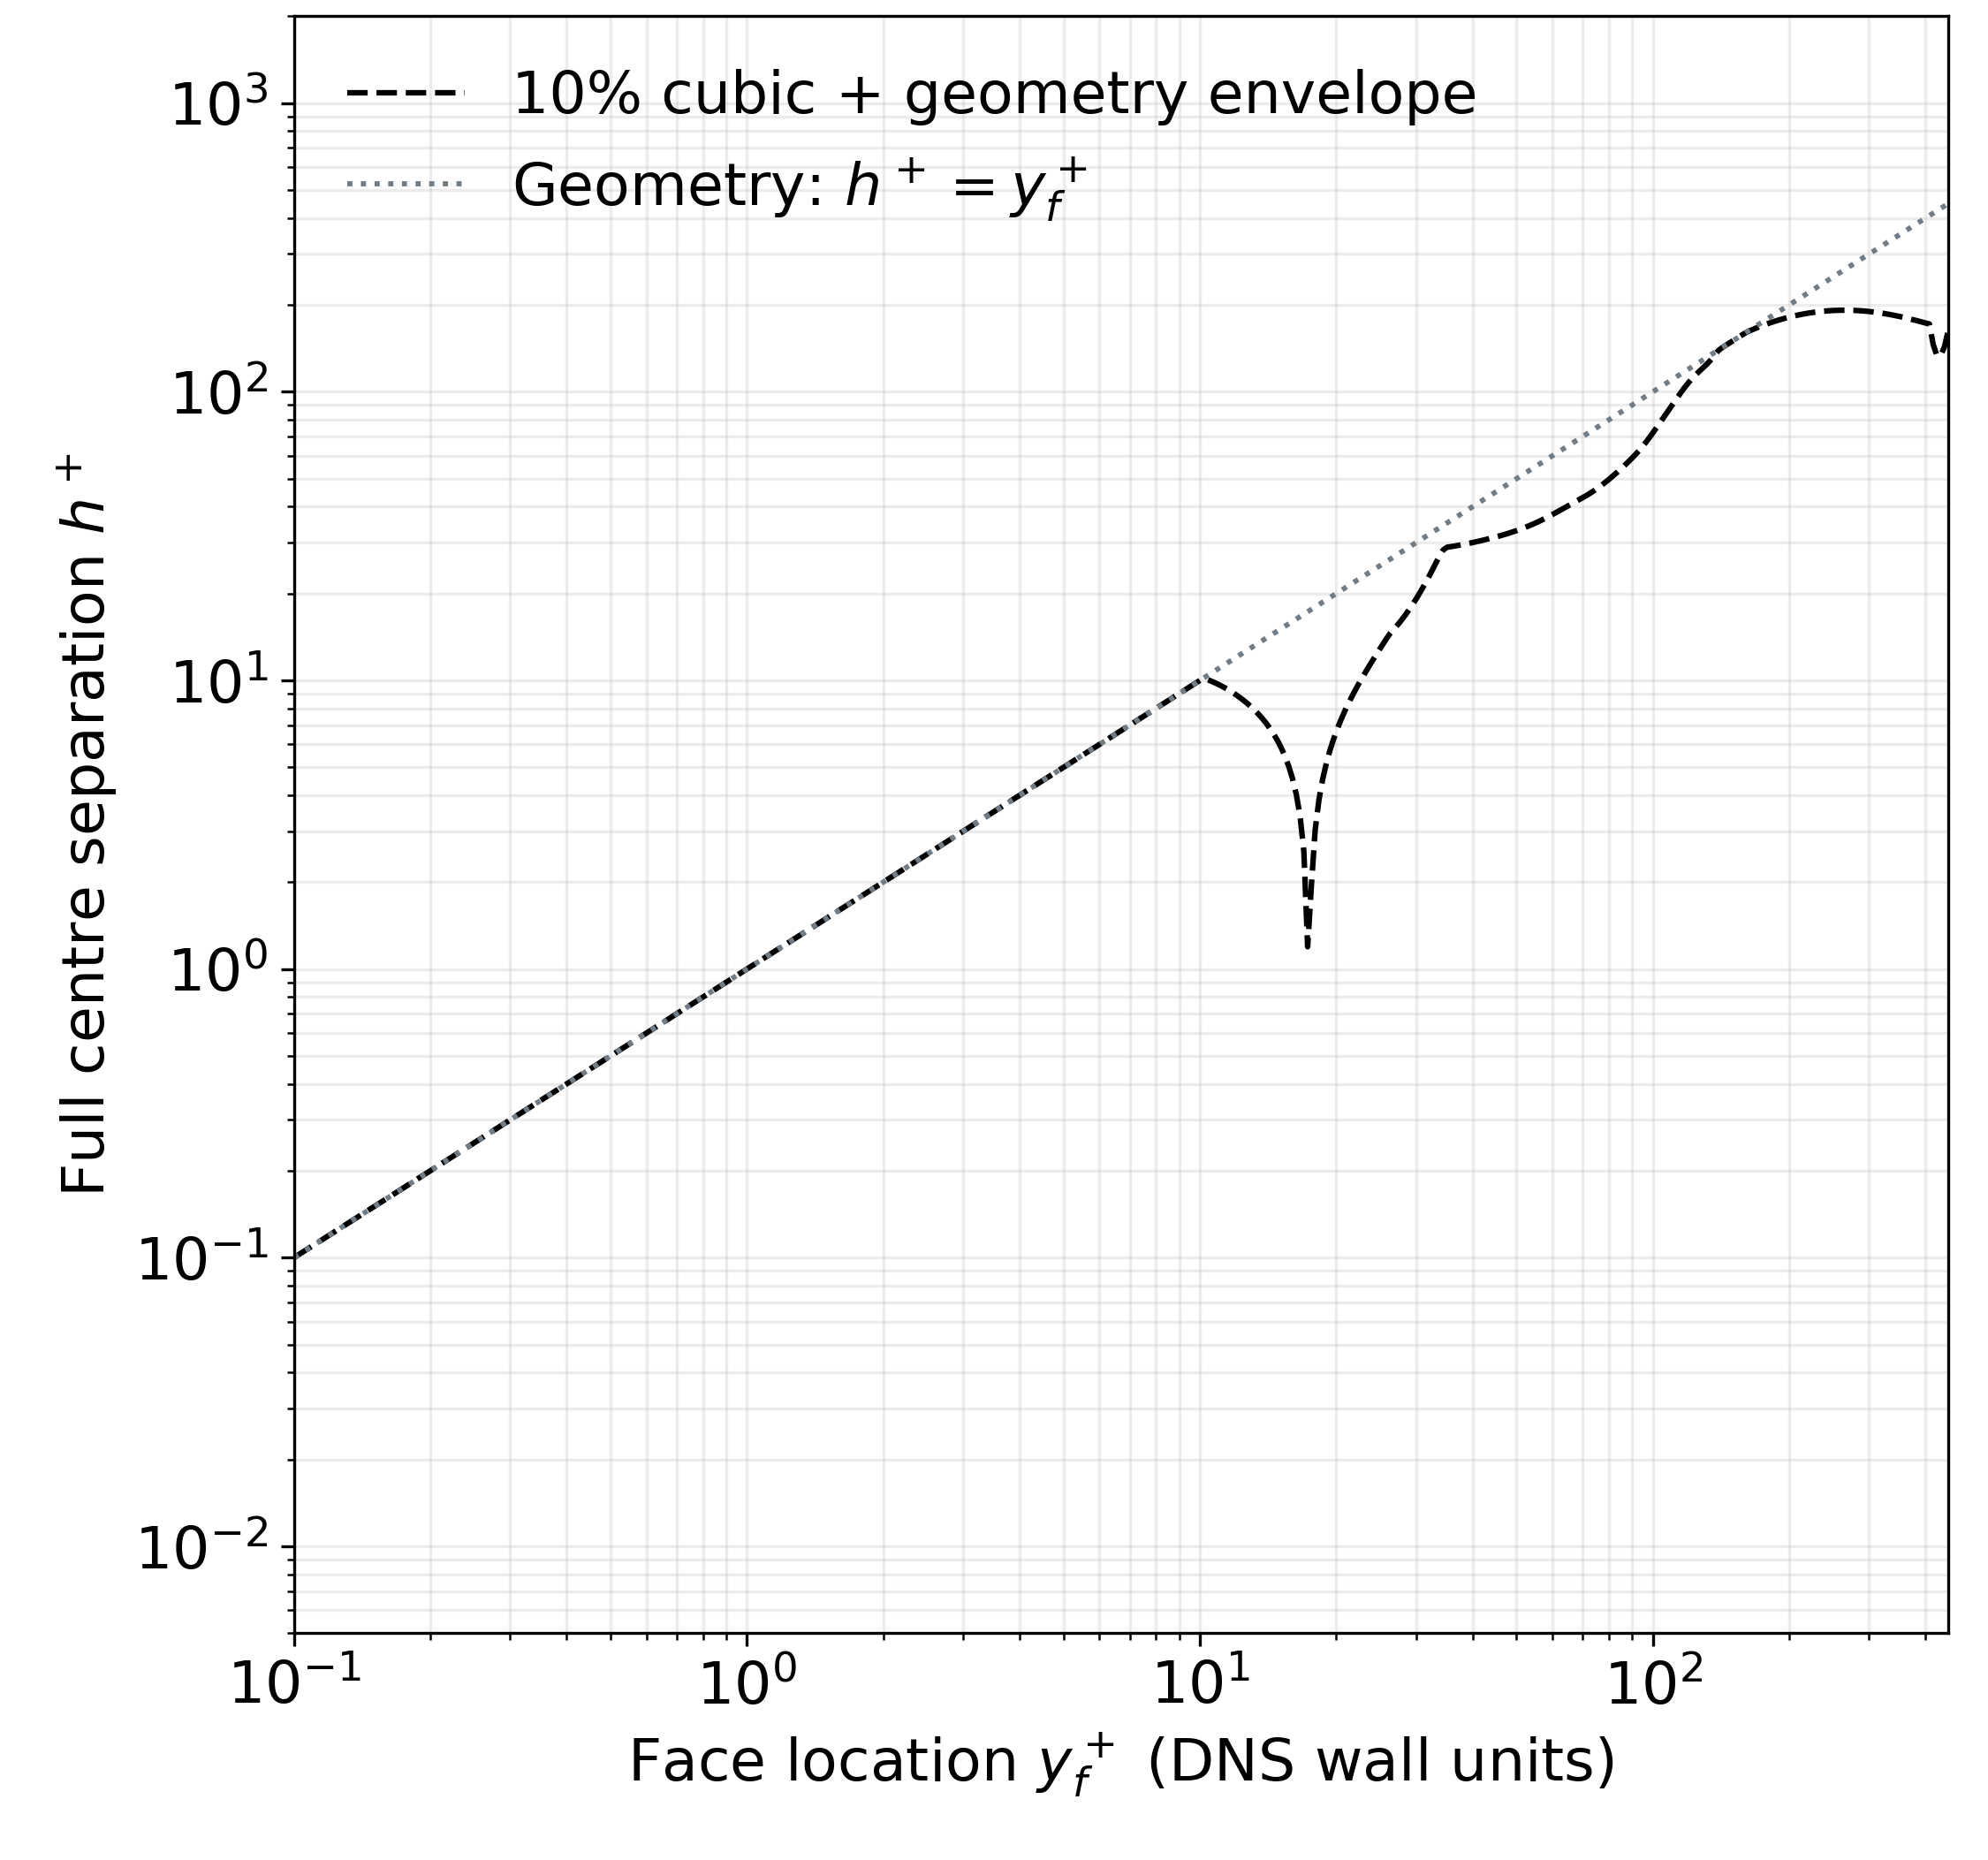
\includegraphics[width=0.7\linewidth,height=.62\textheight,keepaspectratio]{07_Error_Isolation_Results/Figures/WallFunctions/M6Tw025_10pct_envelope.png}
    \caption{Combined M6Tw025 spacing envelope with the local component-error tolerance relaxed to $10\%$. The restrictive minimum near the temperature maximum persists, while larger spacings are permitted farther outward. Around $y_f^+\approx150$, the envelope reaches the geometric cap and locally admits the conventional symmetric first-face stencil of Figure~\ref{fig:WF:exemplaray_y+10_mesh}. This is a local operator criterion, rather than a $10\%$ bound on CFD wall quantities.}
    \label{fig:WF:M6Tw025-10pct-envelope-combined}
\end{figure}

The physical reason on why this meshing restriction only arises now in hypersonic cold-wall boundary layers, and not in the subsonic or adiabatic-wall hypersonic cases can be seen in the comparative Figures~\ref{fig:WF:dns-velocity-profiles-linear} and~\ref{fig:WF:dns-temperature-profiles-linear}. There the M6Tw025 case is compared to the near-adiabatic M6Tw076 case and a transonic cold-wall case \textit{C09} of \cite{iwatani2025subharmonic}. Neither of the latter two cases show a pronounced temperature peak, and therefore the curvature variation is much less.

\begin{figure}[H]
    \centering
    % Figure provenance (paths relative to the thesis workspace root):
    % Original vector export: tmp/boundary_layer_profile_comparison/velocity_profiles_linear.pdf
    % Generating script: tmp/boundary_layer_profile_comparison/plot_linear_profiles.py
    % Shared data loading and styles: tmp/boundary_layer_profile_comparison/plot_profiles.py
    % Retained DNS files and preprocessing: tmp/boundary_layer_profile_comparison/raw/
    % Scaling checks and source URLs: tmp/boundary_layer_profile_comparison/source_notes.txt
    % Same DNS samples and normalizations as fig:background:dns-velocity-profiles:
    % Zhang, Duan and Choudhari (2018), DOI 10.2514/1.J057296;
    % Iwatani, Asada and Kawai (2025), DOI 10.1016/j.ijheatfluidflow.2025.109896.
    % C09: X=11, inferred velocity factor 0.8, conventional y+ reconstructed
    % from archived skin friction and wall properties, as documented in the background.
    % Linear y+ from 0 to 1200 includes all native samples and the wall points.
    % Copied without cropping or resizing the source PDF.
    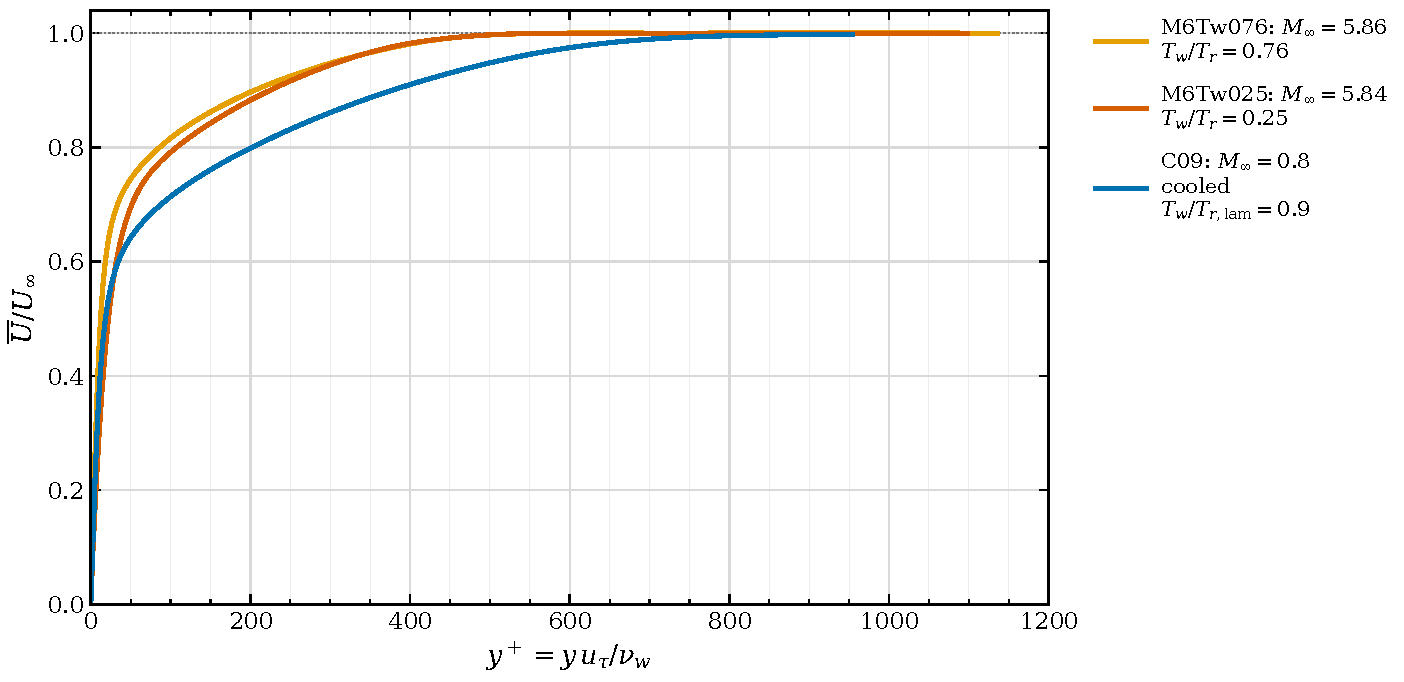
\includegraphics[width=\linewidth]{07_Error_Isolation_Results/Figures/Recon/velocity_profiles_linear.pdf}
    \caption[DNS velocity profiles on a linear wall-normal coordinate]{Freestream-normalized DNS velocity profiles for M6Tw076, M6Tw025 and C09, using the same data and normalization as Figure~\ref{fig:background:dns-velocity-profiles}, now plotted against linear \(y^+\). The native wall points at \(y^+=0\) are included.}
    \label{fig:WF:dns-velocity-profiles-linear}
\end{figure}

\begin{figure}[H]
    \centering
    % Figure provenance (paths relative to the thesis workspace root):
    % Original vector export: tmp/boundary_layer_profile_comparison/temperature_profiles_linear.pdf
    % Generating scripts, retained source data and scaling conventions:
    % as for fig:WF:dns-velocity-profiles-linear immediately above.
    % Native Reynolds-mean T/Tinf values are retained for all three cases.
    % Same thermal profiles as fig:background:dns-temperature-profiles;
    % linear y+ from 0 to 1200, including the native wall points, also in the C09 inset.
    % Copied without cropping or resizing the source PDF.
    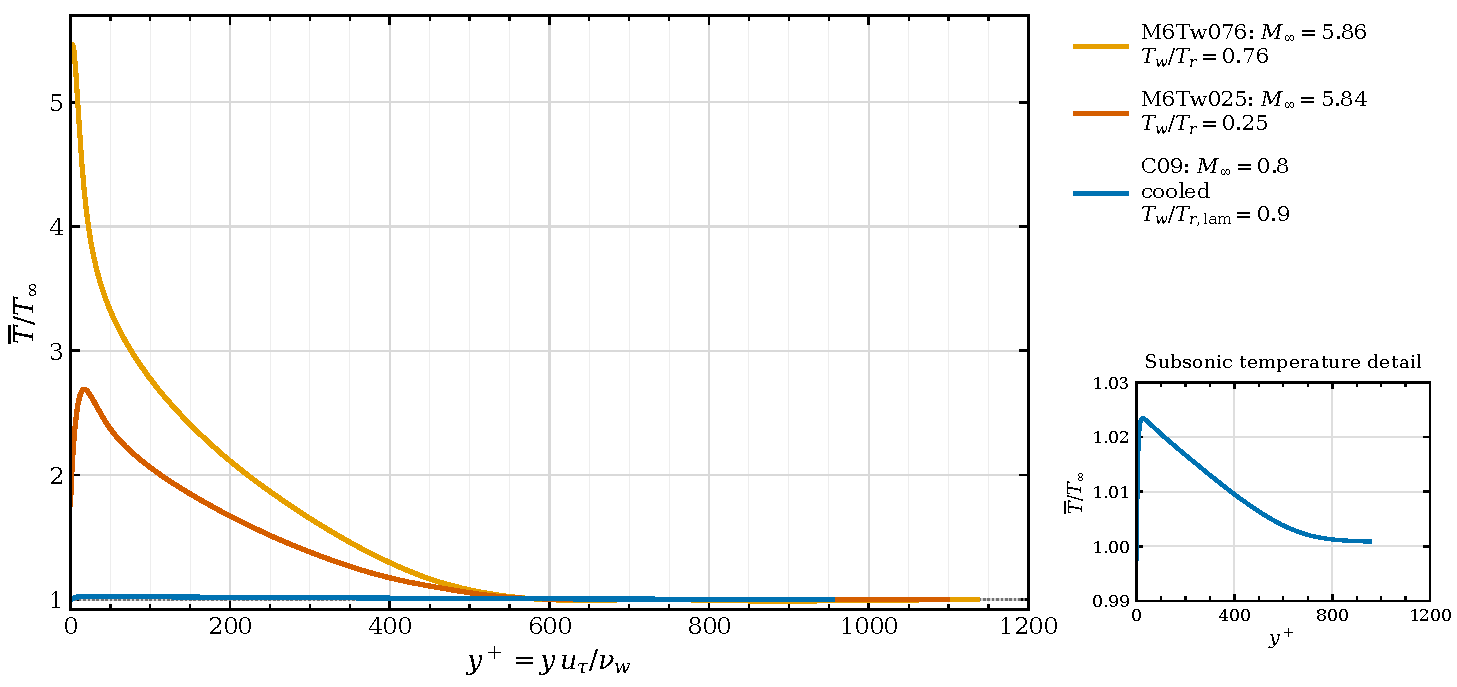
\includegraphics[width=\linewidth]{07_Error_Isolation_Results/Figures/Recon/temperature_profiles_linear.pdf}
    \caption[Linear thermal profiles and curvature variation near the cold-wall peak]{DNS temperature profiles from Figure~\ref{fig:background:dns-temperature-profiles}, shown on a linear \(y^+\) axis to better visualize the pronounced change in curvature associated with the hypersonic cold-wall M6Tw025 temperature peak. Since \(y^+\) is proportional to physical \(y\) within each case, this view connects the thermal-profile structure to finite stencil spacing and the reconstruction error illustrated by the secant--tangent comparison in Figure~\ref{fig:WF:exemplaray_y+10_reconstruction_error}. The C09 inset uses a separate vertical scale.}
    \label{fig:WF:dns-temperature-profiles-linear}
\end{figure}

All in all, the above analysis shows that the conventional coarse wall-function mesh stencil, paired with second-order accurate schemes, is not sufficient to resolve the internal-face transport in hypersonic cold-wall boundary layers. The pronounced temperature peak causes a large change in curvature, which in turn requires a much smaller centre separation than the conventional coarse wall-function mesh stencil provides. This novel mesh requirement is thus only dependant on the boundary layer profile and numerical schemes, in turn this requirement also applies to wall-resolved runs. In other words, the wall-functions can be understood as just a different heat-flux and shear stress relation than the convential linear correlation between the first off-wall cell cetner to the wall, as described for wall-resolved RANS in Equation~\eqref{eq:q_w_openFOAM_math}. But with the very low first-cell requirement of these wall-resolved runs on hypersonic cold-walls (i.e. the first-cell acoustic Reynolds number must be below 1 as discussed in Section~\ref{sec:evaluation:mesh-families-yplus}), only very extreme growth rates of the boundary layer mesh may run into any appreciable internal-face transport error, thus it remained undiscussed so far.
\par\medskip

The following section will show how proof this hypothesis by isolating these discretization errors through constructing boundary layer-informed meshes that satisfy the above discussed $3\%$ criterion.

\subsection{Wall functions on boundary layer-informed meshes}
\label{subsec:comparative:zpg:informed-mesh}

To test the above discussed error due to spatial discretization in CFD, families of boundary layer-informed meshes are constructed for prescribed wall-function sampling positions. This allows the wall-function sample to be swept over the whole $y^+$ range similar to the wall-closures a-priori analysis in Section~\ref{subsec:erriso:apriori-solver} and conventional mesh CFD runs in Figures~\ref{fig:WF:Li-LowHM3_conventional_mesh}--\ref{fig:WF:Griffin-M6Tw025_conventional_mesh}, while the internal-face spacing is controlled by the above discussed $3\%$ criterion. This arrangement reduces the coupling between moving the wall-function sample and the boundary layer spatial discretization.
\par\medskip

Figures~\ref{fig:WF:LowHM3-3pct-mesh-sweep} and~\ref{fig:WF:M6Tw025-3pct-mesh-sweep} show the resulting families for the M6Tw025 and LowH\_M3 case respectivly. The dotted and dashed lines are taken and constructed as described in the boundary layer analysis Section~\ref{subsec:comparative:zpg:mesh-criterion} above - specifically for the M6Two025 case, the Figure~\ref{fig:WF:M6Tw025-3pct-mesh-sweep} dashed and dotted lines are the same as in the Figure~\ref{fig:WF:M6Tw025-3pct-envelope-combined}. For the construction of the mesh families (see Figures~\ref{fig:WF:LowHM3-3pct-mesh-sweep} and~\ref{fig:WF:M6Tw025-3pct-mesh-sweep} right plots), a desired wall-function sampling height is prescribed and the internal-face spacing around it is then grown up until the allowable  discretization error of e.g. $3\%$ against the known profile is reached. This is continued until the whole boundary layer is covered. The resulting meshes are not a bound on the total CFD error or a proof of a globally optimal meshing, but aim to provide an isolation from this error source. The generated meshes are subsequently re-checked against the known boundary layer profiles, using their actual, generally unsymmetric, centre-to-face distances to ensure the desired spacing criterion is really satisfied.

\begin{figure}[H]
    \centering
    % Figure provenance (WSL; absolute paths):
    %   Figure: /home/mgnadlinger/WF_validation/LowH_M3/opt_meshes/marching_design/LowH_M3_mesh_sweep_3pct.png
    %   Python script:
    %     /home/mgnadlinger/WF_validation/LowH_M3/opt_meshes/marching_design/plot_mesh_report.py
    %   Data / simulation roots (high-level):
    %     /home/mgnadlinger/WF_validation/LowH_M3/opt_meshes/marching_design/3pct
    %     /home/mgnadlinger/WF_validation/LowH_M3/opt_meshes/marching_design/reference
    %     /home/mgnadlinger/WF_validation/LowH_M3/opt_meshes/Li_fitted_3pct_minCells_SA
    %     /home/mgnadlinger/WF_validation/LowH_M3/wall_resolved/SA/LowH_M3
    %   Note: Mesh-design report uses the frozen wall-resolved SA reference and the written fitted-Li mesh
    %     family.
    % End figure provenance.
    %   Print-size typography: regenerated at 170 mm width with 10 pt text; exact source data
    %     and local plotting script retained in Figures/WallFunctions/mesh_sweep_font_sources/.
    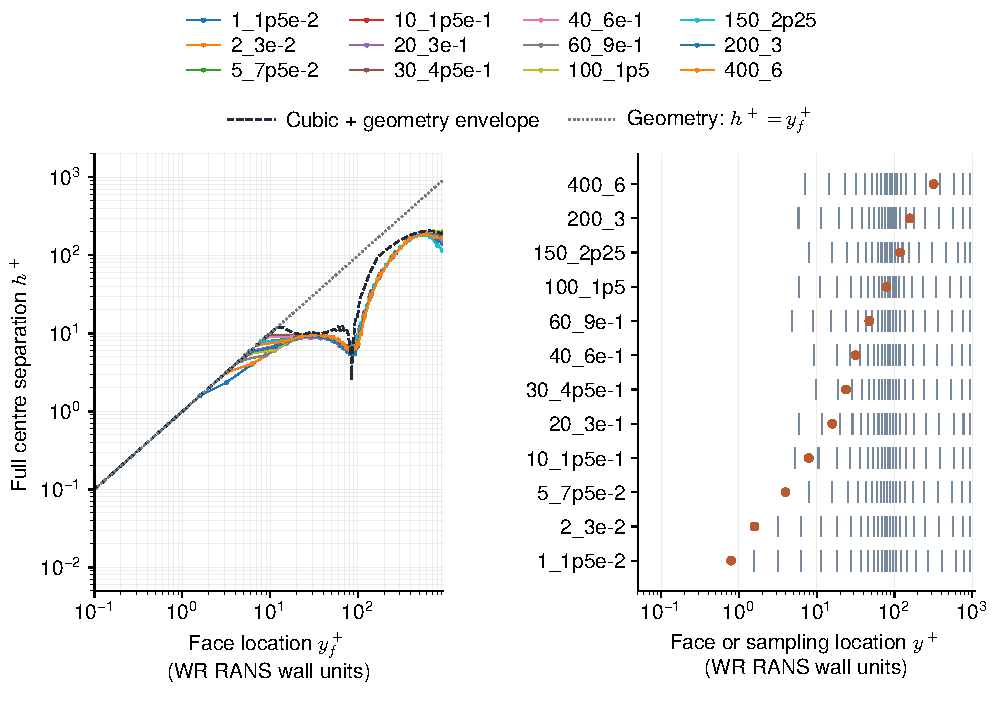
\includegraphics[width=\linewidth]{07_Error_Isolation_Results/Figures/WallFunctions/LowHM3_mesh_sweep_3pct.pdf}
    \caption{Boundary layer-informed $3\%$ spatial discretization error mesh family for LowH\_M3. The naming of the mesh families follows the structure \textit{desired wall-function sampling point in $y^+$}\_\textit{desired wall-function sampling point in millimetres}. Left: Black dotted and dashed lines represent the envelope stemming from the boundary layer analysis as described in Section~\ref{subsec:comparative:zpg:mesh-criterion}. The colourfull lines show the new boundary layer-informed meshes' actual spatial discretization error against the known boundary layer profiles, with all of them consistently staying below the $3\%$ envelope. Right: The actual mesh design (blue lines represent the position of the cell faces) and wall-function sampling centres (orange) are shown, with the pronounced clustering around the $y^+\approx85$ where the temperature peak sits for this case.} 
    \label{fig:WF:LowHM3-3pct-mesh-sweep}
\end{figure}

\begin{figure}[H]
    \centering
    % Figure provenance (WSL; absolute paths):
    %   Figure: /home/mgnadlinger/Xue_et_al/flat_plate/M6Tw025/opt_mesh/spacing_limits/M6Tw025_mesh_sweep_3pct.png
    %   Python script:
    %     /home/mgnadlinger/Xue_et_al/flat_plate/M6Tw025/opt_mesh/scripts/plot_analysis.py
    %   Data / simulation roots (high-level):
    %     /home/mgnadlinger/Xue_et_al/flat_plate/M6Tw025/opt_mesh/searches/3pct
    %     /home/mgnadlinger/Xue_et_al/flat_plate/M6Tw025/opt_mesh/Li_3pct_SA
    %     /home/mgnadlinger/Xue_et_al/flat_plate/M6Tw025/opt_mesh/spacing_limits
    %     /home/mgnadlinger/Xue_et_al/flat_plate/M6Tw025/opt_mesh/reference
    %     /home/mgnadlinger/Xue_et_al/flat_plate/M6Tw025/Digitizations
    %     /home/mgnadlinger/Xue_et_al/flat_plate/M6Tw025/Li_SA/SA_Prt0p9_baseline
    %   Note: Source report identifies this as the ordinary-Li mesh family.
    % End figure provenance.
    %   Print-size typography: regenerated at 170 mm width with 10 pt text; exact source data
    %     and local plotting script retained in Figures/WallFunctions/mesh_sweep_font_sources/.
    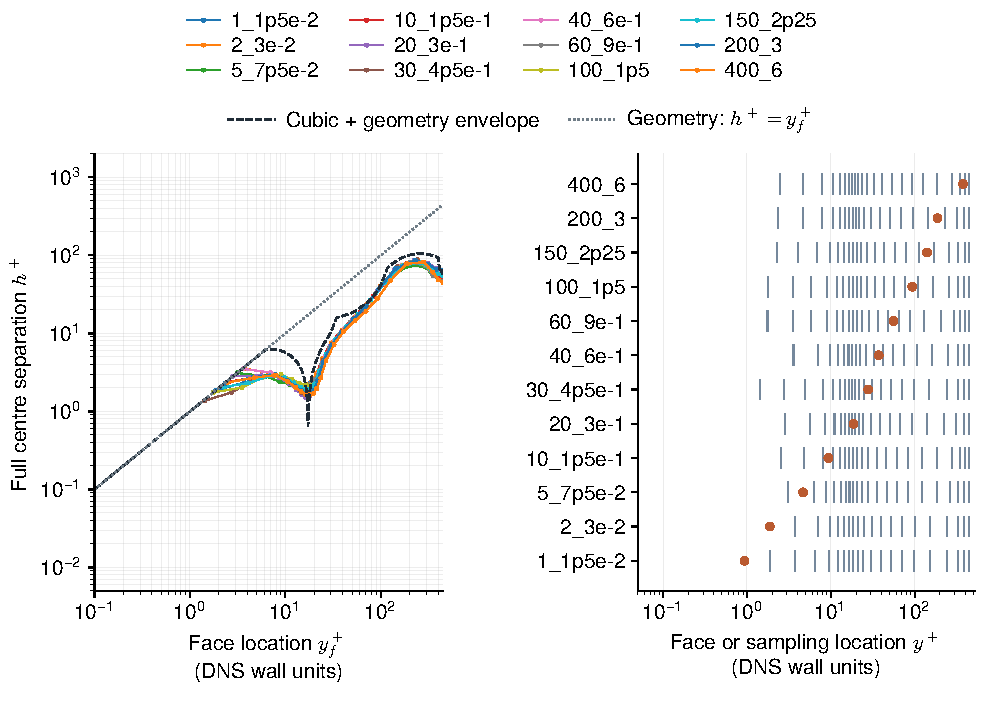
\includegraphics[width=\linewidth]{07_Error_Isolation_Results/Figures/WallFunctions/M6Tw025_mesh_sweep_3pct.pdf}
    \caption{Boundary layer-informed $3\%$ spatial discretization error mesh family for M6Tw025. The naming of the mesh families follows the structure \textit{desired wall-function sampling point in $y^+$}\_\textit{desired wall-function sampling point in millimetres}. Left: Black dotted and dashed lines represent the envelope stemming from the boundary layer analysis as described in Section~\ref{subsec:comparative:zpg:mesh-criterion}. The colourfull lines show the new boundary layer-informed meshes' actual spatial discretization error against the known boundary layer profiles, with all of them consistently staying below the $3\%$ envelope. Right: The actual mesh design (blue lines represent the position of the cell faces) and wall-function sampling centres (orange) are shown, with the pronounced clustering around the $y^+\approx18$ where the temperature peak sits for this case.}
    \label{fig:WF:M6Tw025-3pct-mesh-sweep}
\end{figure}

Figure~\ref{fig:WF:3pct-bl-informed-mesh-CFD-results} presents the CFD sweeps on these meshes. The abscissa is now the wall-function's sample location $y_s^+$, rather than necessarily the physical first-cell $y_1^+$. The reader is encouraged to look at the a-priori analysis, conventional coarase wall-function mesh CFD and herein presented boundary layer-informed mesh CFD results side by side for the four investigated combionations of Li wall function and Griffin wall function on the LowH\_M3 and M6Tw025 case (e.g. for the Li wall function on the LowH\_M3 case, see Figures~\ref{fig:wall-closure:a-priori-Li-LowHM3},~\ref{fig:WF:Li-LowHM3_conventional_mesh} and~\ref{fig:WF:3pct-bl-informed-mesh-CFD-results} top).
\par\medskip

It is immediatly apparant that the boundary layer-informed meshes follow the general error trend of the a-priori found closure error, significantly better than the conventional coarse wall-function meshes. The pronounced overshoot in the buffer layer that the conventional mesh exhibits in Figure~\ref{fig:WF:Li-LowHM3_conventional_mesh} is removed and the boundary layer-informed meshes in Figure~\ref{fig:WF:3pct-bl-informed-mesh-CFD-results} (top) show significantly closer trend to the a-priori results of Figure~\ref{fig:wall-closure:a-priori-Li-LowHM3}. Also indicative is, that Figure~\ref{fig:WF:Li-LowHM3_conventional_mesh} from $y^+\approx2$ onwards deviated from the wall-resolved baseline, whereas the boundary layer-informed meshes in Figure~\ref{fig:WF:3pct-bl-informed-mesh-CFD-results} (top) follow the a-priori in Figure~\ref{fig:wall-closure:a-priori-Li-LowHM3}, of effectly zero error, up to the same $y^+\approx10$.
\par\medskip

Because of error addition and cancellation, the wall-function CFD results on the boundary layer-informed meshes do not exactly match the quantiataive errors of the a-priori analysis. Arguably an even finer boundary layer-informed mesh with $\epsilon_max \le 0.1\%$ could be designed to further isolate the discretization errors, this highlights how big of an impact even these small discretization errors can have. For comparing the M6Tw025 cases, one should also keep in mind, that an additonal uncertainty arises in the discovered fact, that the turbulence model is not capable to reproduce the DNS temperature peak, as discussed in Section~\ref{subsec:comparative:zpg:wr-profiles} and investigated implications in Section~\ref{subsec:erriso:rans-profile-influence}.
\par\medskip

The highest sampling positions require particular caution. The LowH\_M3 Li curve rises markedly at its outermost sample, where inner-layer and approximately constant-stress assumptions become less suitable as discussed in the a-prori analysis in Section~\ref{subsec:comparative:zpg:apriori-mesh}. This point does not establish a general acceptable upper $y_s^+$, since the relevant boundary layer region and the closure's usable range are case dependent.
\par\medskip

From the analysis there is a strong conclusion from the CFD results of the herin used boundary layer-informed meshes vs. the previous conventional meshes, that the large error in the buffer layer and lower log-layer is driven by the spatial discretization error discussed as hypthesized.

\begin{figure}[H]
    \centering
    % Figure provenance (WSL; absolute paths):
    %   Figure: /home/mgnadlinger/WF_validation/LowH_M3/validation/outputs/plots/opt_mesh/li_3pct_mincells_sa_dns_station_relative_error.png
    %   Python scripts:
    %     /home/mgnadlinger/WF_validation/LowH_M3/validation/scripts/plot_opt_mesh_wall_flux_sweeps.py
    %     /home/mgnadlinger/WF_validation/LowH_M3/validation/scripts/plot_wall_flux_sweeps.py
    %   Data / simulation roots (high-level):
    %     /home/mgnadlinger/WF_validation/LowH_M3/opt_meshes/Li_3pct_minCells_SA
    %     /home/mgnadlinger/WF_validation/LowH_M3/wall_resolved/SA/LowH_M3
    %     /home/mgnadlinger/WF_validation/LowH_M3/Digitizations
    %   Note: Thesis image removes the 128-pixel title strip from the source export.
    % End figure provenance.
    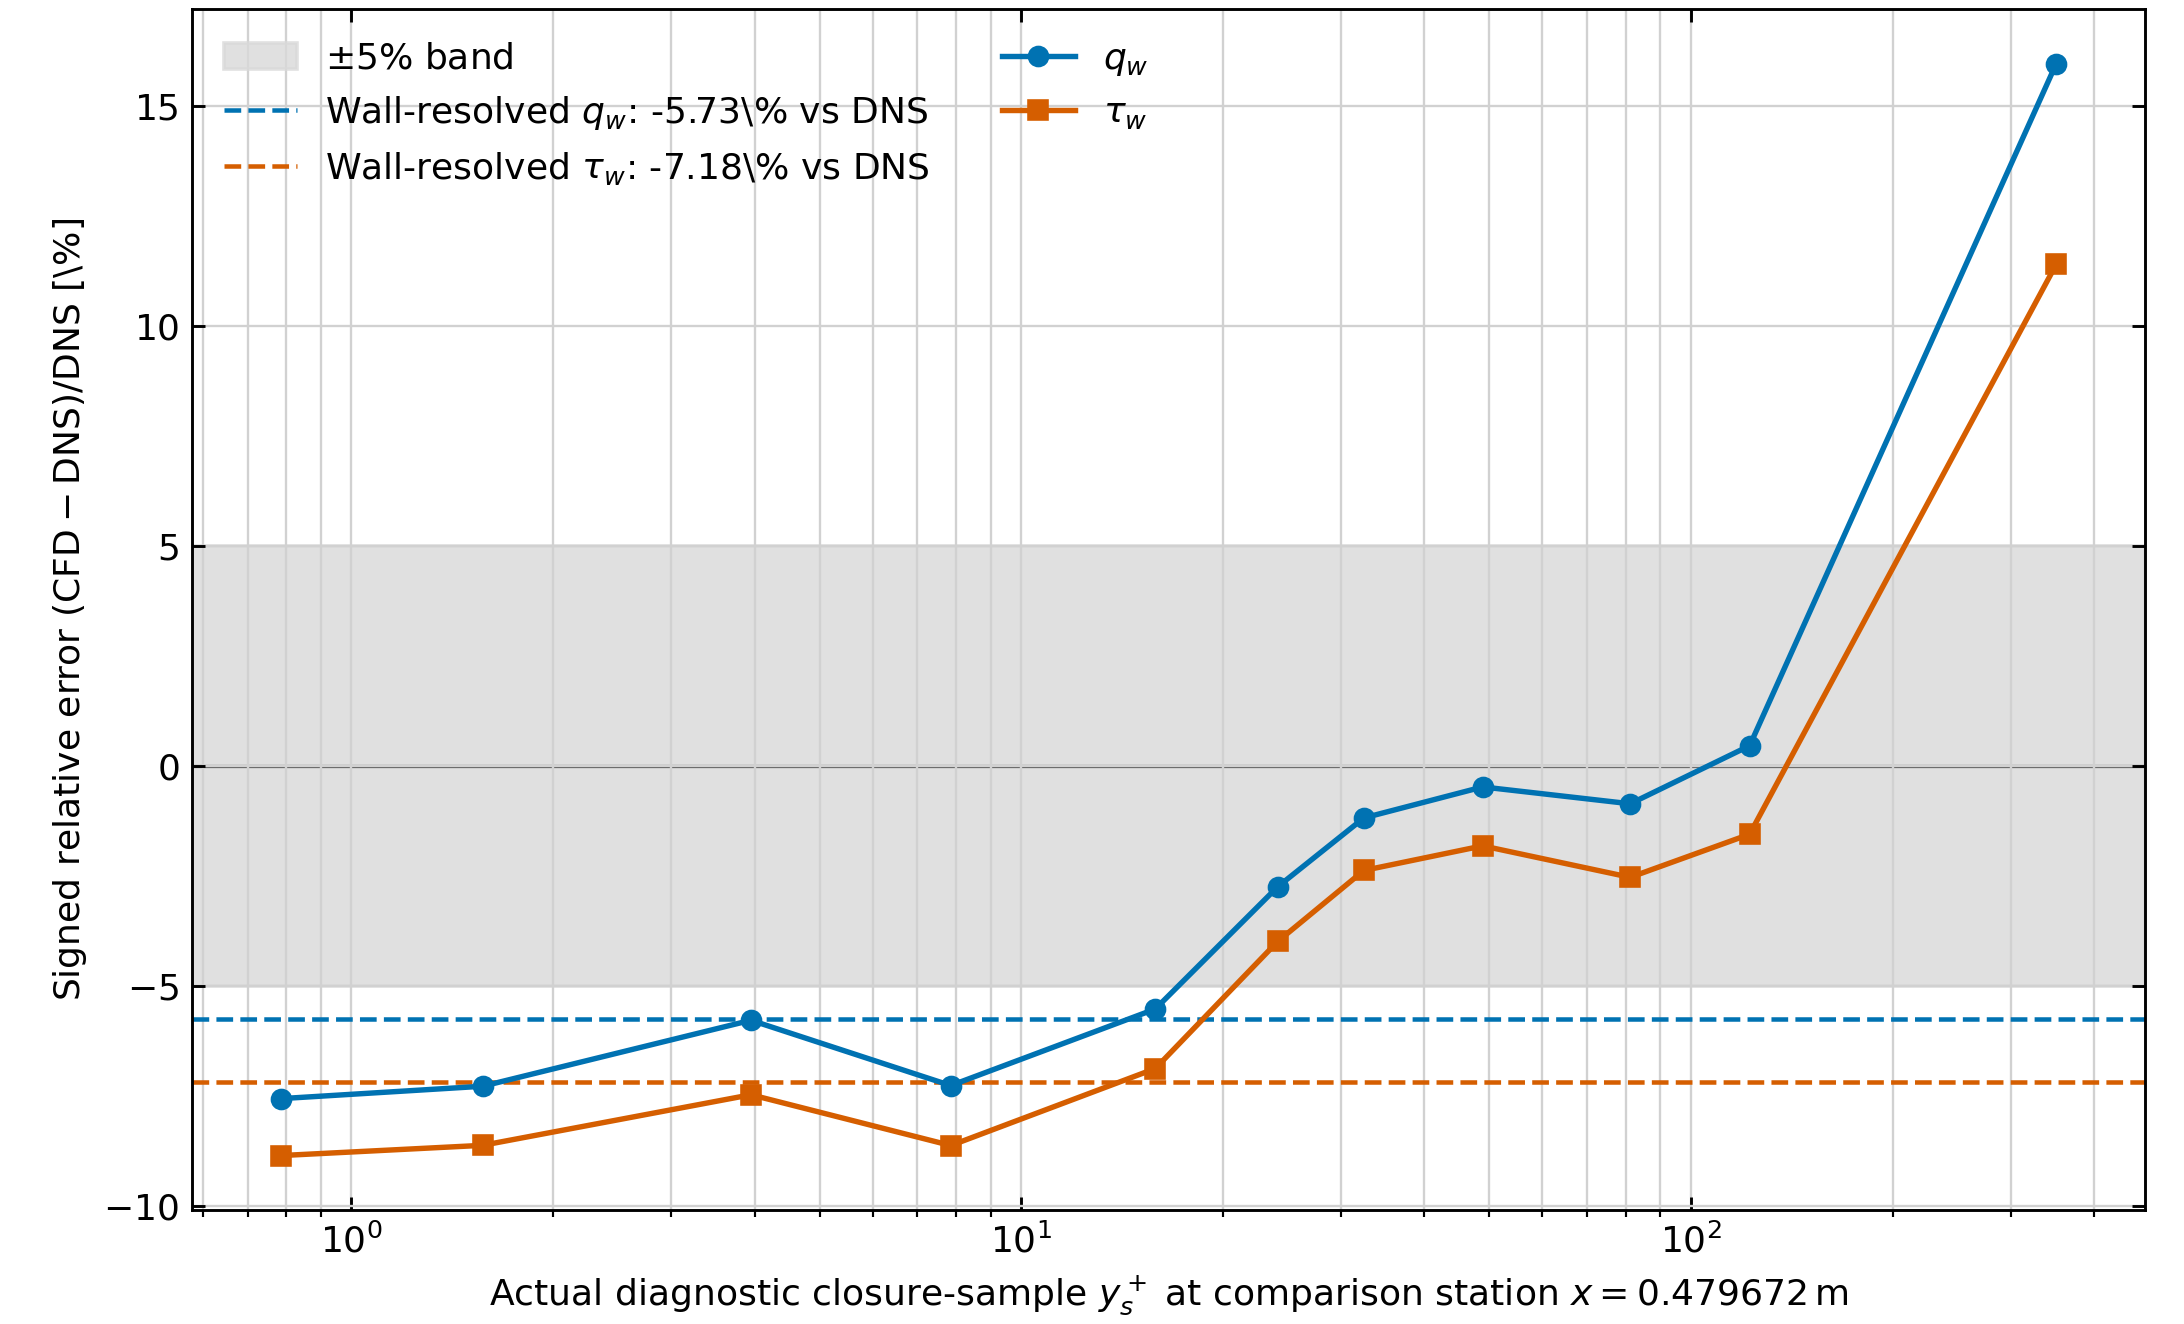
\includegraphics[width=\linewidth,height=.40\textheight,keepaspectratio]{07_Error_Isolation_Results/Figures/WallFunctions/04_3pctMesh_Li_LowHM3.png}
    % Figure provenance (WSL; absolute paths):
    %   Figure: /home/mgnadlinger/WF_validation/LowH_M3/validation/outputs/plots/opt_mesh/griffin_3pct_mincells_sa_dns_station_relative_error.png
    %   Python scripts:
    %     /home/mgnadlinger/WF_validation/LowH_M3/validation/scripts/plot_opt_mesh_wall_flux_sweeps.py
    %     /home/mgnadlinger/WF_validation/LowH_M3/validation/scripts/plot_wall_flux_sweeps.py
    %   Data / simulation roots (high-level):
    %     /home/mgnadlinger/WF_validation/LowH_M3/opt_meshes/Griffin_3pct_minCells_SA
    %     /home/mgnadlinger/WF_validation/LowH_M3/wall_resolved/SA/LowH_M3
    %     /home/mgnadlinger/WF_validation/LowH_M3/Digitizations
    % End figure provenance.
    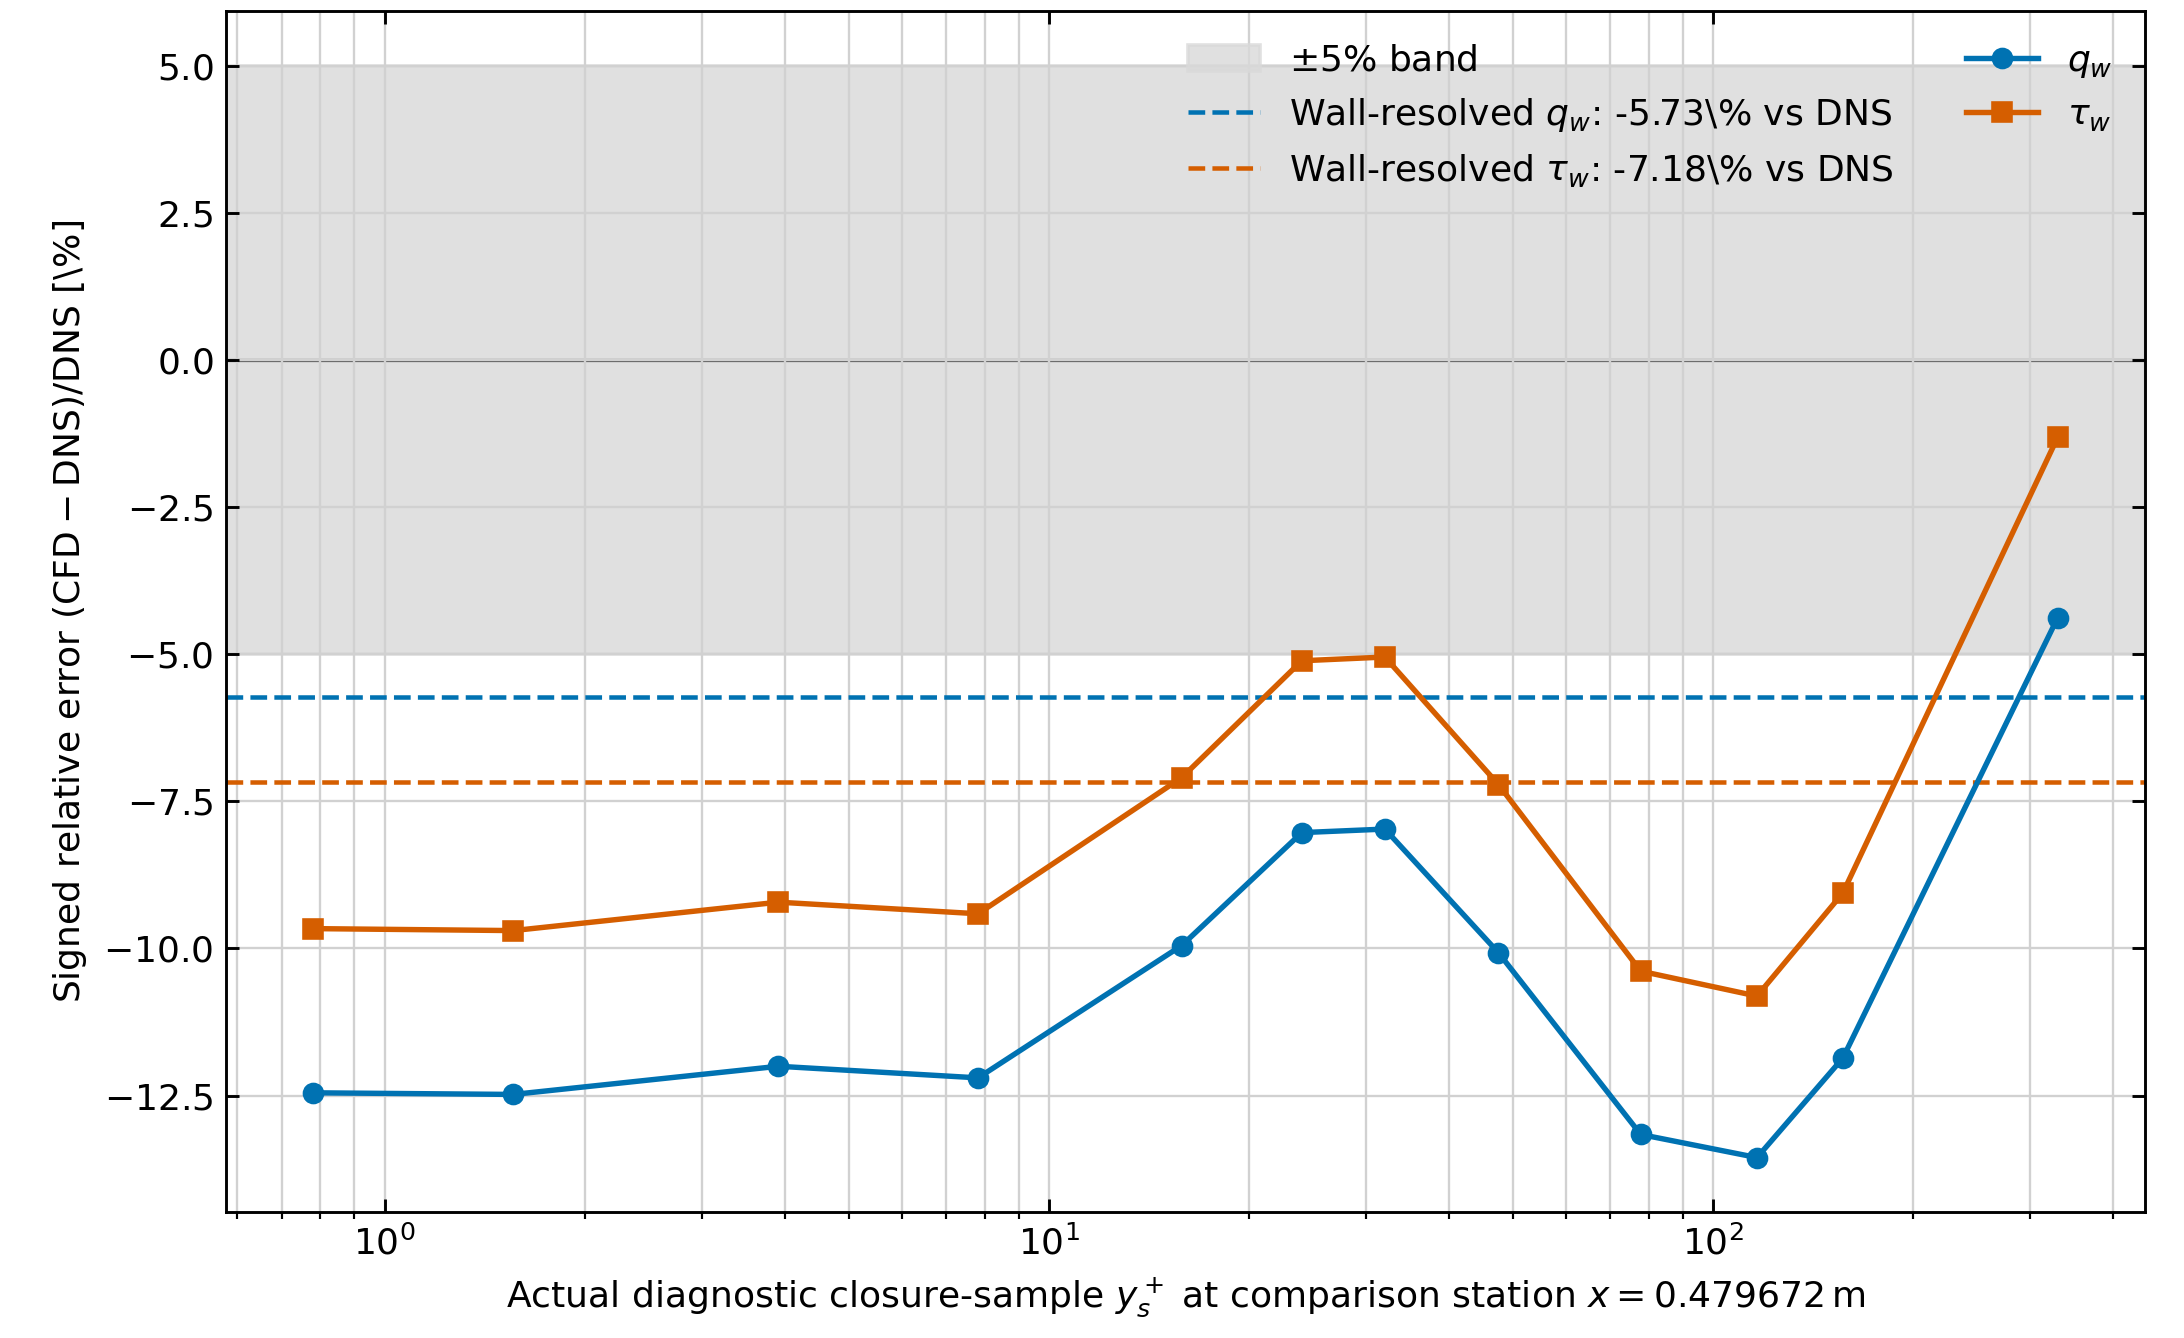
\includegraphics[width=\linewidth,height=.40\textheight,keepaspectratio]{07_Error_Isolation_Results/Figures/WallFunctions/04_3pctMesh_Griffin_LowHM3.png}
    \caption{Wall-function CFD on boundary layer-informed meshes designed with the $3\%$ cubic-reference component criterion. LowH\_M3 results are shown for Li (top) and Griffin (bottom). The abscissa is the actual diagnostic sampling location $y_s^+$ for the wall-function, not the first cell height. Dashed lines denote the wall-resolved baseline; shading marks $\pm5\%$ relative to DNS.}
    \label{fig:WF:3pct-bl-informed-mesh-CFD-results}
\end{figure}q

\begin{figure}[H]
    \ContinuedFloat
    \centering
    % Figure provenance (WSL; absolute paths):
    %   Figure: /home/mgnadlinger/Xue_et_al/flat_plate/M6Tw025/validation/outputs/plots/opt_mesh/li_3pct_sa_dns_station_relative_error.png
    %   Python scripts:
    %     /home/mgnadlinger/Xue_et_al/flat_plate/M6Tw025/validation/scripts/plot_opt_mesh_wall_flux_sweeps.py
    %     /home/mgnadlinger/Xue_et_al/flat_plate/M6Tw025/validation/scripts/plot_wall_flux_sweeps.py
    %   Data / simulation roots (high-level):
    %     /home/mgnadlinger/Xue_et_al/flat_plate/M6Tw025/opt_mesh/Li_3pct_SA
    %     /home/mgnadlinger/Xue_et_al/flat_plate/M6Tw025/Li_SA/SA_Prt0p9_baseline
    %     /home/mgnadlinger/Xue_et_al/flat_plate/M6Tw025/Digitizations
    %     /home/mgnadlinger/Xue_et_al/flat_plate/M6Tw025/opt_mesh/reference/sources
    % End figure provenance.
    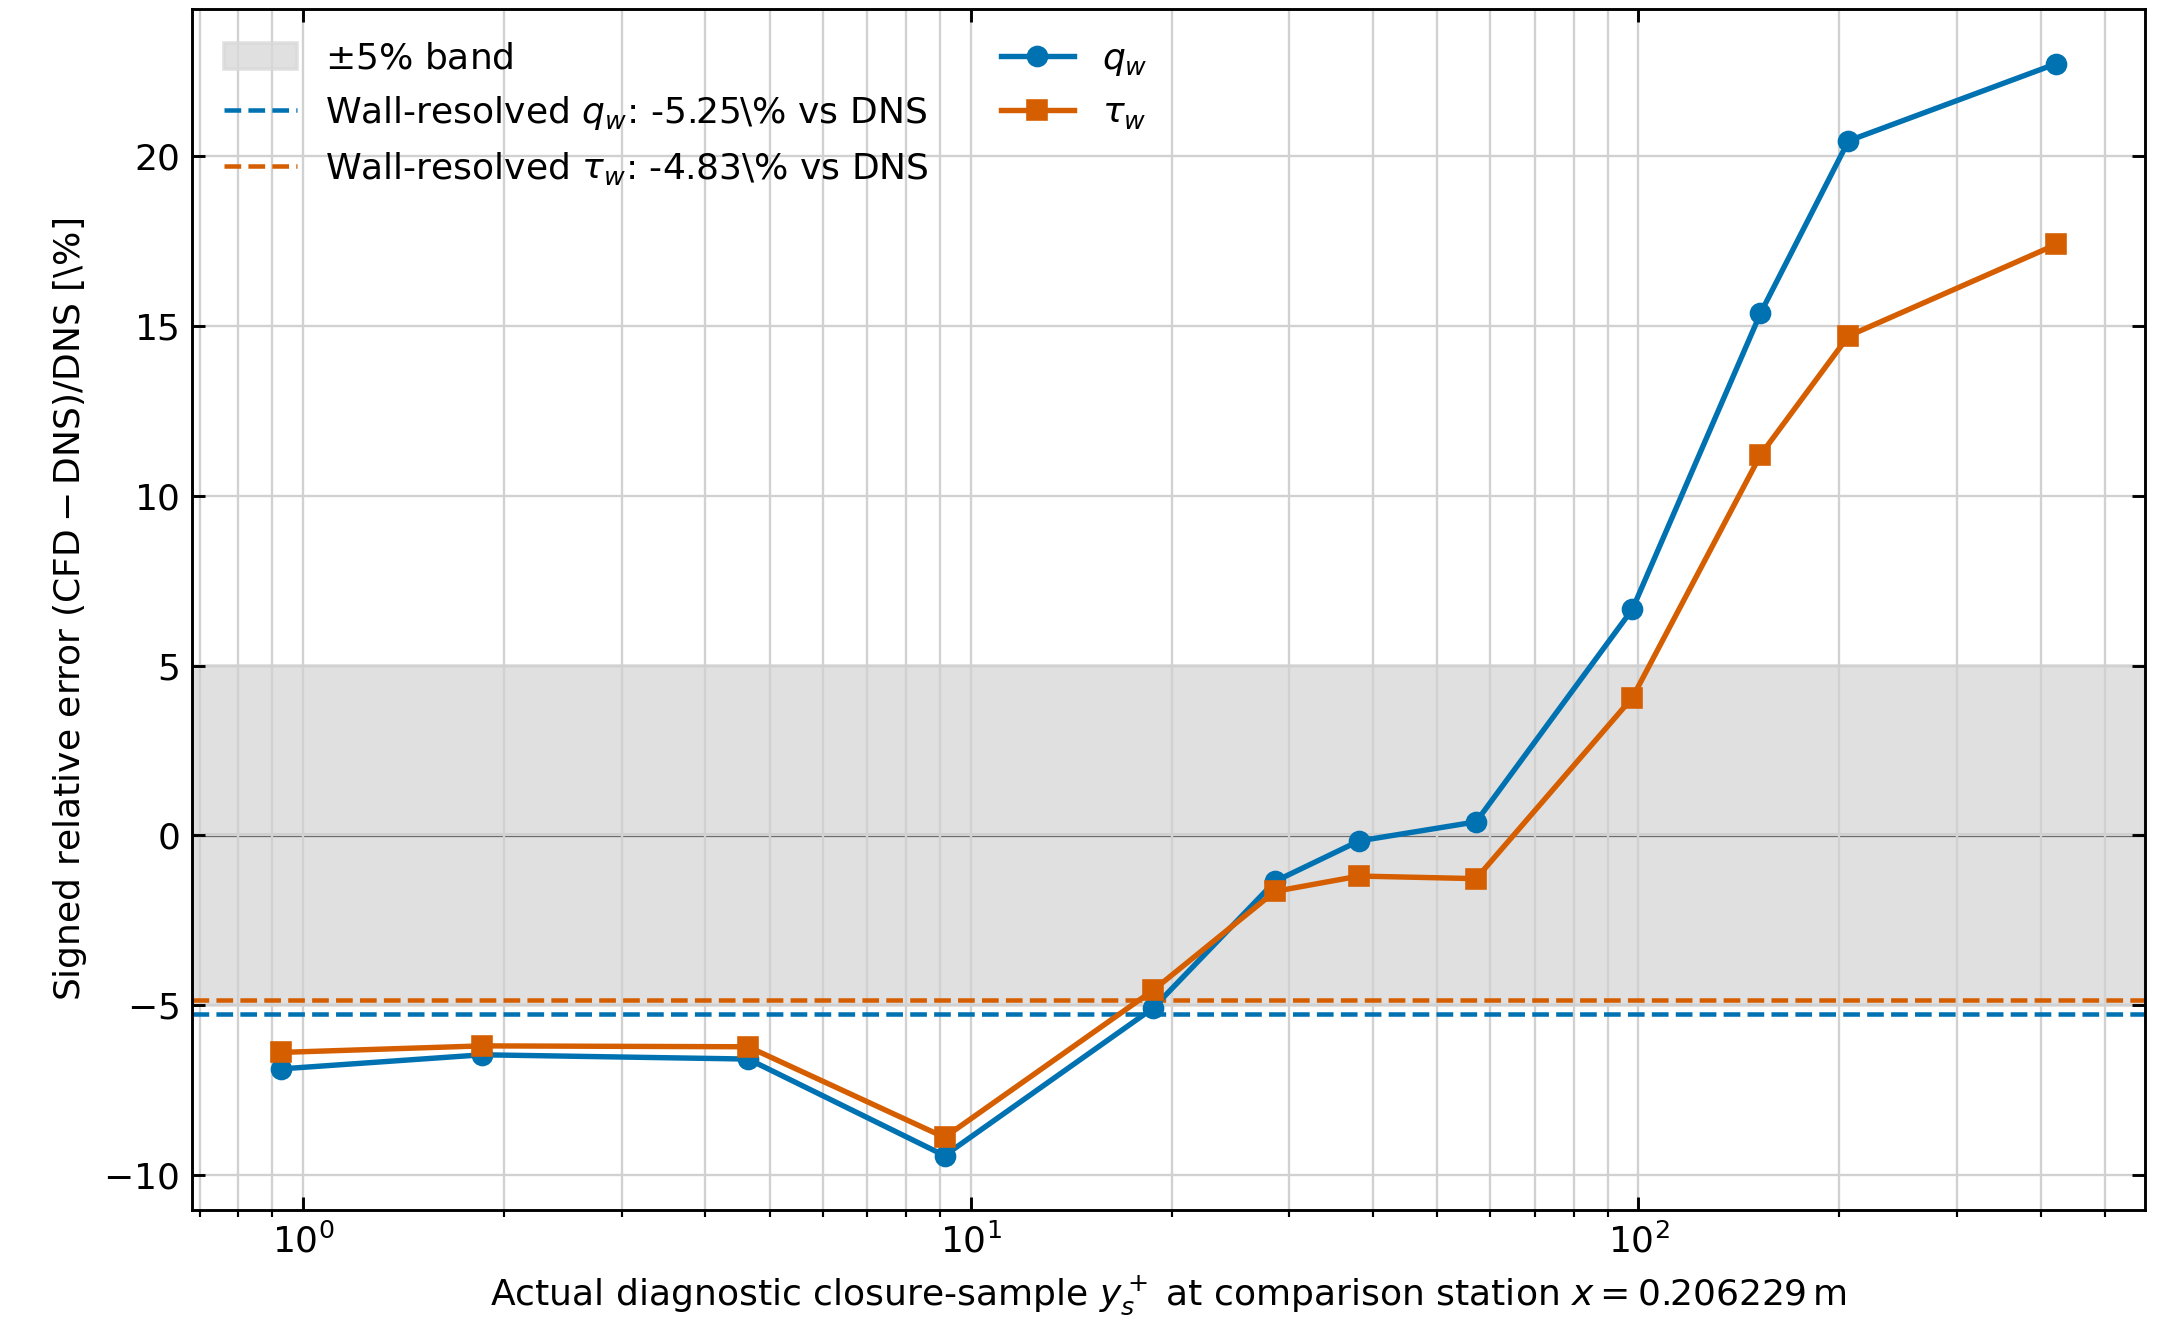
\includegraphics[width=\linewidth,height=.40\textheight,keepaspectratio]{07_Error_Isolation_Results/Figures/WallFunctions/04_3pctMesh_Li_M6Tw025.png}
    % Figure provenance (WSL; absolute paths):
    %   Figure: /home/mgnadlinger/Xue_et_al/flat_plate/M6Tw025/validation/outputs/plots/opt_mesh/griffin_3pct_sa_dns_station_relative_error.png
    %   Python scripts:
    %     /home/mgnadlinger/Xue_et_al/flat_plate/M6Tw025/validation/scripts/plot_opt_mesh_wall_flux_sweeps.py
    %     /home/mgnadlinger/Xue_et_al/flat_plate/M6Tw025/validation/scripts/plot_wall_flux_sweeps.py
    %   Data / simulation roots (high-level):
    %     /home/mgnadlinger/Xue_et_al/flat_plate/M6Tw025/opt_mesh/Griffin_3pct_SA
    %     /home/mgnadlinger/Xue_et_al/flat_plate/M6Tw025/Li_SA/SA_Prt0p9_baseline
    %     /home/mgnadlinger/Xue_et_al/flat_plate/M6Tw025/Digitizations
    %     /home/mgnadlinger/Xue_et_al/flat_plate/M6Tw025/opt_mesh/reference/sources
    % End figure provenance.
    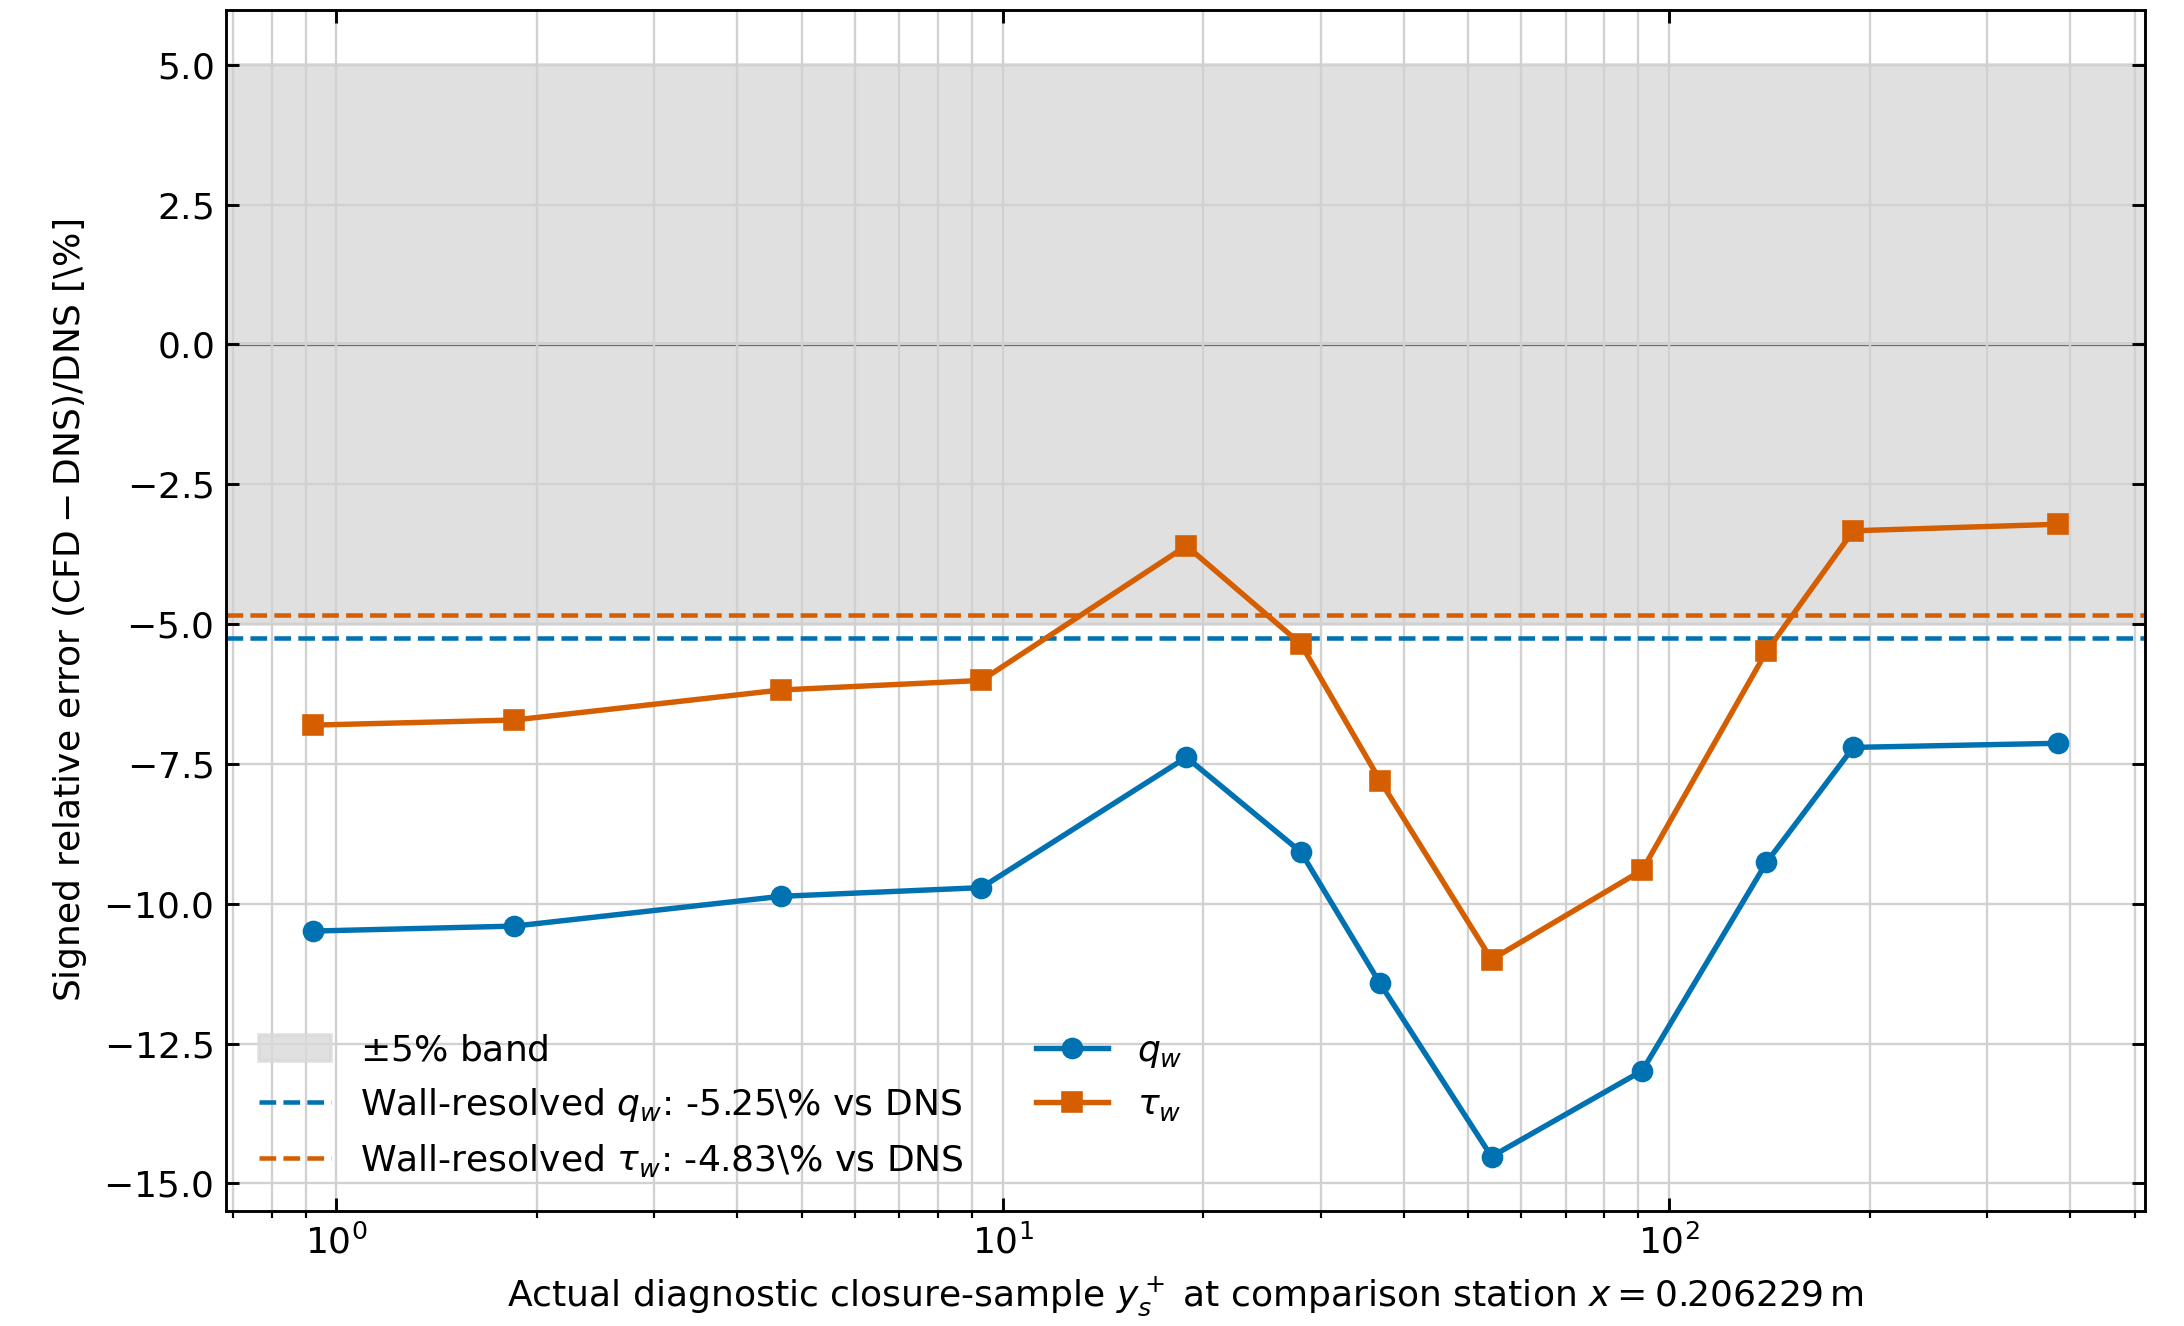
\includegraphics[width=\linewidth,height=.40\textheight,keepaspectratio]{07_Error_Isolation_Results/Figures/WallFunctions/04_3pctMesh_Griffin_M6Tw025.png}
    \caption[]{M6Tw025 results for Li (top) and Griffin (bottom), with SA and DNS normalization at $x=0.206229\,\mathrm{m}$. The mesh criterion and sampling-height definition are the same as in the preceding panels.}
\end{figure}

\subsection{Conditional a-priori estimation of the mesh requirement}
\label{subsec:comparative:zpg:apriori-mesh}

The above analysis and the novel proposed boundary layer informed meshing criterion, has one practical shortcoming: it requires knowledge of the resolved boundary layer profile. For an engineering approach, it is desirable to have a mesh design tool that does not require the resolved profile, but can still provide a-priori guidance on the required mesh spacing. The closures of the analytical Li et al. wall-function \cite{li2025WF} have this knowledge about hypersonic boundary layer backed in by design. Given wall shear and heat-flux, wall thermodynamic and transport properties, and an edge state, the wall-function closures can reconstruct the underlying profiles from which then the same finite-stencil limits can be evaluated. In the constant-$c_p$ form used here, the enthalpy relation supplies temperature from velocity, and the velocity law supplies the wall-normal coordinate. Under the additional constant-total-shear assumption, effective viscosity follows from $\mu_{\mathrm{eff}}=\tau_w/(\partial U/\partial y)$. Prescribed molecular and turbulent Prandtl numbers then give an effective conductivity estimate.
\par\medskip

Figure~\ref{fig:WF:a-priori-M6Tw025-10pct-envelope-combined} compares this estimate with the M6Tw025 profile-based envelope at a $10\%$ error tolerance. The reconstruction uses scalar DNS metadata for the wall loads and edge/wall states, without using the resolved profile values. It is therefore an assessment conditional on known loads, rather than an independent prediction of those loads. The broad inner-layer spacing trend is recovered, but the most restrictive minimum is shifted because the Li reconstruction places the temperature maximum closer to the wall. Near that maximum, even a modest position error can produce a large difference in the relative-gradient criterion. Differences toward the boundary layer edge also reflect the limited outer-layer representation of the reconstructed inner law.

\begin{figure}[H]
    \centering
    % Figure provenance (WSL; absolute paths):
    %   Figure: /home/mgnadlinger/Xue_et_al/flat_plate/M6Tw025/opt_mesh/li_apriori/M6Tw025_Li_combined_comparison_10pct_only.png
    %   Python scripts:
    %     /home/mgnadlinger/Xue_et_al/flat_plate/M6Tw025/opt_mesh/li_apriori/plot_10pct_combined_only.py
    %     /home/mgnadlinger/Xue_et_al/flat_plate/M6Tw025/opt_mesh/li_apriori/li_apriori_spacing.py
    %   Data / simulation roots (high-level):
    %     /home/mgnadlinger/Xue_et_al/flat_plate/M6Tw025/opt_mesh/li_apriori
    %     /home/mgnadlinger/Xue_et_al/flat_plate/M6Tw025/opt_mesh/spacing_limits
    %     /home/mgnadlinger/Xue_et_al/flat_plate/M6Tw025/opt_mesh/reference
    %     /home/mgnadlinger/Xue_et_al/flat_plate/M6Tw025/Digitizations
    %     /home/mgnadlinger/Xue_et_al/flat_plate/M6Tw025/Li_SA/SA_Prt0p9_baseline
    %   Note: Thesis image is cropped from the source export at native resolution, without resizing.
    %     Crop box in source pixels (left, top, right, bottom): (0, 274, 2250, 2200);
    %     resulting size: 2250 x 1926 pixels. Original plot proportions are preserved.
    %   Note: li_apriori_spacing.py generates the prediction from DNS scalar header inputs; the frozen DNS/SA
    %     reference supplies the comparison envelope.
    % End figure provenance.
    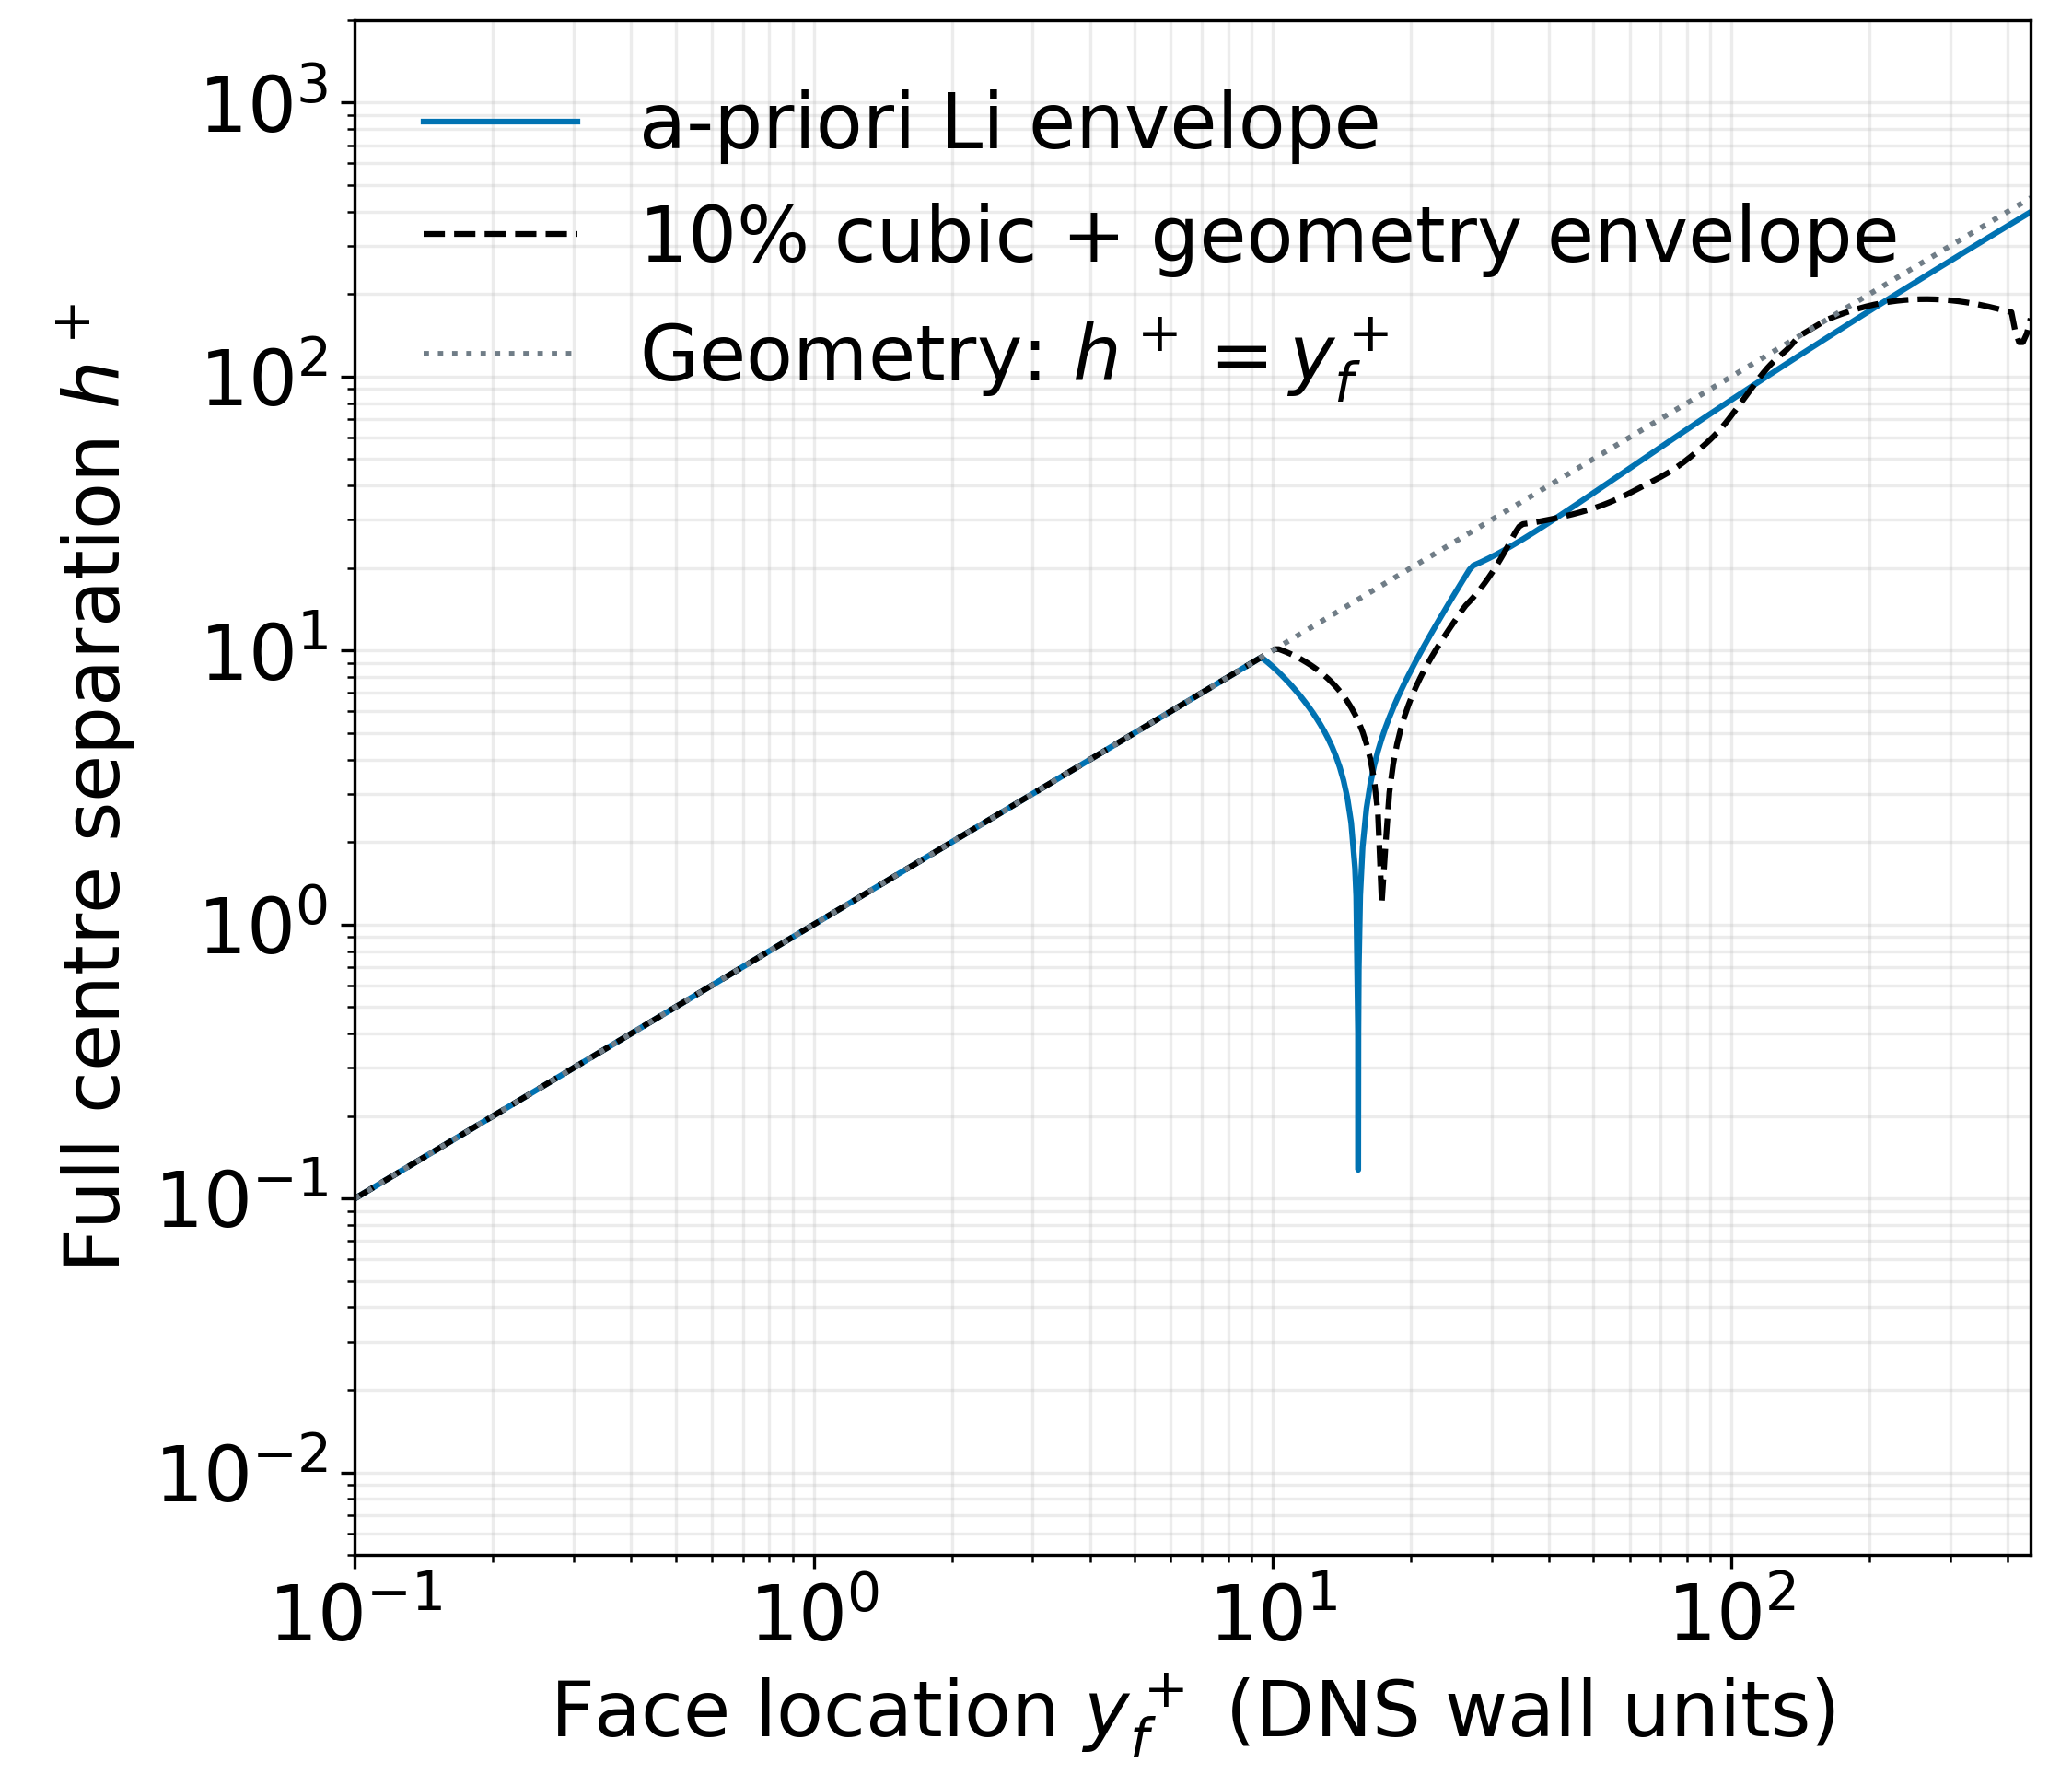
\includegraphics[width=.7\linewidth,height=.54\textheight,keepaspectratio]{07_Error_Isolation_Results/Figures/WallFunctions/apriori_M6_mesh.png}
    \caption{Conditional a-priori estimate of the M6Tw025 $10\%$ spacing envelope from the Li relations (blue), compared with the profile-based cubic-reference envelope (black dashed). The reconstruction uses scalar wall loads, wall/edge states and transport properties, without the resolved boundary layer profile. The geometric cap is dotted. The displaced restrictive minimum near the temperature maximum limits the estimate's use as an accuracy guarantee.}
    \label{fig:WF:a-priori-M6Tw025-10pct-envelope-combined}
\end{figure}

The estimate can consequently guide an initial mesh design or identify a likely region of refinement. Practical use also requires suitable estimates of wall loads and edge quantities. For the present zero-pressure-gradient flat-plates these inputs are comparatively well defined. The boundary layer edge states can be approximated to the freestream conditions, and for the wall heat-flux and shear stress on zero-pressure-gradient flat-plates analytical approximations like the theory of van Driest are available. Their approximation and the validity of the equilibrium assumptions are however more challenging for complex flows.

\subsection{Recovery of the wall-resolved baseline with fitted closures}
\label{subsec:comparative:zpg:fitted-closure}
 
The remaining question, to close the error isolation loop, is whether the wall-function formulation can recover the wall-resolved solution when both its closure relations and spatial discretization errors are removed. LowH\_M3 provides a suitable diagnostic case because its wall-resolved SA thermal-profile shape agrees comparatively well with DNS, thus also eliviating the implications of the turbulence model. The Li formulation is retained, but its velocity and enthalpy relations are fitted to the wall-resolved SA field of the LowH\_M3 case.
\par\medskip

Lookup tables for the wall function's momentum and enthalpy closures are constructed from the wall-resolved SA boundary layer profiles, using the reference wall shear stress, wall heat-flux and local boundary layer edge velocity and temperature. The tables store the fitted velocity relation and a correction to the Li enthalpy relation. During CFD, the fitted closure relations determine wall shear stress and wall heat-flux from the wall-function sample station's velocity and temperature, while the fitted velocity-law derivative supplies the near-wall constraint on the SA variable $\tilde{\nu}$ (Section~\ref{subsec:wall-functions:gao-li:turbulence-coupling}). The construction therefore requires reference profiles at multiple streamwise stations and the singular published DNS profiles are insufficient.
\par\medskip

Figure~\ref{fig:WF:a-priori-Li-fitted-LowHM3} first checks the fitted closure relations using the same a-priori approach as in Section~\ref{subsec:erriso:apriori-solver}. The recovered heat-flux and shear stress differ from the wall-resolved targets by order $10^{-7}\%$. This near-exact recovery verifies the reference-conditioned inverse construction at the sampled states.

\begin{figure}[H]
    \centering
    % Figure provenance (WSL; absolute paths):
    %   Figure: /home/mgnadlinger/OpenFOAM/mgnadlinger-v2412/src/LiWallFunctions/tests/ReverseSolver/LowH_M3_Duan_Li_fitted/wall_flux_errors_vs_yplus.png
    %   Python scripts:
    %     /home/mgnadlinger/OpenFOAM/mgnadlinger-v2412/src/LiWallFunctions/tests/ReverseSolver/analyze_li_fitted_wall_function_profile_Duan.py
    %     /home/mgnadlinger/OpenFOAM/mgnadlinger-v2412/src/LiWallFunctions/tests/ReverseSolver/build_lowh_m3_fitted_model.py
    %   Data / simulation roots (high-level):
    %     /home/mgnadlinger/OpenFOAM/mgnadlinger-v2412/src/LiWallFunctions/tests/ReverseSolver/LowH_M3_Duan
    %     /home/mgnadlinger/OpenFOAM/mgnadlinger-v2412/src/LiWallFunctions/tests/ReverseSolver/LowH_M3_Duan_Li/constant/LiLowHM3Fit
    %     /home/mgnadlinger/OpenFOAM/mgnadlinger-v2412/src/LiWallFunctions/tests/ReverseSolver/LowH_M3_Duan_Li_fitted
    %     /home/mgnadlinger/Duan_DNS_ZPGFP/Martin_Duan_Part4/SA_Prt0p9/LowH_M3
    %     /home/mgnadlinger/WF_validation/LowH_M3/wall_resolved/SA/LowH_M3
    %     /home/mgnadlinger/WF_validation/LowH_M3/Li_SA
    %   Note: Closure input is the wall-resolved SA profile at time 20000.
    %   Note: Thesis image is resized from the source export. The fitted model uses wall-resolved SA profiles
    %     and Li_SA mesh geometry.
    % End figure provenance.
    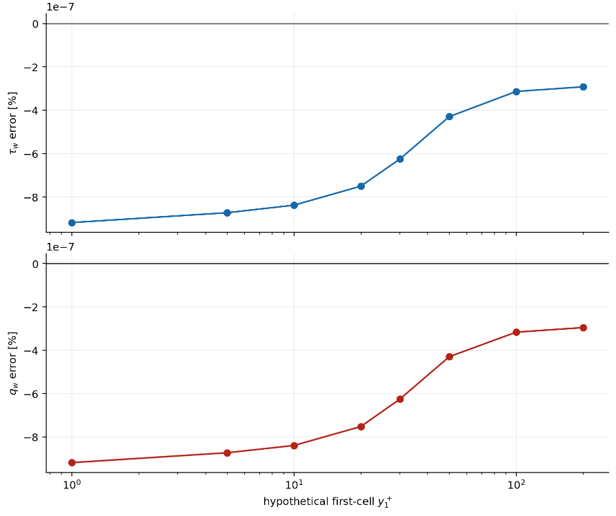
\includegraphics[width=\linewidth,height=.43\textheight,keepaspectratio]{07_Error_Isolation_Results/Figures/WallFunctions/a-priori-Li-fitted-LowHM3.png}
    \caption{A-priori inverse recovery using the fitted LowH\_M3 Li relations and samples from the wall-resolved SA reference. Recovered shear stress (top) and heat-flux (bottom) are compared with that same reference. Errors are of order $10^{-7}\%$, as indicated by the axis multipliers; this is consistency of the reference-conditioned inverse model, rather than independent DNS validation.}
    \label{fig:WF:a-priori-Li-fitted-LowHM3}
\end{figure}

The corresponding CFD result is shown in Figure~\ref{fig:WF:3pct-Li-fitted-LowHM3}. With the fitted relations and boundary layer-informed meshes, heat-flux and shear stress remain within approximately $\pm2\%$ of the wall-resolved values over the completed sampling sweep. Thus successfully isolating the errors caused by spatial discretization and wall-function closure theories. The last persistent error to the DNS reference, is the baseline error of the underlying wall-resolved RANS as discovered in the first Section~\ref{subsec:comparative:zpg:wr-wall-fluxes}. So it can be concluded, that with a boundary layer-informed mesh, improved closure relations and improved RANS turbulence modelling, the wall-function CFD could recover perfect wall heat-flux and shear stress.

\begin{figure}[H]
    \centering
    % Figure provenance (WSL; absolute paths):
    %   Figure: /home/mgnadlinger/WF_validation/LowH_M3/mesh_archives/20260908_before_leading_edge_refinement/Li_fitted_3pct_minCells_SA/results_analysis/wall_flux_sweep/plots/li_fitted_3pct_mincells_sa_dns_station_relative_error.png
    %   Python scripts:
    %     /home/mgnadlinger/WF_validation/LowH_M3/mesh_archives/20260908_before_leading_edge_refinement/Li_fitted_3pct_minCells_SA/results_analysis/run_wall_flux_sweep.py
    %     /home/mgnadlinger/WF_validation/LowH_M3/validation/scripts/plot_wall_flux_sweeps.py
    %   Data / simulation roots (high-level):
    %     /home/mgnadlinger/WF_validation/LowH_M3/mesh_archives/20260908_before_leading_edge_refinement/Li_fitted_3pct_minCells_SA
    %     /home/mgnadlinger/WF_validation/LowH_M3/wall_resolved/SA/LowH_M3
    %     /home/mgnadlinger/WF_validation/LowH_M3/Digitizations
    %   Note: Thesis image removes the 128-pixel title strip from the source export.
    %   Note: Displayed CFD results use the archived sweep from before the leading-edge mesh refinement on
    %     2026-09-08.
    %   Note: An identical full export is also retained at
    %     /home/mgnadlinger/WF_validation/LowH_M3/validation/outputs/plots/li_fitted_3pct_mincells_sa_dns_station_relative_error.png
    % End figure provenance.
    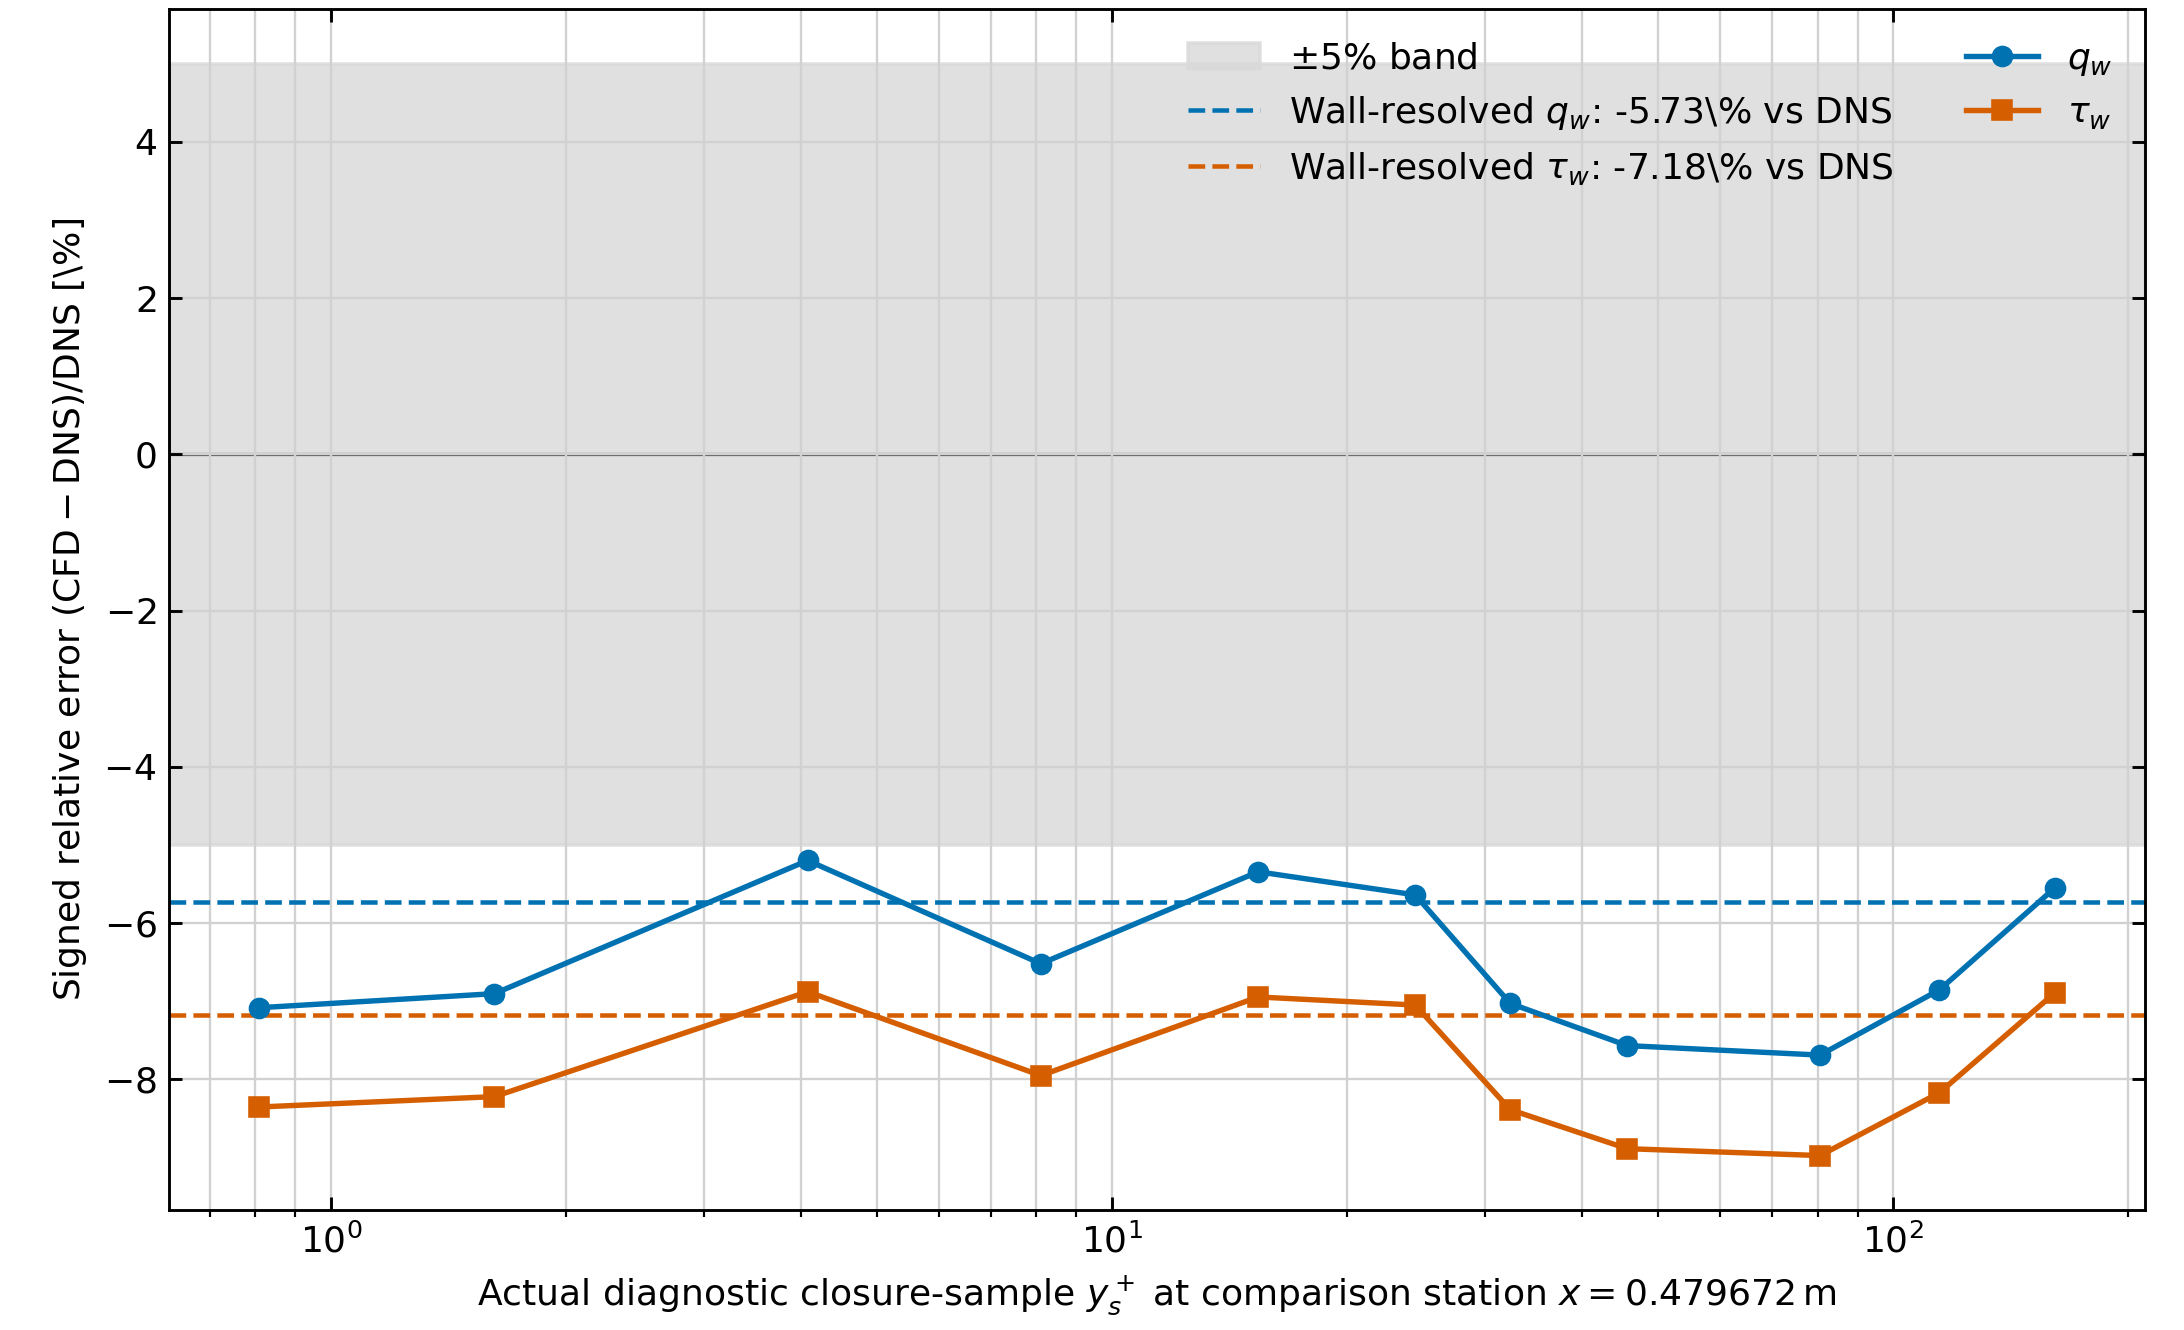
\includegraphics[width=\linewidth,height=.43\textheight,keepaspectratio]{07_Error_Isolation_Results/Figures/WallFunctions/04_3pctMesh_fitted_Li_LowHM3.png}
    \caption{LowH\_M3 CFD with fitted Li relations, SA and boundary layer-informed $3\%$ meshes. Signed errors in heat-flux and shear stress relative to DNS are plotted against the actual sampling location at $x=0.479672\,\mathrm{m}$. The curves remain close to the wall-resolved baseline (dashed), with deviations of approximately $\pm2\%$ when normalized by the corresponding wall-resolved quantities. Shading marks $\pm5\%$ relative to DNS.}
    \label{fig:WF:3pct-Li-fitted-LowHM3}
\end{figure}

